%%%%%%   TIPO DE DOCUMENTO: Artículo   %%%%%%
\documentclass[letterpaper,11pt,spanish]{report}

% ========================================
% CONFIGURACIÓN BÁSICA DEL DOCUMENTO
% ========================================
\usepackage[utf8]{inputenc}        % Soporte para caracteres especiales y acentos
\usepackage[spanish]{babel}        % Idioma español (traducciones y reglas tipográficas)
\usepackage{xspace}                 % Manejo inteligente de espacios después de comandos
\renewcommand{\baselinestretch}{1} % Interlineado simple

% --------------------------
% CONFIGURACIÓN DE TÍTULOS 
% --------------------------

%\titleformat{comando}{forma}
%   {formato}
%   {etiqueta}
%   {separacion}
%   {antes del titulo}
%   [despues del titulo]

\usepackage{titlesec}
\usepackage{etoolbox}

\titleformat{\chapter}[display] 
{\Large\raggedleft} 
{}
{0pt}
{
    \ifnum\value{chapter}>0 
        \rule{\textwidth}{0.5pt}
        \vspace{1ex}
        {\Large\bfseries\chaptername\ \thechapter \\}
        \vspace{1ex}
    \fi
} 
[
    \rule{\textwidth}{0.3pt}
] 


\titleformat{\section}
{\normalfont\bfseries\Large\raggedright}
{\thesection}
{1em}
{}

\titleformat{\subsection}
{\normalfont\bfseries\large\raggedright}
{\thesubsection}
{1em}
{}

% --------------------------
% CONFIGURACIÓN DE ENCABEZADOS CON FANCYHDR
% --------------------------
\usepackage{fancyhdr}

\renewcommand{\chaptermark}[1]{\markboth{#1}{}}
\fancypagestyle{mainstyle}{%
  \fancyhf{}
  \fancyhead[L]{\leftmark}
  \fancyhead[R]{\thepage}
  \fancyfoot{}
}

% --------------------------
% CONFIGURACIÓN DE ANEXOS
% --------------------------
\newcommand{\appendixtitleformat}{
  \titleformat{\chapter}[display]
    {\Large\raggedleft}
    {\appendixname\ \thechapter}
    {1ex}
    {\Large\bfseries}
    [\vspace{1ex}\rule{\textwidth}{0.3pt}]
}


% ========================================
% MATEMÁTICAS Y SÍMBOLOS
% ========================================
\usepackage{amsmath}                % Entornos matemáticos avanzados
\usepackage{amssymb}                % Símbolos matemáticos extendidos
\usepackage{amscd}                  % Diagramas conmutativos
\usepackage{amsthm}                 % Teoremas y entornos de demostración

% ========================================
% ALGORITMOS Y PSEUDOCÓDIGO
% ========================================
\usepackage{algorithm}              % Entornos para algoritmos
\usepackage{algpseudocode}          % Estilo para pseudocódigo

% ========================================
% GRÁFICOS E IMÁGENES
% ========================================
\usepackage{graphicx}               % Inclusión y manipulación de imágenes
\usepackage{subcaption}             % Subtítulos para subfiguras (subfigure)
\usepackage{tikz}                   % Creación de gráficos vectoriales
\usetikzlibrary{shapes, arrows}     % Formas y flechas para TikZ
\usetikzlibrary{arrows.meta}        % Estilos avanzados de flechas
\usetikzlibrary{positioning}        % Posicionamiento preciso de nodos

% ========================================
% CÓDIGO FUENTE Y LISTADOS
% ========================================
\usepackage{listings}               % Inclusión de código fuente
\renewcommand{\lstlistingname}{Código} % Cambia "Listing" por "Código"
\renewcommand{\lstlistlistingname}{Lista de Códigos} % Título de la lista de códigos
\lstset{                            % Configuración básica de listados:
    basicstyle=\ttfamily\small,     
    numbers=left,
    frame=shadowbox,
    breaklines=true,               
    captionpos=b,                   
}

% ========================================
% ESTRUCTURAS DE DIRECTORIOS
% ========================================
\usepackage{dirtree}                % Generación de árboles de directorios

% ========================================
% LISTAS Y ENUMERACIONES
% ========================================
\usepackage{enumitem}               % Personalización de listas (espaciados, etiquetas)
\setlist{itemsep=0pt, topsep=5pt}   % Configuración de espacios en listas

% ========================================
% TABLAS Y ELEMENTOS FLOTANTES
% ========================================
\usepackage{float}                  % Control avanzado de posición de flotantes
\usepackage{caption}                % Personalización de leyendas
\usepackage{calc}                   % Cálculos precisos de dimensiones

% ========================================
% HIPERVÍNCULOS Y REFERENCIAS
% ========================================
\usepackage{hyperref}               % Hipervínculos en el documento
\usepackage[active]{srcltx}         % Búsqueda inversa en editores (doble clic en PDF)

% ========================================
% OTROS UTILITARIOS
% ========================================
\usepackage{verbatim}               % Entornos para texto sin interpretación
\usepackage{makeidx}                % Generación de índices

% ========================================
% CONFIGURACIONES ADICIONALES
% ========================================
\renewcommand{\thesection}{\thechapter.\arabic{section}} % Numeración arábiga para secciones
\renewcommand{\thesubsection}{\thechapter.\arabic{section}.\arabic{subsection}}

% --------------------------
% CONFIGURACIÓN DE PÁGINA
% --------------------------
\setlength{\textheight}{21.6cm}
\setlength{\textwidth}{14cm}
\setlength{\oddsidemargin}{1cm}
\setlength{\evensidemargin}{1cm}
\captionsetup[figure]{position=below, skip=0pt}

% --------------------------
% INICIO DEL DOCUMENTO
% --------------------------
\begin{document}

% --------------------------
% PORTADA
% --------------------------
\thispagestyle{empty}

\begin{figure}[h]
    \centering
    
\includegraphics[scale=0.6]{img/logoUAM.png}
\end{figure}

\begin{center}
    \rule{\textwidth}{0.5pt}
    \\[0.7em]
    {\LARGE\bfseries Caracterización de datos de trayectorias individuales}\\[1cm]
    {\normalsize\itshape Presentado por:}\\
    {\large Jorge Rafael Martínez Buenrostro}
    \rule{\textwidth}{0.5pt}
\end{center}

\vspace{2cm}
\begin{center}
    {\large Asesora: Dra. Elizabeth Pérez Cortés}    
\end{center}

\vfill  
\begin{center}
    México, CDMX, a \today
\end{center}

\vspace{2cm}

\pagenumbering{roman}
\setcounter{page}{0}
\pagestyle{plain}
% --------------------------
% RESUMEN (ABSTRACT)
% --------------------------
\chapter*{Resumen}
Una trayectoria se define como la secuencia de desplazamientos realizada por un individuo en movimiento, compuesta por tres elementos principales: \texttt{puntos de recorrido}, \texttt{tiempos de pausa} y \texttt{longitudes de vuelo}. Los puntos de recorrido corresponden a las ubicaciones o pasos específicos por los que transita el individuo. Los tiempos de pausa representan los intervalos durante los cuales el individuo permanece detenenido en un mismo punto de recorrido. Por último, la longitud de vuelo se refiere a la distancia recorrida entre dos puntos de recorrido consecutivos. En el presente trabajo se describe el proceso de caraterización de datos de movilidad, es decir, el proceso de limpieza y depuración de la información, mediante el cual elimina aquellos campos y registros que no le aportan valor a la trayectoria individual. El objetivo es identificar la mayor cantidad de trayectorias individuales, para así poder crear un modelo que permita simular el movimiento de individuos.

% --------------------------
% ÍNDICE DE CONTENIDOS
% --------------------------
\newpage
\renewcommand{\contentsname}{Contenido}
\tableofcontents

% --------------------------
% LISTA DE FIGURAS
% --------------------------
\renewcommand{\listfigurename}{Lista de Figuras}
\listoffigures

% --------------------------
% LISTA DE CODIGOS FUENTE
% --------------------------
\cleardoublepage
\addcontentsline{toc}{chapter}{Lista de Códigos}
\lstlistoflistings

% --------------------------
% CUERPO PRINCIPAL
% --------------------------
\cleardoublepage
\pagestyle{mainstyle} % Aplica el estilo de encabezado definido
\pagenumbering{arabic}
\setcounter{page}{1} % Reinicia numeración después de índices

% Capítulos 
\chapter{Introducción del Proyecto}
\section{Descripción general del proyecto}
\label{sec:descripcion}

\noindent La simulación de una red de comunicaciones con dispositivos personales requiere modelos que representen fielmente los patrones de movimiento de las personas. De lo contrario, las conclusiones derivadas de dicha simulación pueden ser poco útiles. Para avanzar hacia la definición de un modelo de trayectorias individuales, se propone caracterizar los datos de una base existente que permita modelar trayectorias de forma eficaz.

\vspace{-1ex}
\section{Objetivos y propósitos}
\label{sec:objetivos}

\noindent El objetivo principal del proyecto es obtener una caracterización estadística de las trayectorias individuales. \\ \\
Los propósitos específicos son:
\vspace{-1ex}
\begin{itemize}
    \setlength\itemsep{0pt}
    \item Caracterizar la base de datos para extraer las trayectorias contenidas.
    \item Aplicar un modelo de inteligencia artificial para identificar y analizar dichas trayectorias.
\end{itemize}

\vspace{-1ex}
\section{Alcance del sistema}
\label{sec:alcance}

\noindent El sistema se enfoca en la identificación de trayectorias peatonales individuales y su análisis mediante herramientas de IA. El alcance incluye:
\vspace{-1ex}
\begin{itemize}
    \setlength\itemsep{0pt}
    \item Caracterización de la base de datos existente.
    \item Identificación de trayectorias individuales.
    \item Generación de reportes y visualizaciones de los resultados.
\end{itemize}

\noindent No se incluye la creación de modelos de IA desde cero; se emplearán herramientas y modelos ya existentes.


\chapter{Requisitos del sistema}
	\section{Requisitos}
	\label{sec:requisitos-sistema}

	\begin{description}
		\item[Docker:] version 28.2.2, build e6534b4
		\item[Docker Compose:] version 1.29.2, build unknown
	\end{description}

	\subsection{Instrucciones de instalaci\'on}
	\label{sec:instalacion}

	\begin{enumerate}
		\item Clonar el repositorio del proyecto desde \href{https://github.com/Ic3manMtz/Servicio-Social.git}{Github} el proyecto se encuentra dentro de la carpeta \texttt{Implementaci\'on}.
		
		\item Ejecutar los siguientes scripts para iniciar el contenedor del proyecto:\footnote{Para más detalles sobre el uso de Docker y Docker Compose, consulte el \hyperref[anexo:docker]{Anexo A}.}
		\begin{lstlisting}[
			language=bash,
			caption={Iniciar contenedor del proyecto.},
			label={cod:start_container}
		]
./start_container.sh	# Linux/Mac
.\start_container.bat	# Windows
		\end{lstlisting}

		\item Para cerrar el contenedor del proyecto, ejecutar el siguiente script:
		\begin{lstlisting}[
			language=bash,
			caption={Iniciar contenedor del proyecto.},
			label={cod:start_container}
		]
./stop_container.sh  # Linux/Mac
.\stop_container.bat   # Windows
		\end{lstlisting}
	\end{enumerate}

\chapter{Caracterización de datos de trayectorias individuales}
\section{Caracterización de datos de trayectorias individuales}
\label{sec:caracterizacion}
El análisis de datos comienza con una etapa fundamental: la caracterización del conjunto de datos. Esta fase tiene como objetivo examinar y comprender la estructura, el contenido y las principales propiedades de los datos antes de aplicar técnicas analíticas más complejas. 
En el caso de los datos de trayectorias individuales, la caracterización permite identificar posibles inconsistencias, redundancias y elementos irrelevantes que puedan afectar la calidad del análisis. Las tareas principales llevadas a cabo en esta etapa son las siguientes:
\begin{itemize}
    \item Explorar las primeras filas del conjunto de datos para obtener una visión general de su estructura.
    \item Verificar la cantidad total de registros y columnas disponibles.
    \item Identificar y eliminar columnas que no aportan información relevante para el análisis o inconsistentes.
    \item Identificar y eliminar las filas que no aportan información relevante para el análisis o inconsistentes.
\end{itemize}
A continuación, se describen en detalle las acciones específicas realizadas durante el proceso de caracterización.
\vfill

% --------------------------
% EXPLORACIÓN INCIAL DEL CONJUNTO DE DATOS
% --------------------------
\subsection{Exploración inicial del conjunto de datos}
\label{subsec:exploracion_inicial}
Como primer paso en la caracterización, se realizó una exploración preliminar del conjunto de datos con el fin de comprender su estructura general. Para ello, se inspeccionaron las primeras dos filas, lo cual permitió identificar las columnas presentes y observar ejemplos representativos de sus valores.
El código utilizado para realizar esta exploración se encuentra en el Apéndice \ref{cod:csv_glance}. A continuación, se presenta un resumen de las columnas detectadas junto con una muestra de sus respectivos valores:

\begin{enumerate}[leftmargin=*, align=left, noitemsep]
    \item \texttt{id}: Identificador numérico único por registro \\
    \footnotesize{\texttt{['34284565','34284566']}}
    \normalsize
    
    \item \texttt{identifier}: UUID del dispositivo \\ 
    \footnotesize{\texttt{['f2640430-7e39-41b7-80bb-3fddaa44779c']}}
    \normalsize

    \item \texttt{identifier\_type}: Tipo de ID (ej. \texttt{'gaid'} para Android) \\ 
    \footnotesize{\texttt{['gaid', 'gaid']}}
    \normalsize

    \item \texttt{timestamp}: Fecha-hora del registro \\ 
    \footnotesize{\texttt{['2022-11-07 02:04:21']}}
    \normalsize

    \item \texttt{device\_lat}/\texttt{device\_lon}: Coordenadas GPS \\ 
    \footnotesize{\texttt{['21.843149']}, \texttt{['-102.196838']}}
    \normalsize

    \item \texttt{country\_short}/\texttt{province\_short}: Códigos de ubicación \\ 
    \footnotesize{\texttt{['MX']}, \texttt{['MX.01']}}
    \normalsize

    \item \texttt{ip\_address}: Dirección IPv6 \\ 
    \footnotesize{\texttt{['2806:103e:16::']}}
    \normalsize

    \item \texttt{device\_horizontal\_accuracy}: Precisión GPS en metros \\ 
    \footnotesize{\texttt{['8.0']}}
    \normalsize

    \item \texttt{source\_id}: Hash de la fuente de datos \\ 
    \footnotesize{\texttt{['449d086d...344']}}
    \normalsize

    \item \texttt{record\_id}: Hash único por registro \\ 
    \footnotesize{\texttt{['77d795df...']}}
    \normalsize

    \item \texttt{home\_country\_code}: País de residencia \\ 
    \footnotesize{\texttt{['MX']}}
    \normalsize

    \item \texttt{home\_geog\_point}/\texttt{work\_geog\_point}: Coordenadas en WKT \\ 
    \footnotesize{\texttt{['POINT(-102.37038 22.20753)']}}
    \normalsize

    \item \texttt{home\_hex\_id}/\texttt{work\_hex\_id}: ID hexagonal (H3) \\ 
    \footnotesize{\texttt{['85498853fffffff']}}
    \normalsize

    \item \texttt{data\_execute}: Fecha de procesamiento \\ 
    \footnotesize{\texttt{['2023-05-30']}}
    \normalsize

    \item \texttt{time\_zone\_name}: Zona horaria \\ 
    \footnotesize{\texttt{['America/Mexico\_City']}}
    \normalsize
\end{enumerate}
\vfill

% --------------------------
% DIMENSIONES DEL CONJUNTO DE DATOS
% --------------------------
\subsection{Dimensiones del conjunto de datos}
\label{subsec:dimensiones}
Para verificar las dimensiones del conjunto de datos, se utilizó la bilbioteca Dask, que permite trabajar con grandes volúmenes de datos de manera eficiente. Junto con Python se usó el código en el Apéndice \ref{cod:csv_count}. Como resultado ahora sabemos que el conjunto de datos contiene un total de \textbf{69,980,000} registros y \textbf{19} campos. Esto indica que hay una cantidad significativa de datos disponibles para el análisis.

% --------------------------
% DEPURACIÓN DE COLUMNAS
% --------------------------
\subsection{Depuración de columnas}
\label{subsec:depuracion_columnas}
Dado que el conjunto de datos original contiene 19 campos, es fundamental identificar y eliminar aquellas columnas que no aportan valor al análisis. Para ello, se realizó una revisión de los valores únicos presentes en cada campo, con el objetivo de detectar información redundante o irrelevante. A partir de este análisis, se identificaron las siguientes columnas como innecesarias para los fines del estudio:

\begin{itemize}
    \item \texttt{id}
    \item \texttt{identifier\_type}
    \item \texttt{country\_short}
    \item \texttt{province\_short}
    \item \texttt{ip\_address}
    \item \texttt{source\_id}
    \item \texttt{home\_country\_code}
    \item \texttt{home\_geog\_point}
    \item \texttt{work\_geog\_point}
    \item \texttt{home\_hex\_id}
    \item \texttt{work\_hex\_id}
    \item \texttt{data\_execute}
\end{itemize}

En lugar de eliminar columnas explícitamente, se optó por seleccionar únicamente aquellas que se desean conservar. El código utilizado para esta tarea se encuentra incluido en el Apéndice \ref{cod:csv_slim}. Dicho script emplea la biblioteca \texttt{dask} para cargar y guardar una nueva versión del conjunto de datos que contiene exclusivamente las siguientes columnas relevantes:

\begin{itemize}
    \item \texttt{identifier}
    \item \texttt{timestamp}
    \item \texttt{device\_lat}
    \item \texttt{device\_lon}
    \item \texttt{device\_horizontal\_accuracy}
    \item \texttt{record\_id}
    \item \texttt{time\_zone\_name}
\end{itemize}

Como resultado, se genera un nuevo archivo \texttt{CSV} que conserva únicamente la información útil para el análisis posterior, optimizando así el tamaño y la calidad del conjunto de datos.


% --------------------------
% DEPURACIÓN DE FILAS
% --------------------------
\subsection{Depuración de filas}
\label{subsec:depuracion_filas}

Una vez obtenida una versión más ligera del conjunto de datos, el siguiente paso consiste en identificar y eliminar aquellas filas que no aportan valor al análisis. Para ello, se generaron representaciones gráficas que permiten observar la distribución de los datos y facilitar la toma de decisiones. Las columnas seleccionadas para este proceso fueron:

\begin{itemize}
    \item \texttt{identifier}: Identificador único del dispositivo.
    \item \texttt{device\_horizontal\_accuracy}: Precisión del GPS en metros. A menor valor, mayor precisión.
\end{itemize}

La primera columna a analizar será \texttt{device\_horizontal\_accuracy}, que refleja la precisión del GPS en metros. Este valor depende tanto del sistema de medición como de la fuente de datos, y suele clasificarse según la siguiente escala:

\begin{itemize}
    \item GPS puro (satelital): 1–20 metros.
    \item A-GPS (asistido por red): 5–50 metros.
    \item Triangulación por WiFi o redes móviles: 20–500 metros.
    \item Geolocalización por IP: 1000–5000 metros.
\end{itemize}

Con base en esta escala,  primero hay que identificar el rango de valores presentes en la columna. Para ello se utilizó el código mostrado en el Apéndice \ref{cod:unique_values}, el cual extrae los valores únicos de \texttt{device\_horizontal\_accuracy} y los guarda en un archivo de texto. El resultado indicó que los valores oscilan entre 0.916 y 199.9, lo que permitió construir un histograma (Apéndice \ref{cod:accuracy_histogram}) para analizar la frecuencia de cada valor y así evaluar su relevancia para el análisis. El resultado se muestra en la siguiente figura:

\begin{figure}[H]
    \centering
    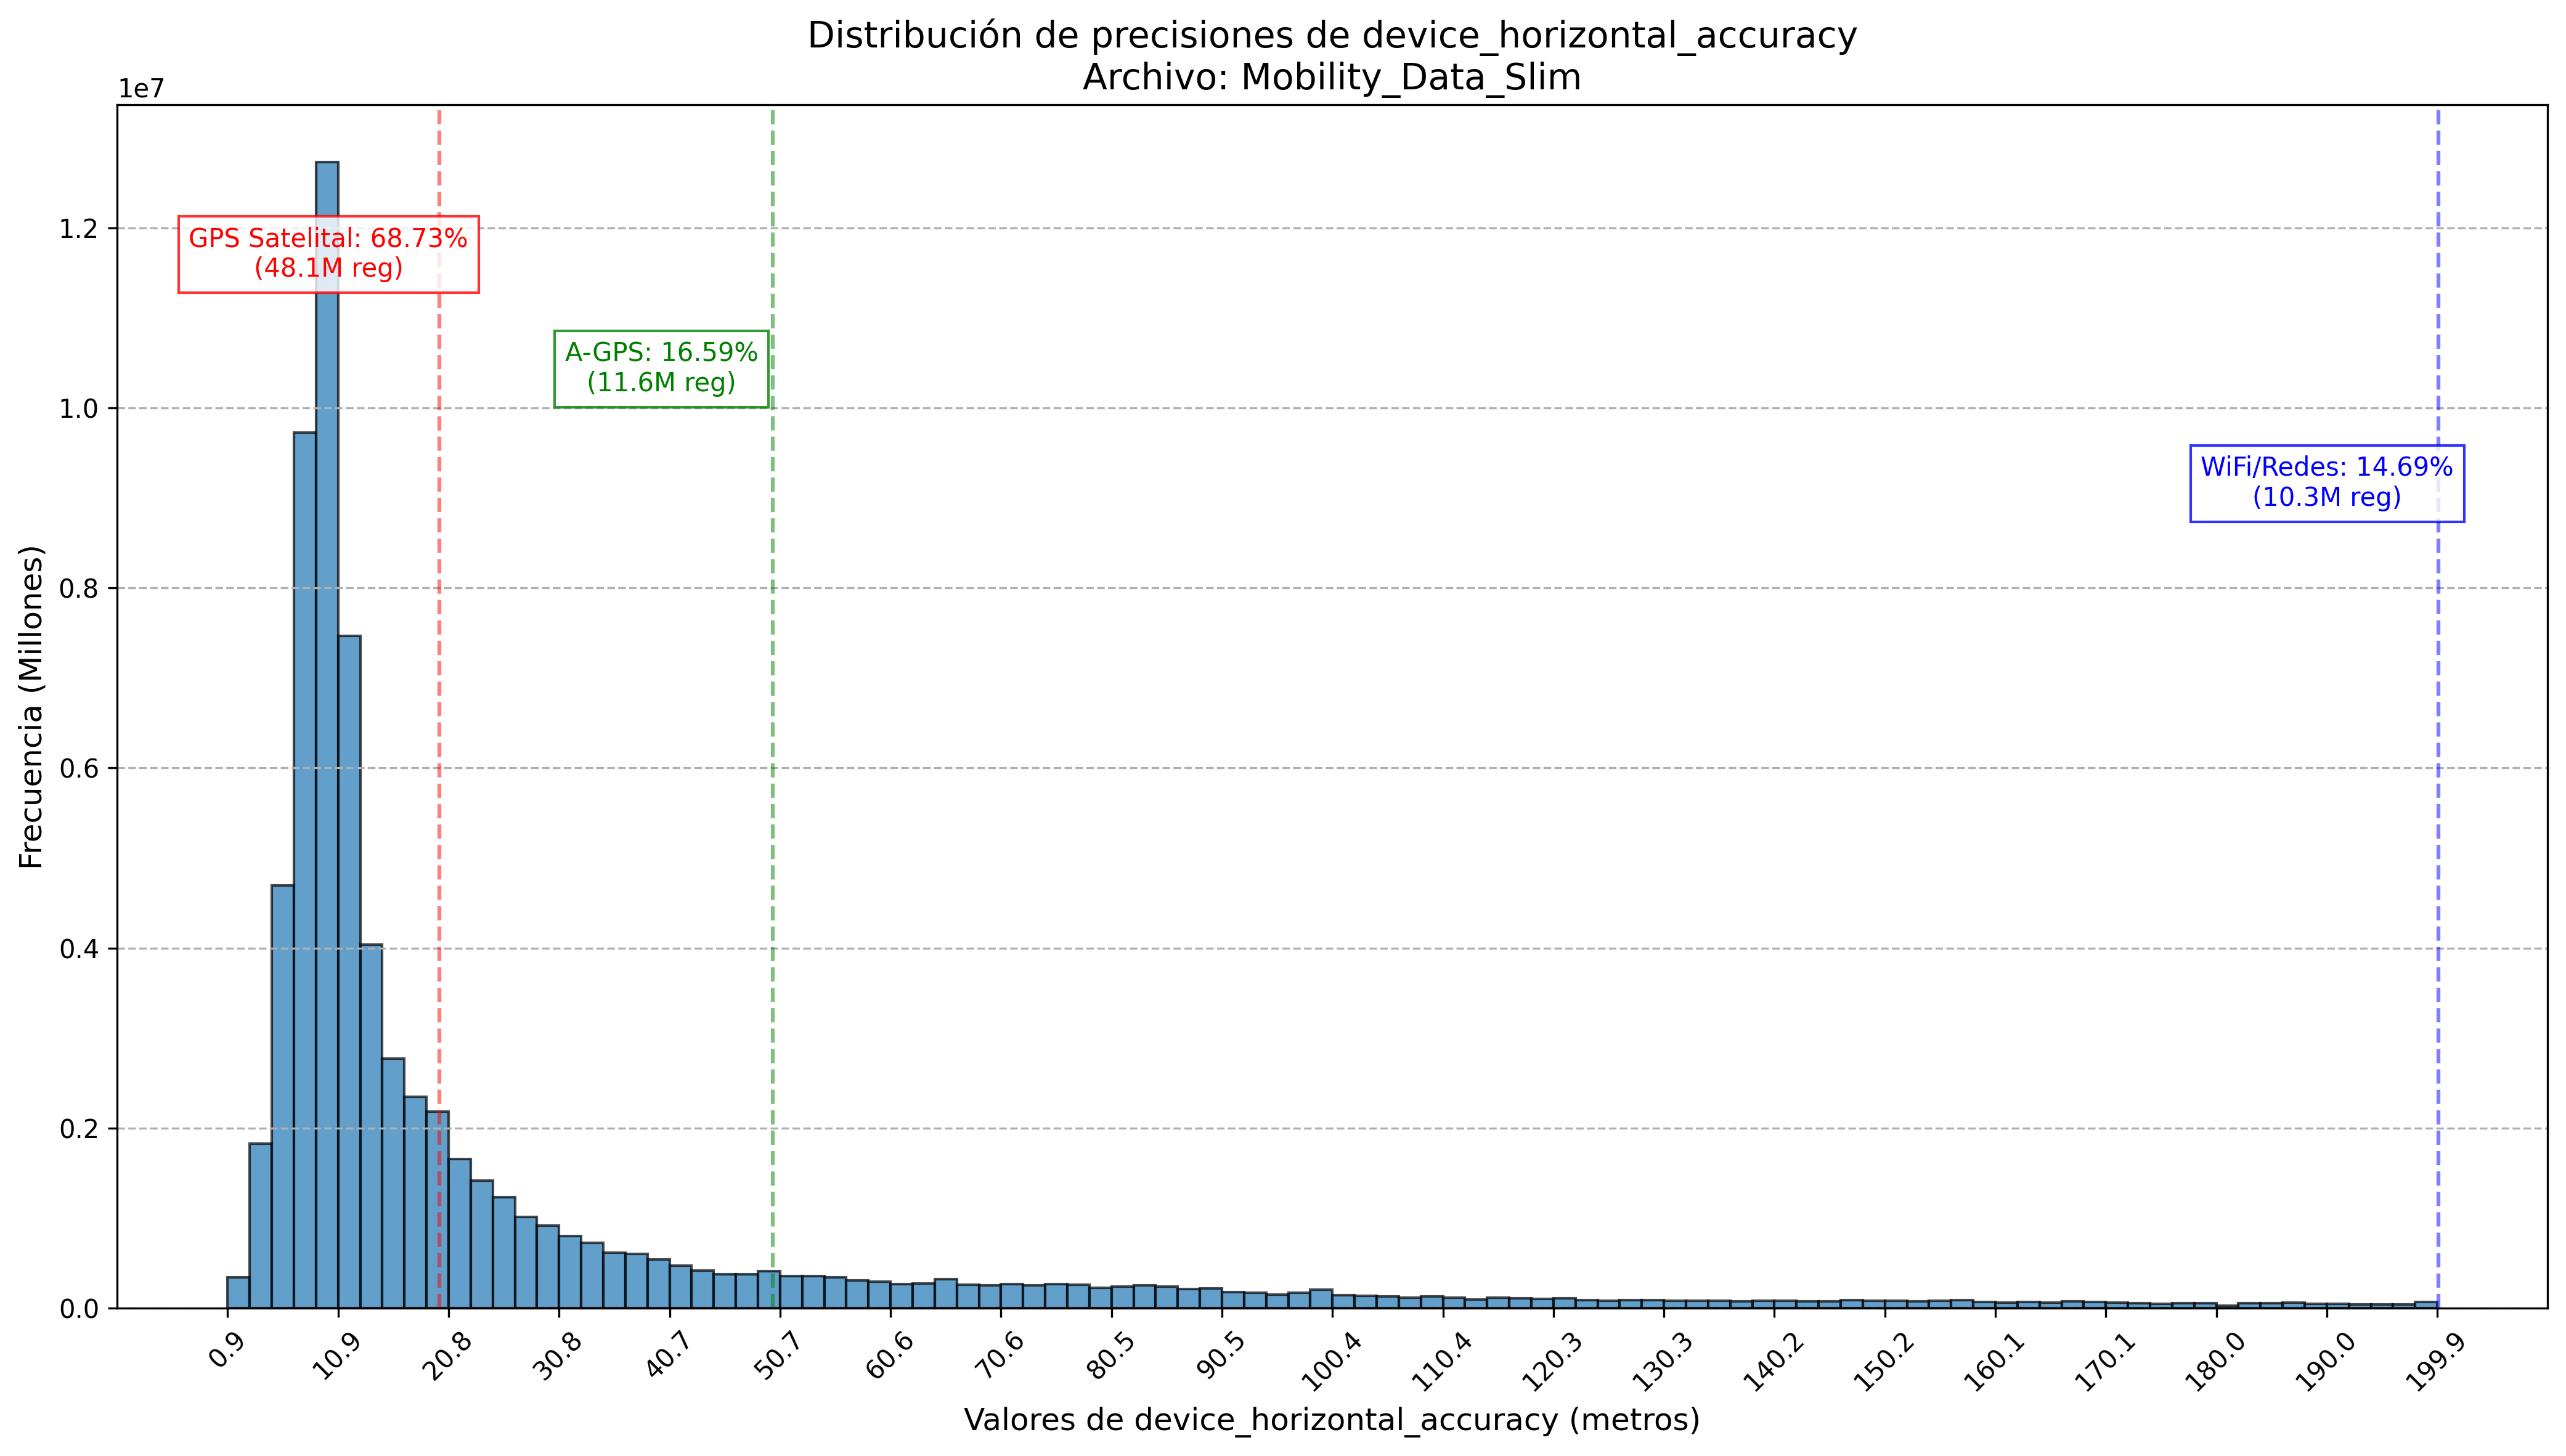
\includegraphics[width=\textwidth]{img/histograma_device_horizontal_accuracy_Mobility_Data_Slim.png}
    \caption{Frecuencia de aparación de los valores de 'device\_horizontal\_accuracy'.}
    \label{fig:accuracy_histogram}
\end{figure}

Para el objetivo de este proyecto, se busca que la configuración del GPS sea lo más precisa posible, por lo que aquellos que estén dentro del rango del GPS puro (1-20 metros) son los más relevantes. Como se puede ver en la Figura \ref{fig:accuracy_histogram}, el \textbf{68.73\%} de los valores se encuentran dentro de este rango. Sin embargo, el \textbf{31.27\%} de registros con están por encima de este rango, precisión A-GPS (5-50 metros) y triangulación por WiFi/red móvil (20-500 metros).\\
\\
La siguiente columna a evaluar es \texttt{identifier}, corresponde al identificador único de cada dispositivo.  Para analizar la frecuencia de aparición de estos valores se empleó un script que agrupa las repeticiones por rangos y grafica la cantidad de valores únicos usando escala logarítmica (ver Apéndice \ref{cod:identifier_histogram}).

\begin{figure}[H]
    \centering
    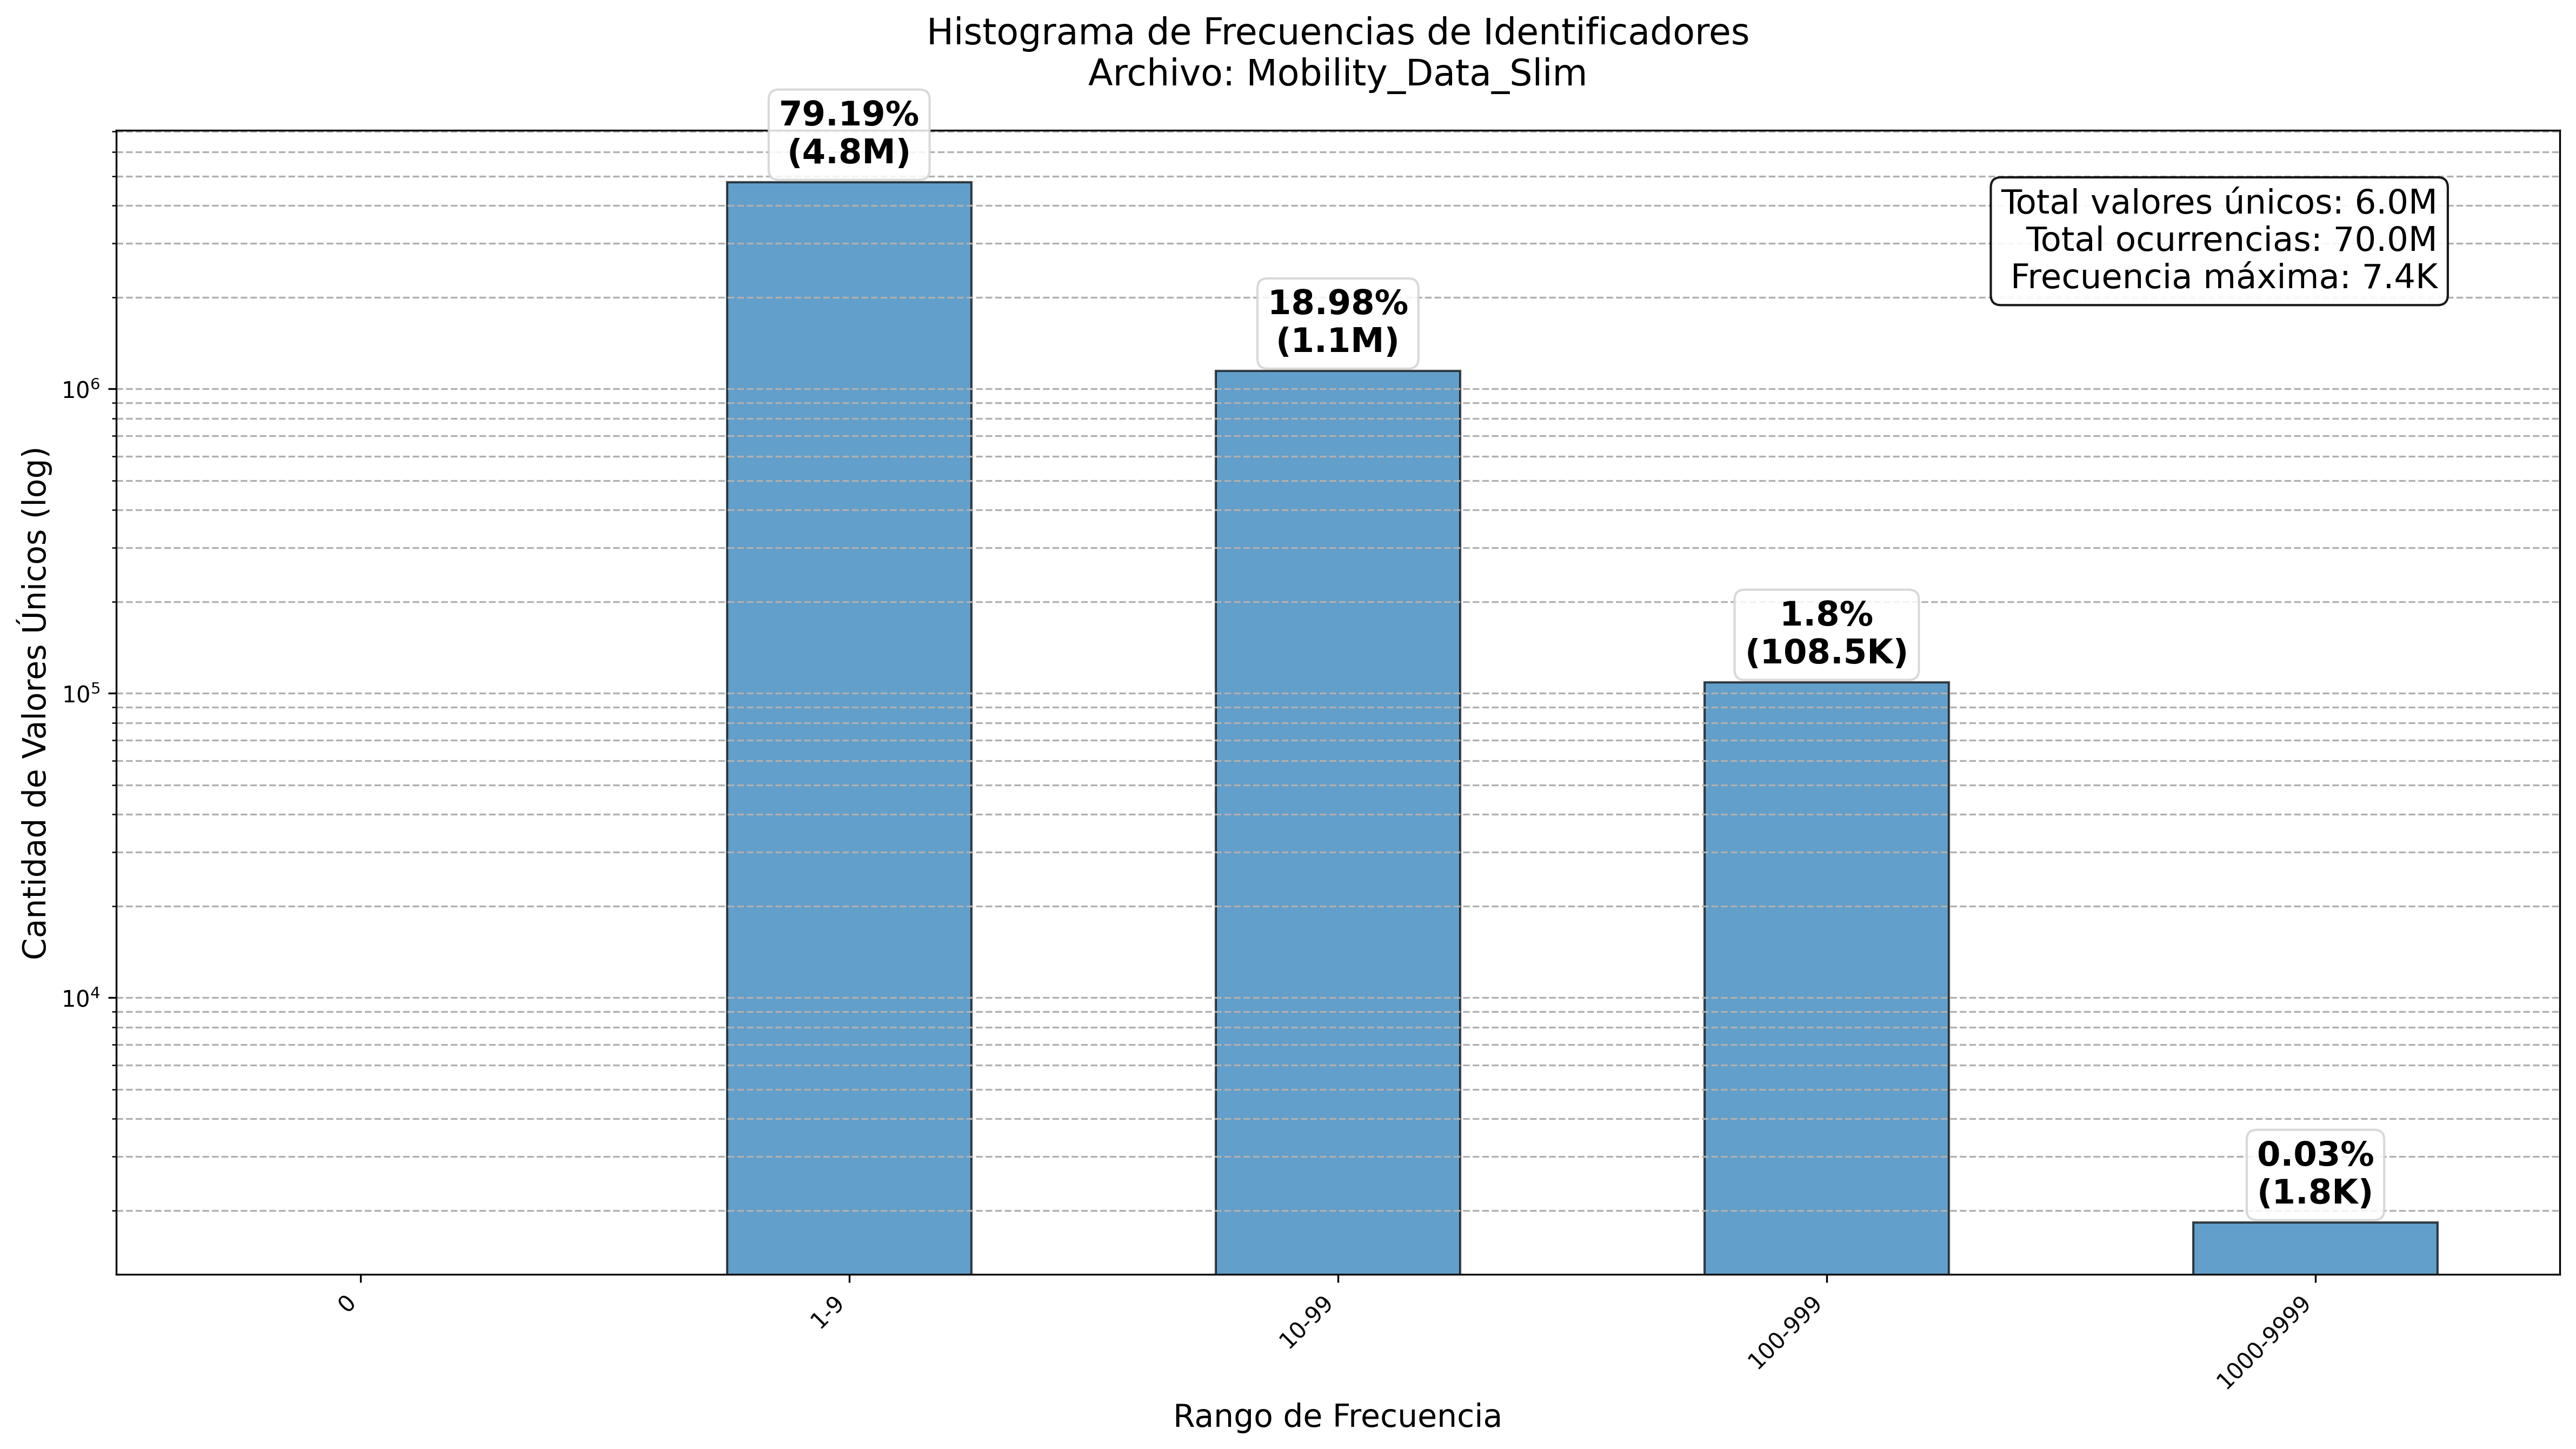
\includegraphics[width=0.8\textwidth]{img/histograma_identifier_Mobility_Data_Slim.png}
    \caption{Frecuencia de aparición de los identificadores únicos.}
    \label{fig:identifier_histogram}
\end{figure}

 De este script sabemos que el total de individuos es de \textbf{6,022,772} de los cuales el \textbf{79.19\%} tienen una frecuencia de aparición de una a nueve veces, esto es \textbf{4,769,317} de individuos. Así mismo de la Figura \ref{fig:identifier_histogram} podemos observar que hay poco más de un \textbf{20\%} de individuos con más de 99 repeticiones. Por lo que se necesita hacer un análisis más detallado, para ello se ejecuta el código del Apéndice \ref{cod:identifier_histogram_detailed}, el cual segmenta los datos en tres rangos: 1-99, 100-1000 y 1001-10000 repeticiones.

\begin{figure}[htbp]
    \centering
    \begin{subfigure}[t]{0.48\textwidth-1em}
        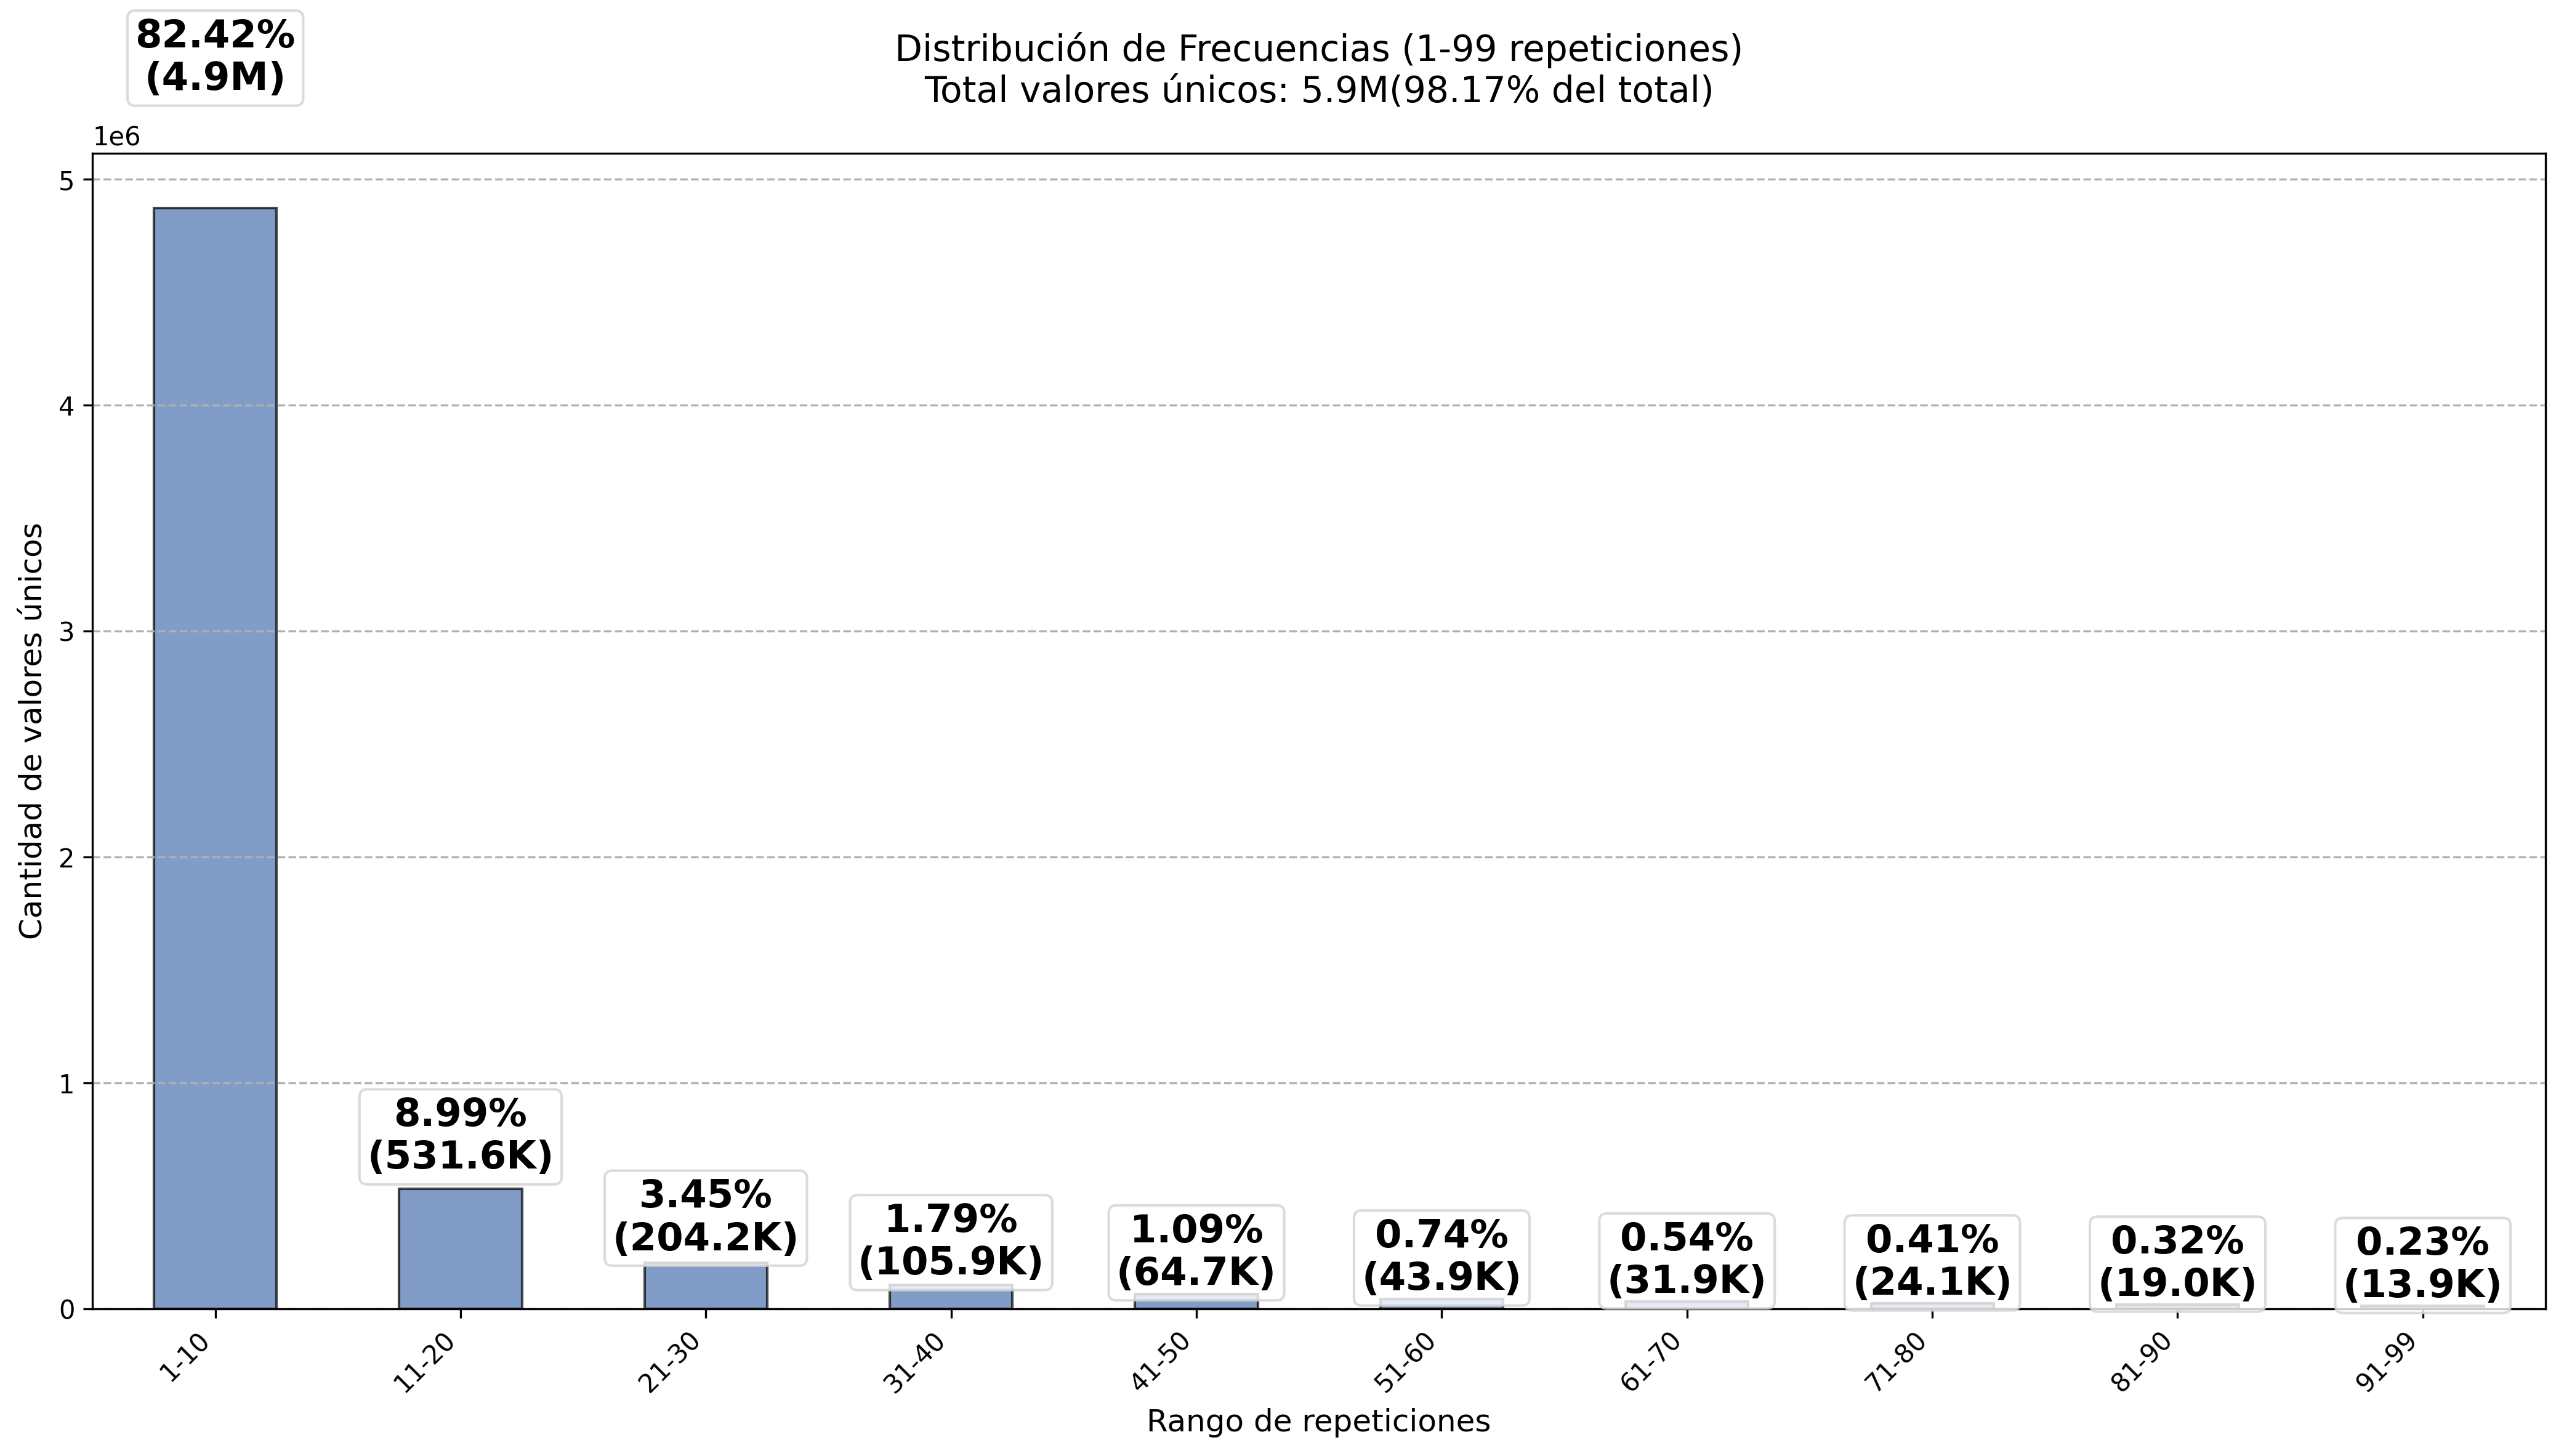
\includegraphics[width=\linewidth]{img/histograma_1-99_identifier_Mobility_Data_Slim.png}
        \caption{Histograma 1-99 repeticiones}
        \label{fig:sub1}
    \end{subfigure}
    \hfill
    \begin{subfigure}[t]{0.48\textwidth-1em}
        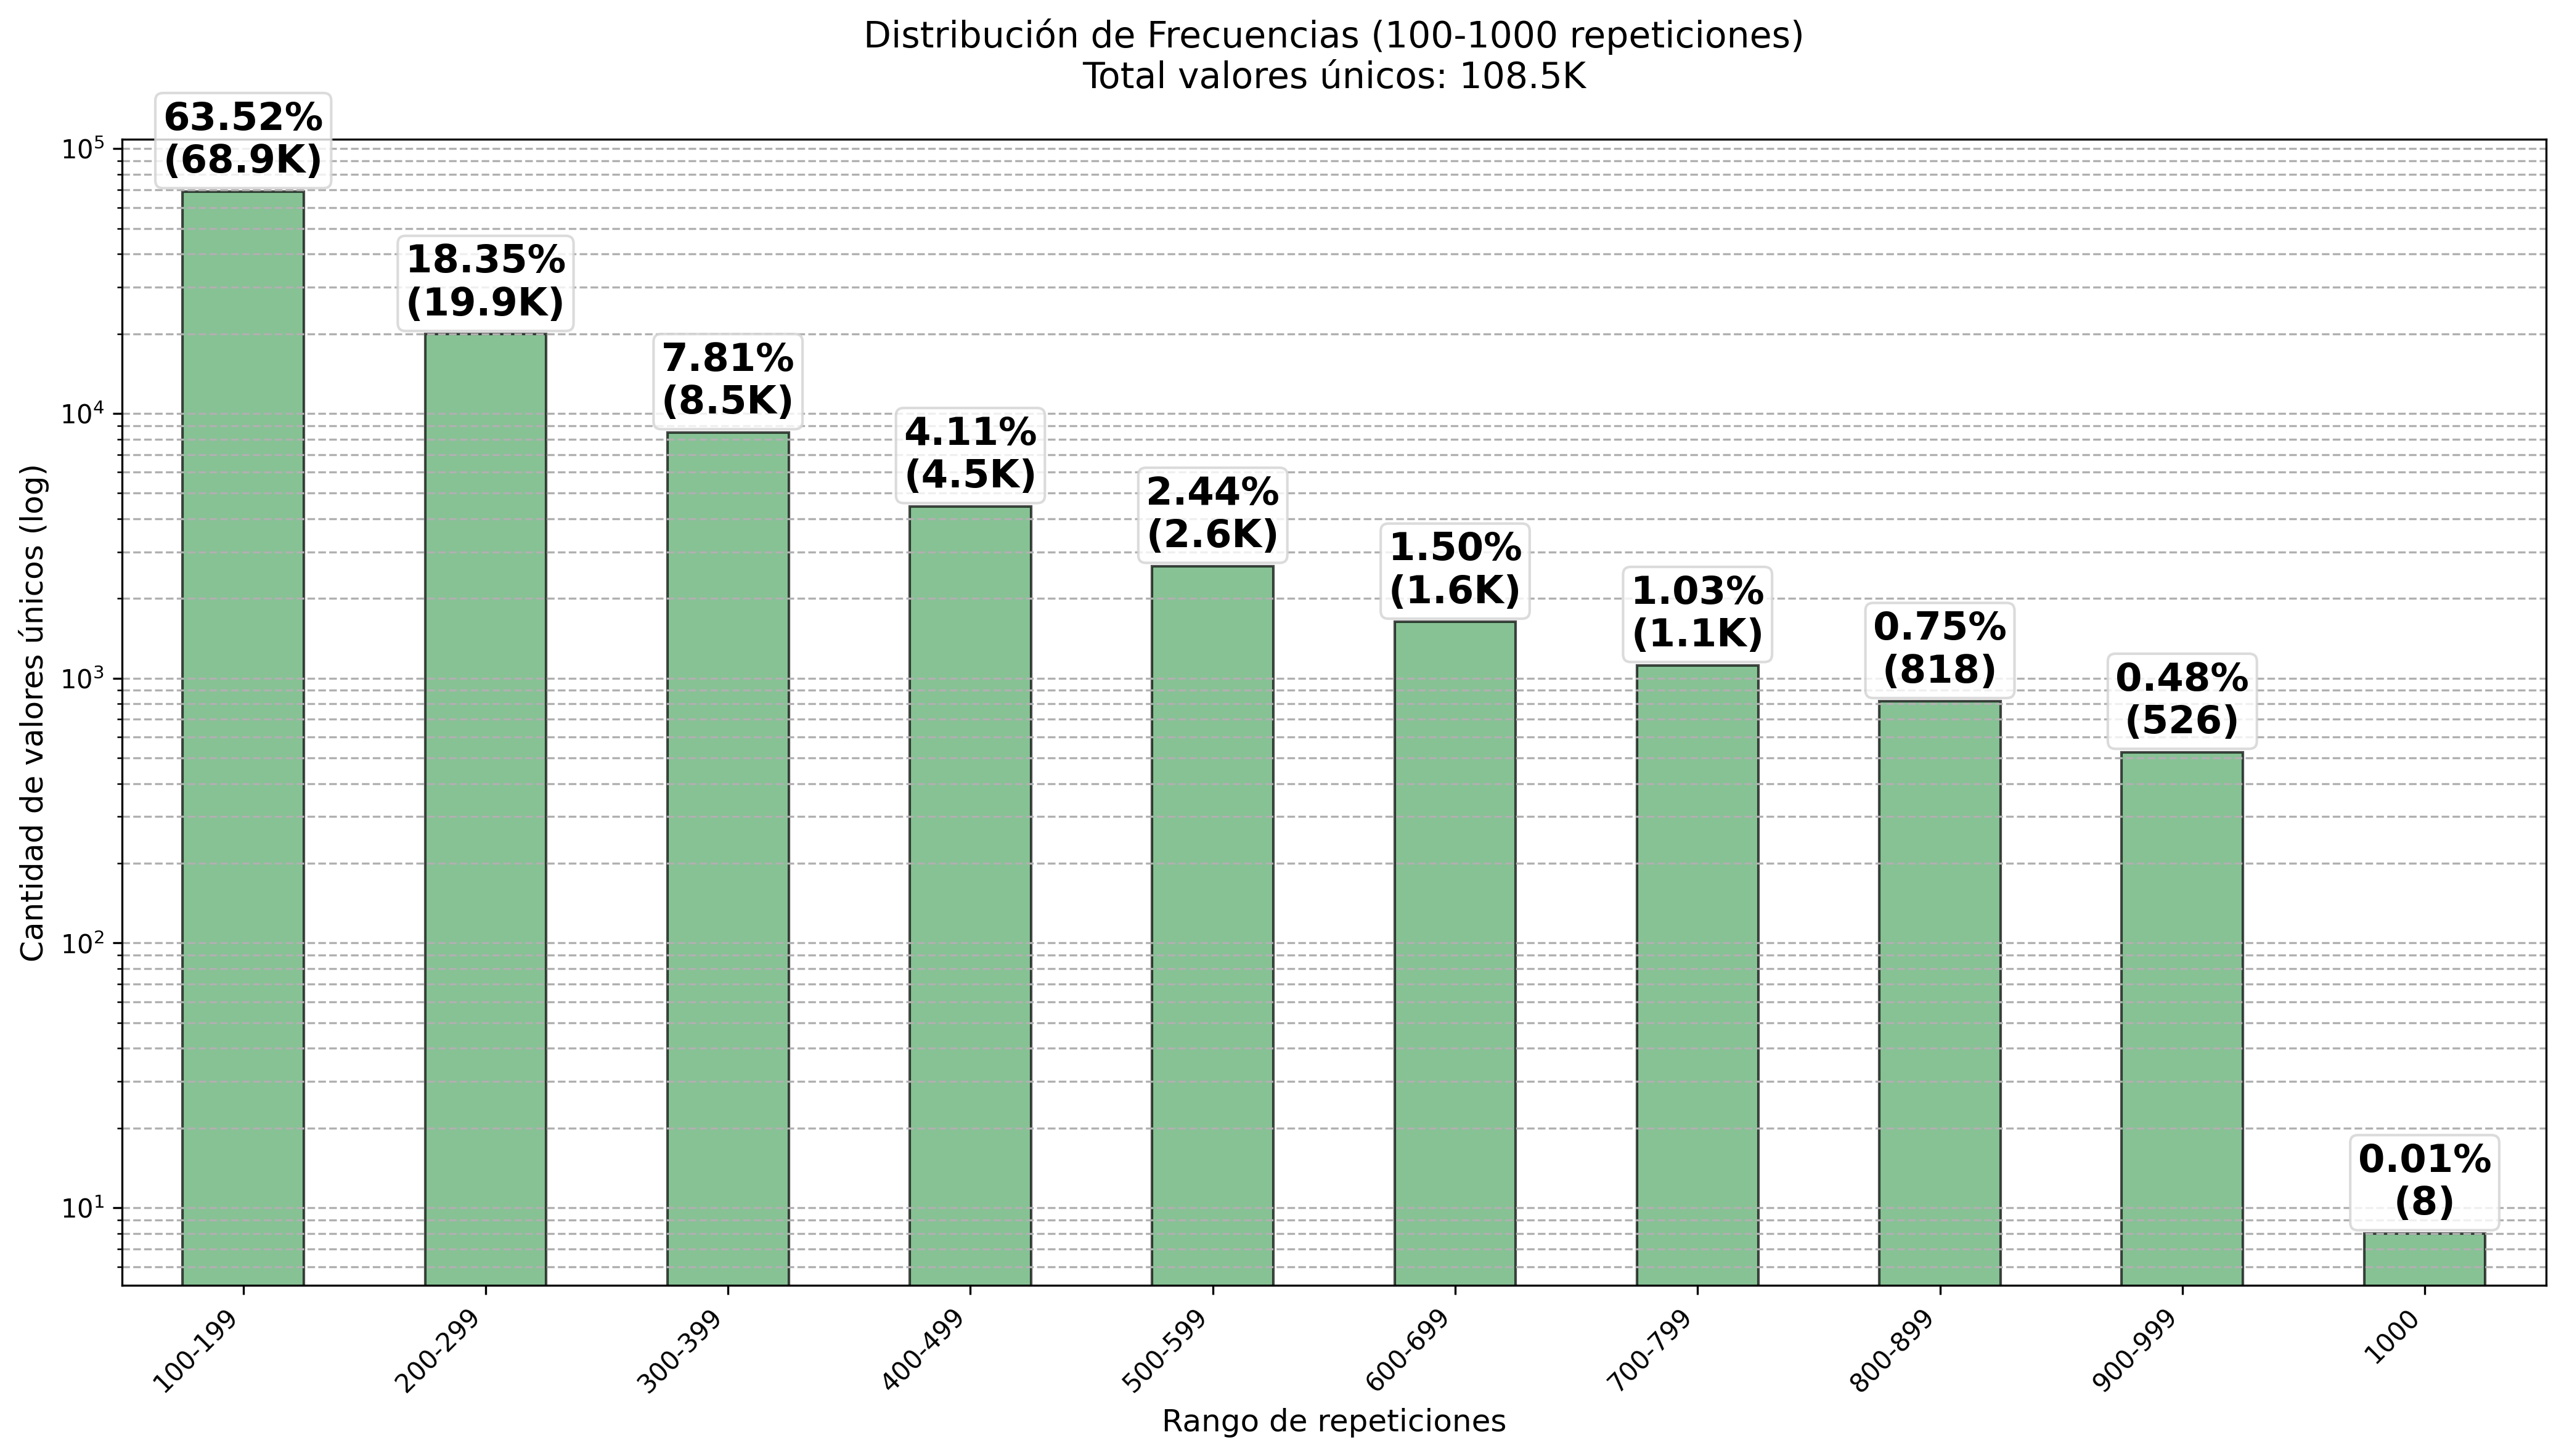
\includegraphics[width=\linewidth]{img/histograma_100-1k_identifier_Mobility_Data_Slim.png}
        \caption{Histograma 100–1000 repeticiones}
        \label{fig:sub2}
    \end{subfigure}

    \vspace{0.5cm}

    \begin{subfigure}[t]{0.48\textwidth}
        \centering
        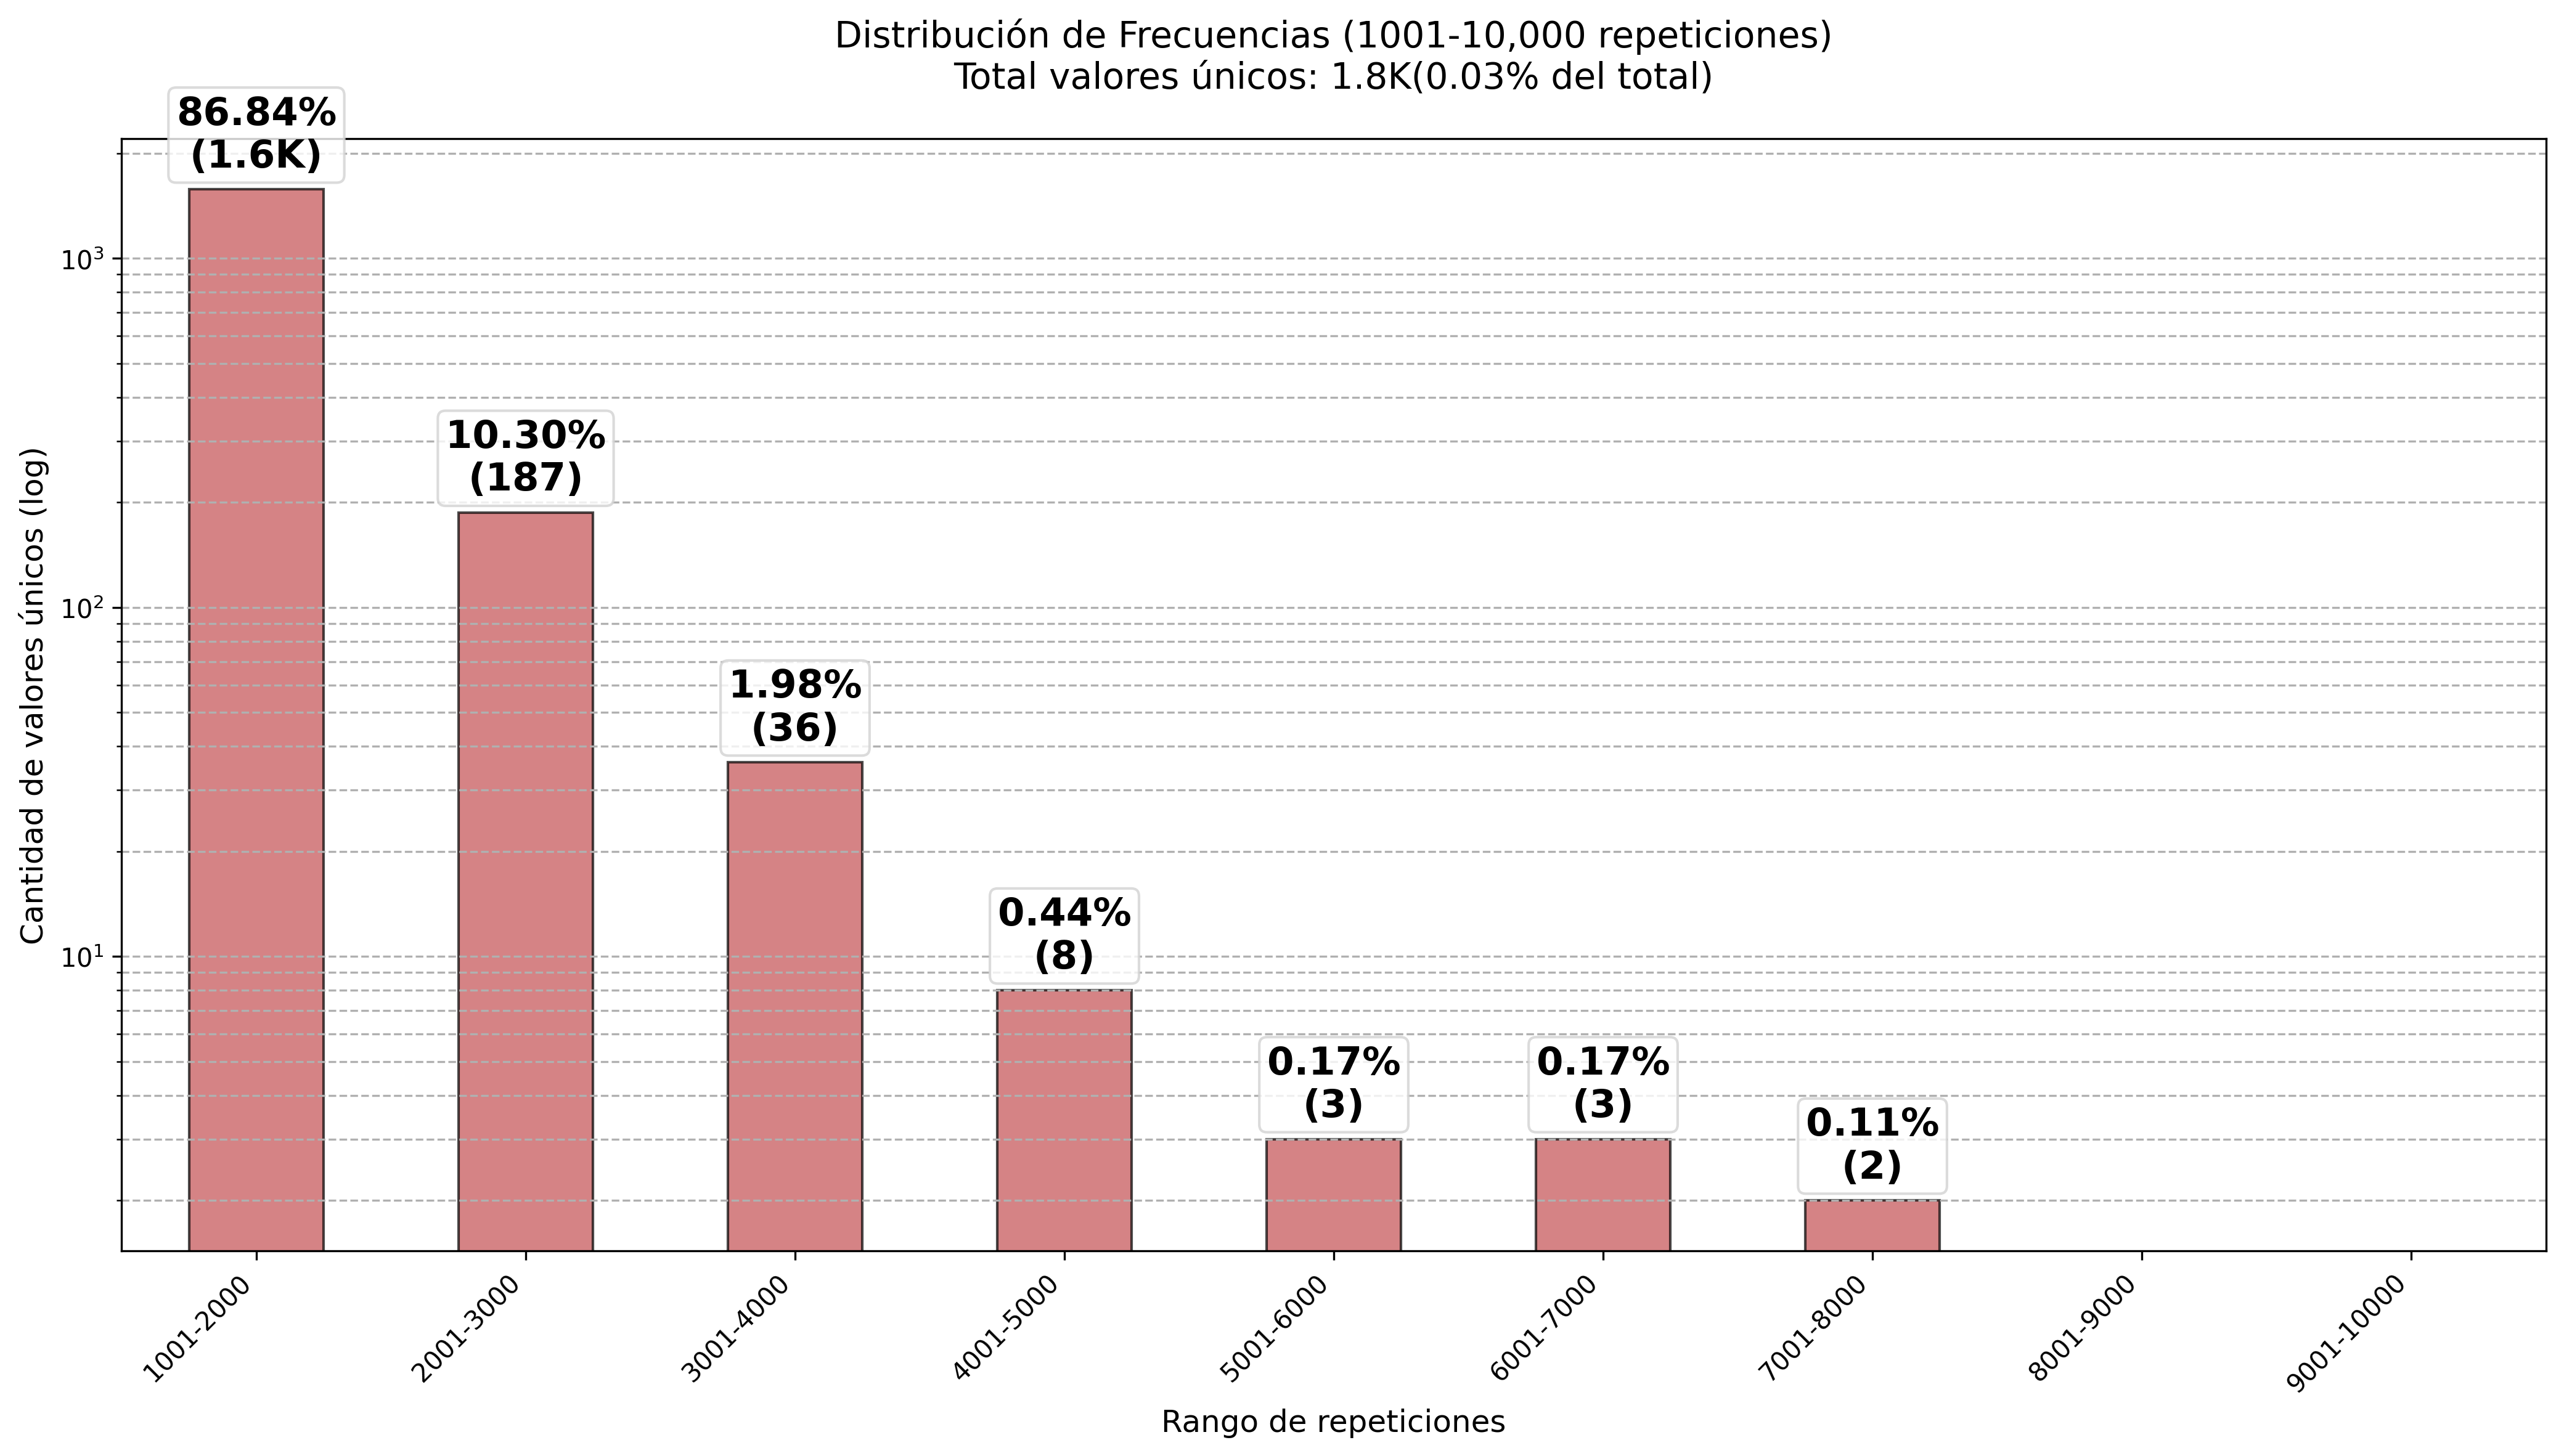
\includegraphics[width=\linewidth]{img/histograma_1k-10k_identifier_Mobility_Data_Slim.png}
        \caption{Histograma 1001–10000 repeticiones}
        \label{fig:sub3}
    \end{subfigure}

    \caption{Comparación de histogramas por rangos de repeticiones.}
    \label{fig:histogramas}
\end{figure}

Con la información obtenida de los histogramas de la figura anterior, se puede observar que el \textbf{98.17\%} de los identificadores únicos tienen entre 1 y 99 repeticiones, lo que equivale a \textbf{5,912,437} individuos. Por otro lado, el \textbf{1.83\%} restante tiene entre 100 y 10,000 repeticiones, lo que equivale a \textbf{110,335} individuos. Con base en esta información aún no se puede determinar que registros eliminar. Por lo que ahora se eliminarán aquellos registros que sean duplicados, es decir, aquellos que tengan el mismo 
\texttt{identifier}, \texttt{timestamp}, \texttt{device\_lat} y \texttt{device\_lon}. Para ello se utilizó el código del Apéndice \ref{cod:csv_deduplicate}, que elimina los duplicados y genera un nuevo archivo CSV con los registros de individuos. \\
Con este nuevo archivo se vuelve a realizar el análisis de frecuencia de aparición de individuos. En la siguiente figura se muestra el histograma de la frecuencia de aparición de los identificadores únicos

\begin{figure}[H]
    \centering
    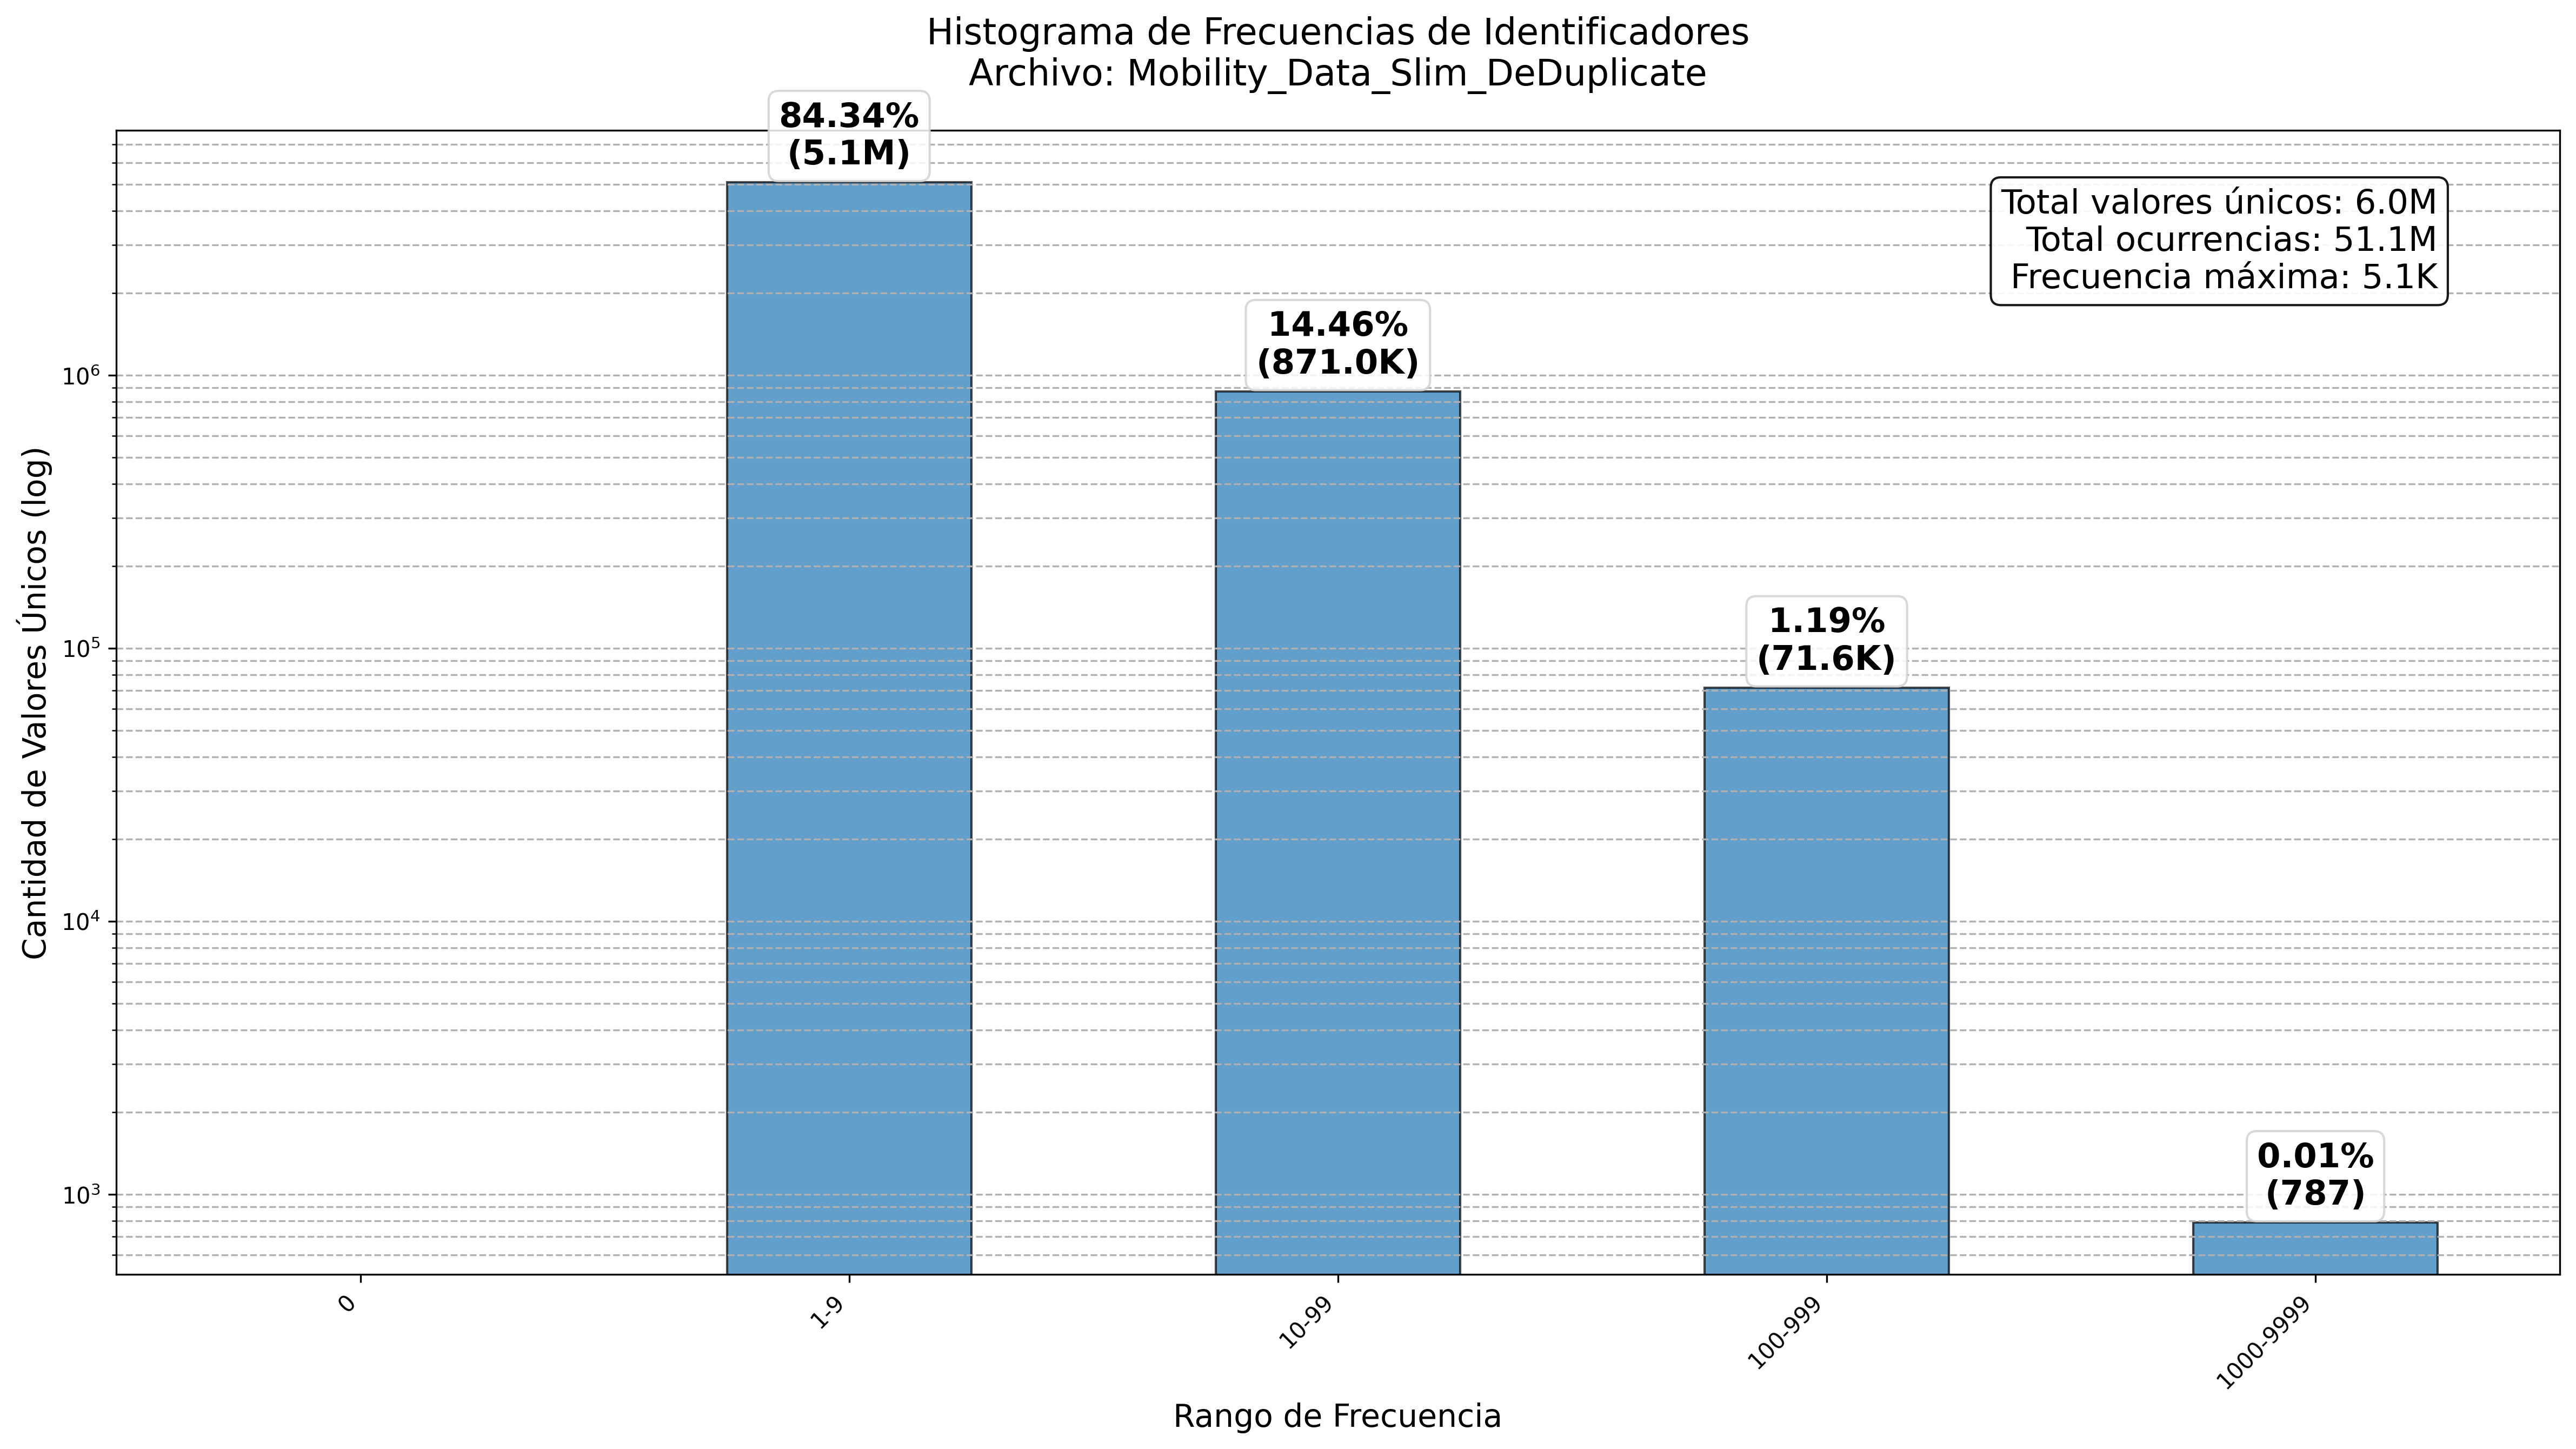
\includegraphics[width=0.8\textwidth]{img/histograma_identifier_Mobility_Data_Slim_DeDuplicate.png}
    \caption{Frecuencia de aparición de los identificadores únicos después de eliminar duplicados.}
    \label{fig:identifier_histogram_deduplicate}
\end{figure}

Comparando los resultados de la Figura \ref{fig:identifier_histogram} y la Figura \ref{fig:identifier_histogram_deduplicate} podemos destacar varios hallazgos importantes: 

\begin{description}
    \item[Preservación de la diversidad de individuos]: Los \textbf{6,022,772} únicos se mantuvieron sin cambios.
    \item[Reducción de redundancias]: La eliminación del \textbf{27\%} de registros. De \textbf{70 millones} a \textbf{51 millones} de registros.
    \item[Correcció de sesgos]: La reducción del \textbf{31.1\%} en la frecuencia máxima de aparición (de 7,400 a 5,100) corrige sesgos que afectaban especialmente a individuos con alta frecuencia de registros repetidos. 
\end{description}

Como podemos ver la Figura \ref{fig:histogramasDeDuplicate} la distribución de los individuos se mantiene similar; sin embargo, el \textbf{98.8\%} de los identificadores únicos tienen entre 1 y 99 repeticiones, lo que equivale a \textbf{5,950,336} individuos. Por otro lado, el \textbf{1.2\%} restante tiene entre 100 y 10,000 repeticiones, lo que equivale a \textbf{72,436} individuos. Con estos datos podemos concluir que la mayoría de los individuos tienen un número limitado de registros, lo que sugiere que la mayoría de los usuarios no están generando datos de manera continua o frecuente. 
Ahora bien para poder tener una mejor idea de la distribución de los individuos, se analiza la distribución de los individuos sin duplicados para cada día registrado en el conjunto de datos. Para ello se utilizó el código del Apéndice \ref{cod:identifier_histogram_daily}.

\begin{figure}[H]
    \centering
    \begin{subfigure}[t]{0.48\textwidth-1em}
        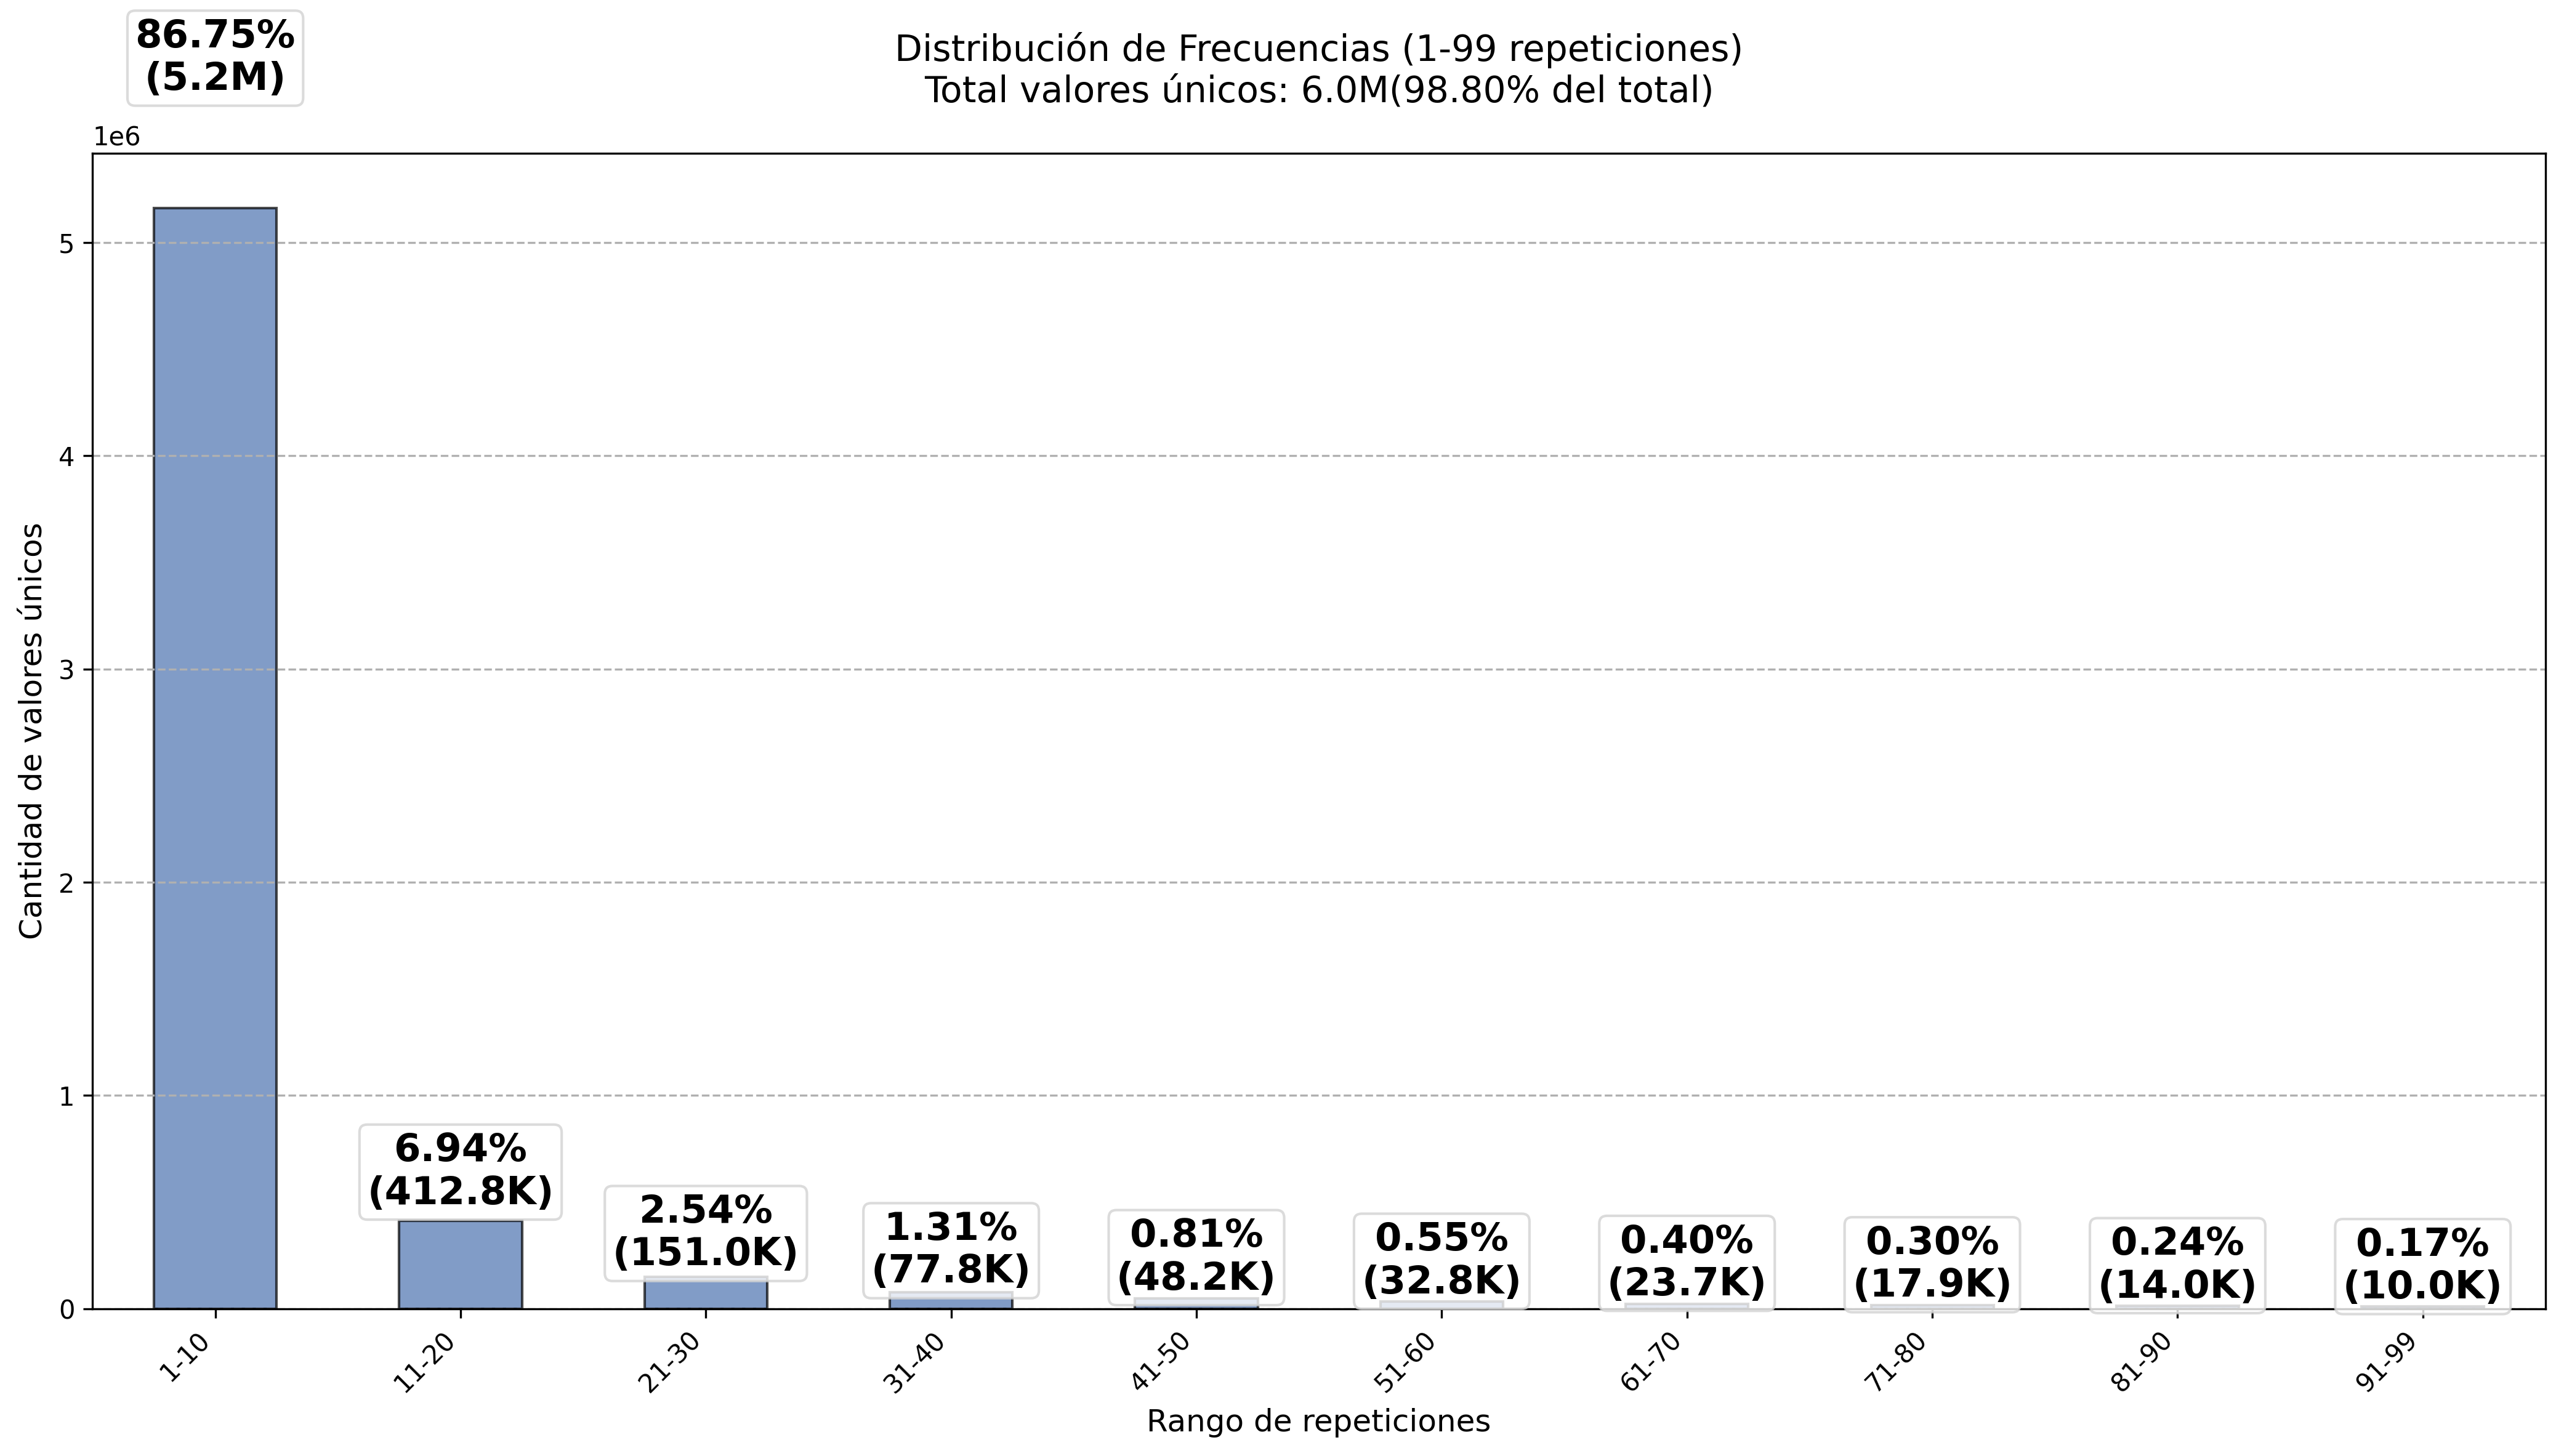
\includegraphics[width=\linewidth]{img/histograma_1-99_identifier_Mobility_Data_Slim_DeDuplicate.png}
        \caption{Histograma 1-99 repeticiones}
        \label{fig:sub1}
    \end{subfigure}
    \hfill
    \begin{subfigure}[t]{0.48\textwidth-1em}
        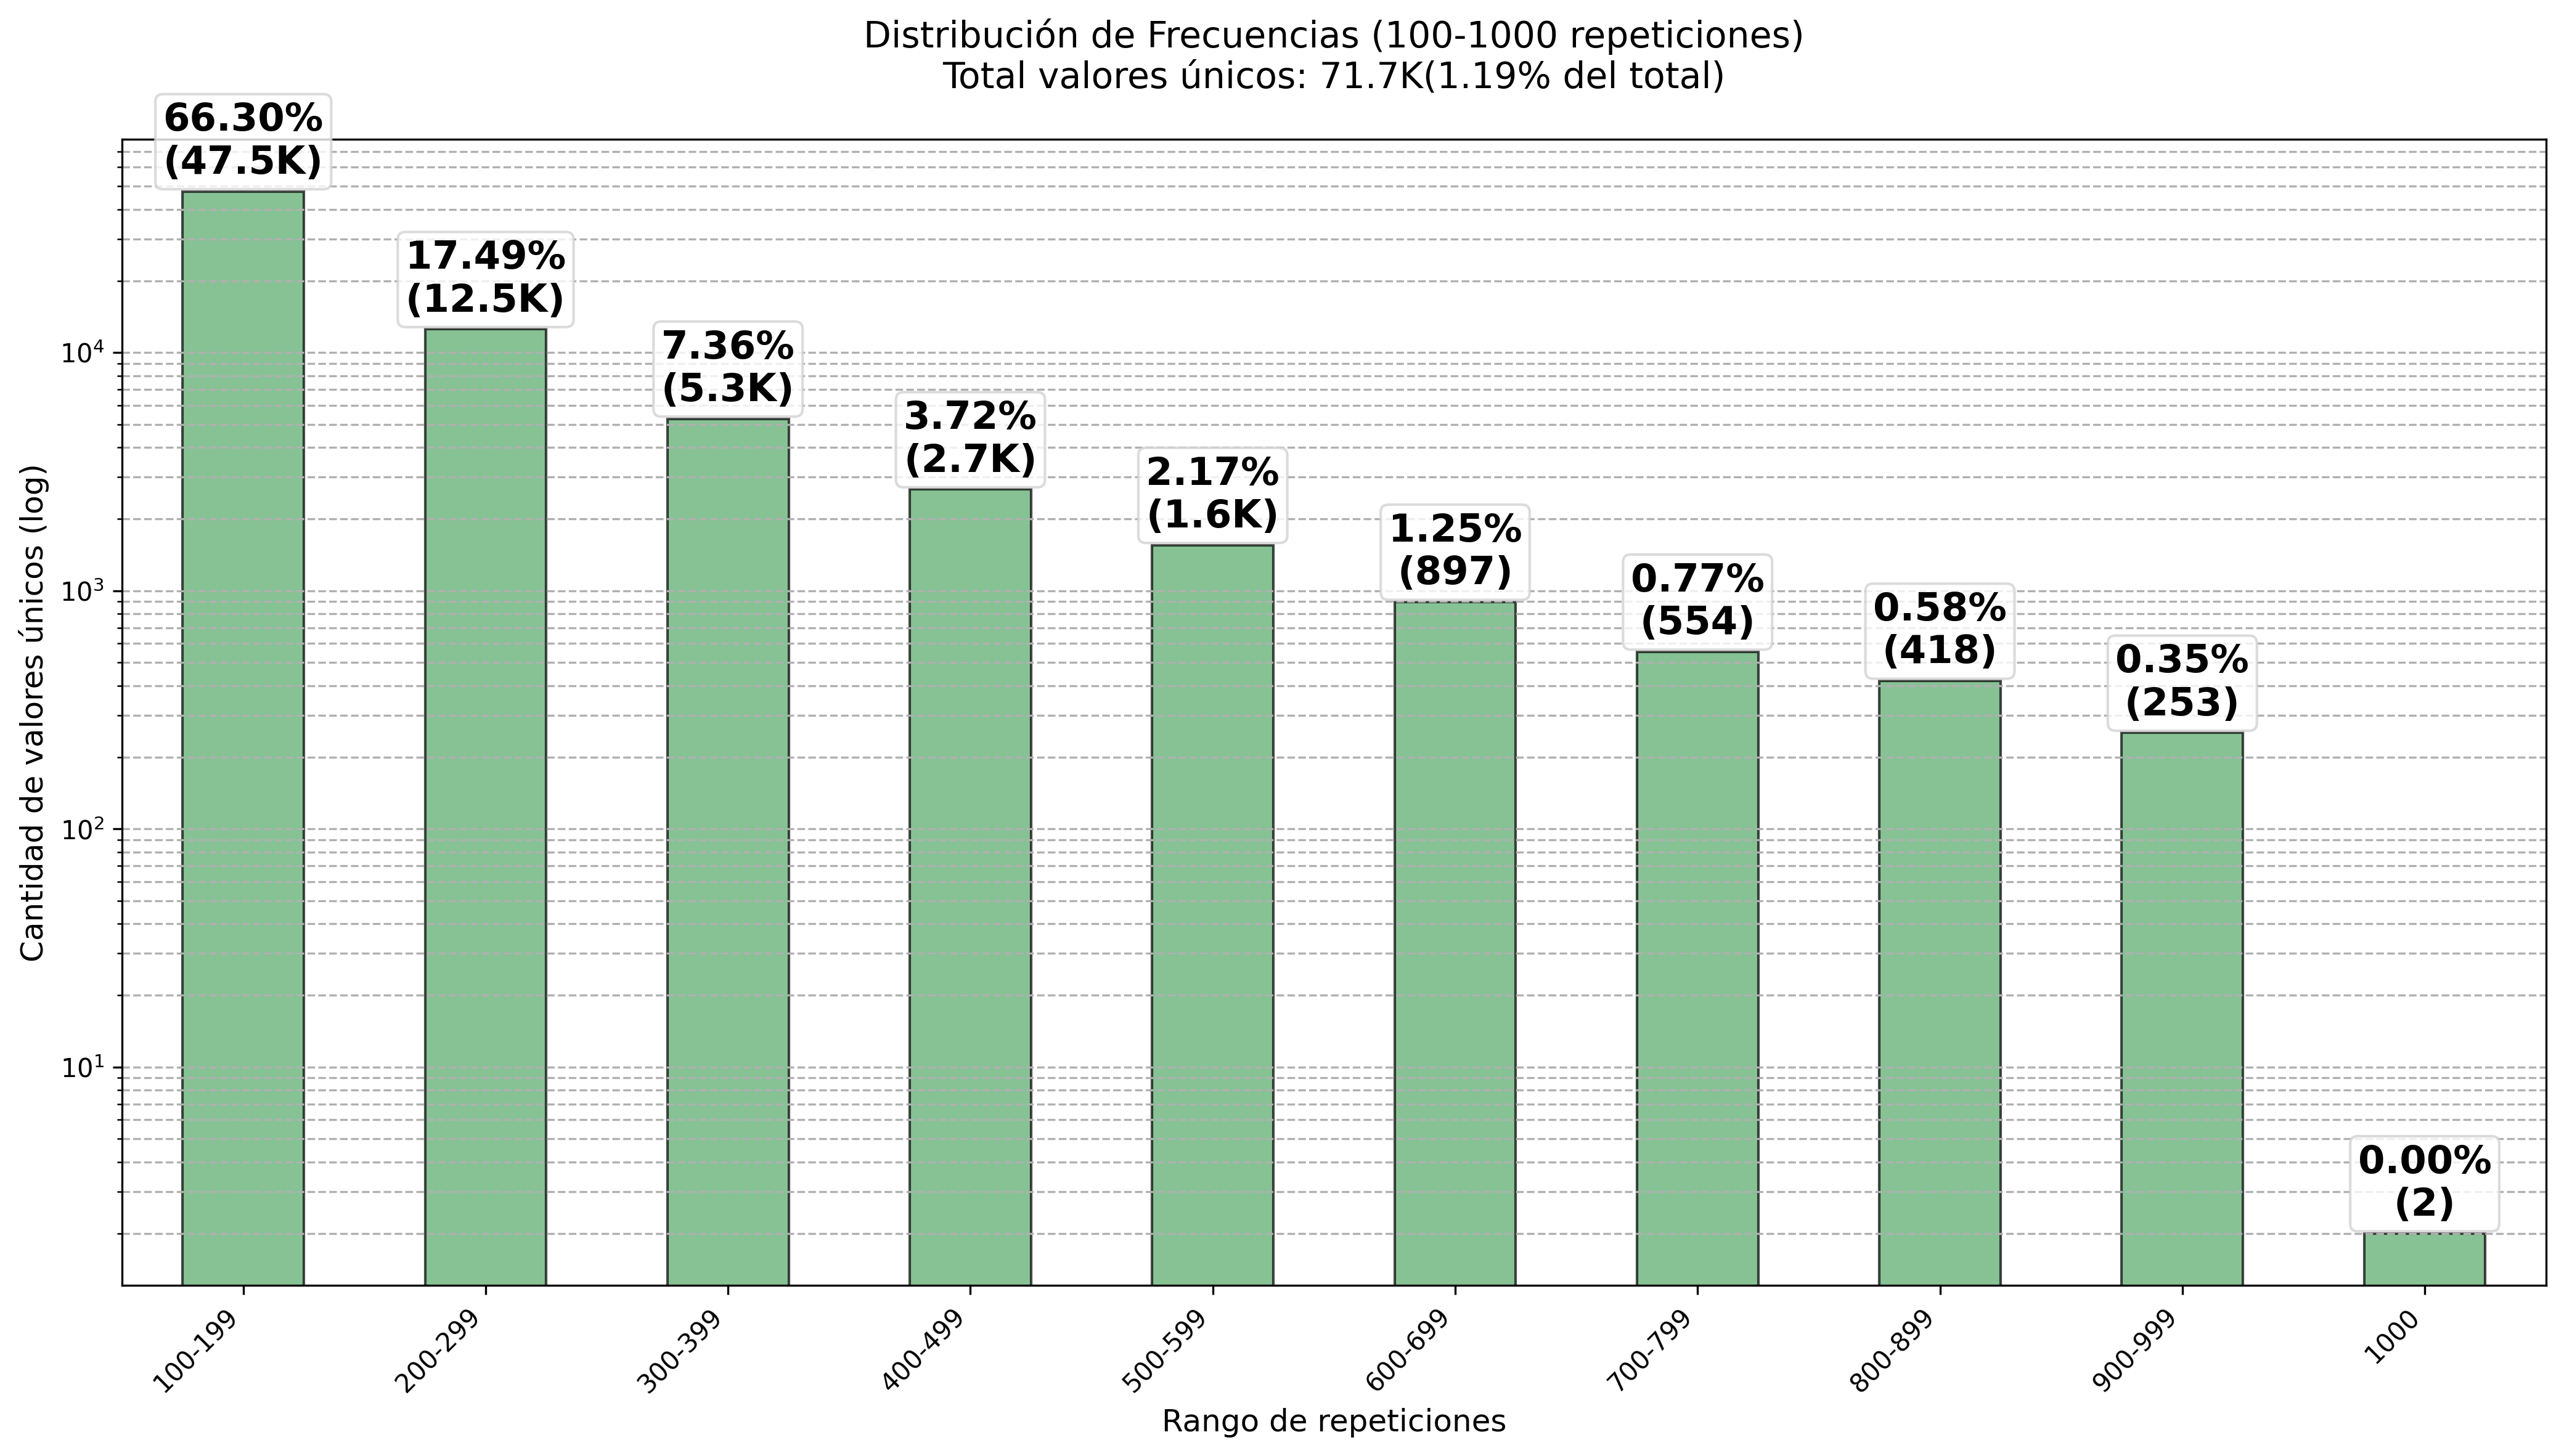
\includegraphics[width=\linewidth]{img/histograma_100-1k_identifier_Mobility_Data_Slim_DeDuplicate.png}
        \caption{Histograma 100–1000 repeticiones}
        \label{fig:sub2}
    \end{subfigure}

    \vspace{0.5cm}

    \begin{subfigure}[t]{0.48\textwidth}
        \centering
        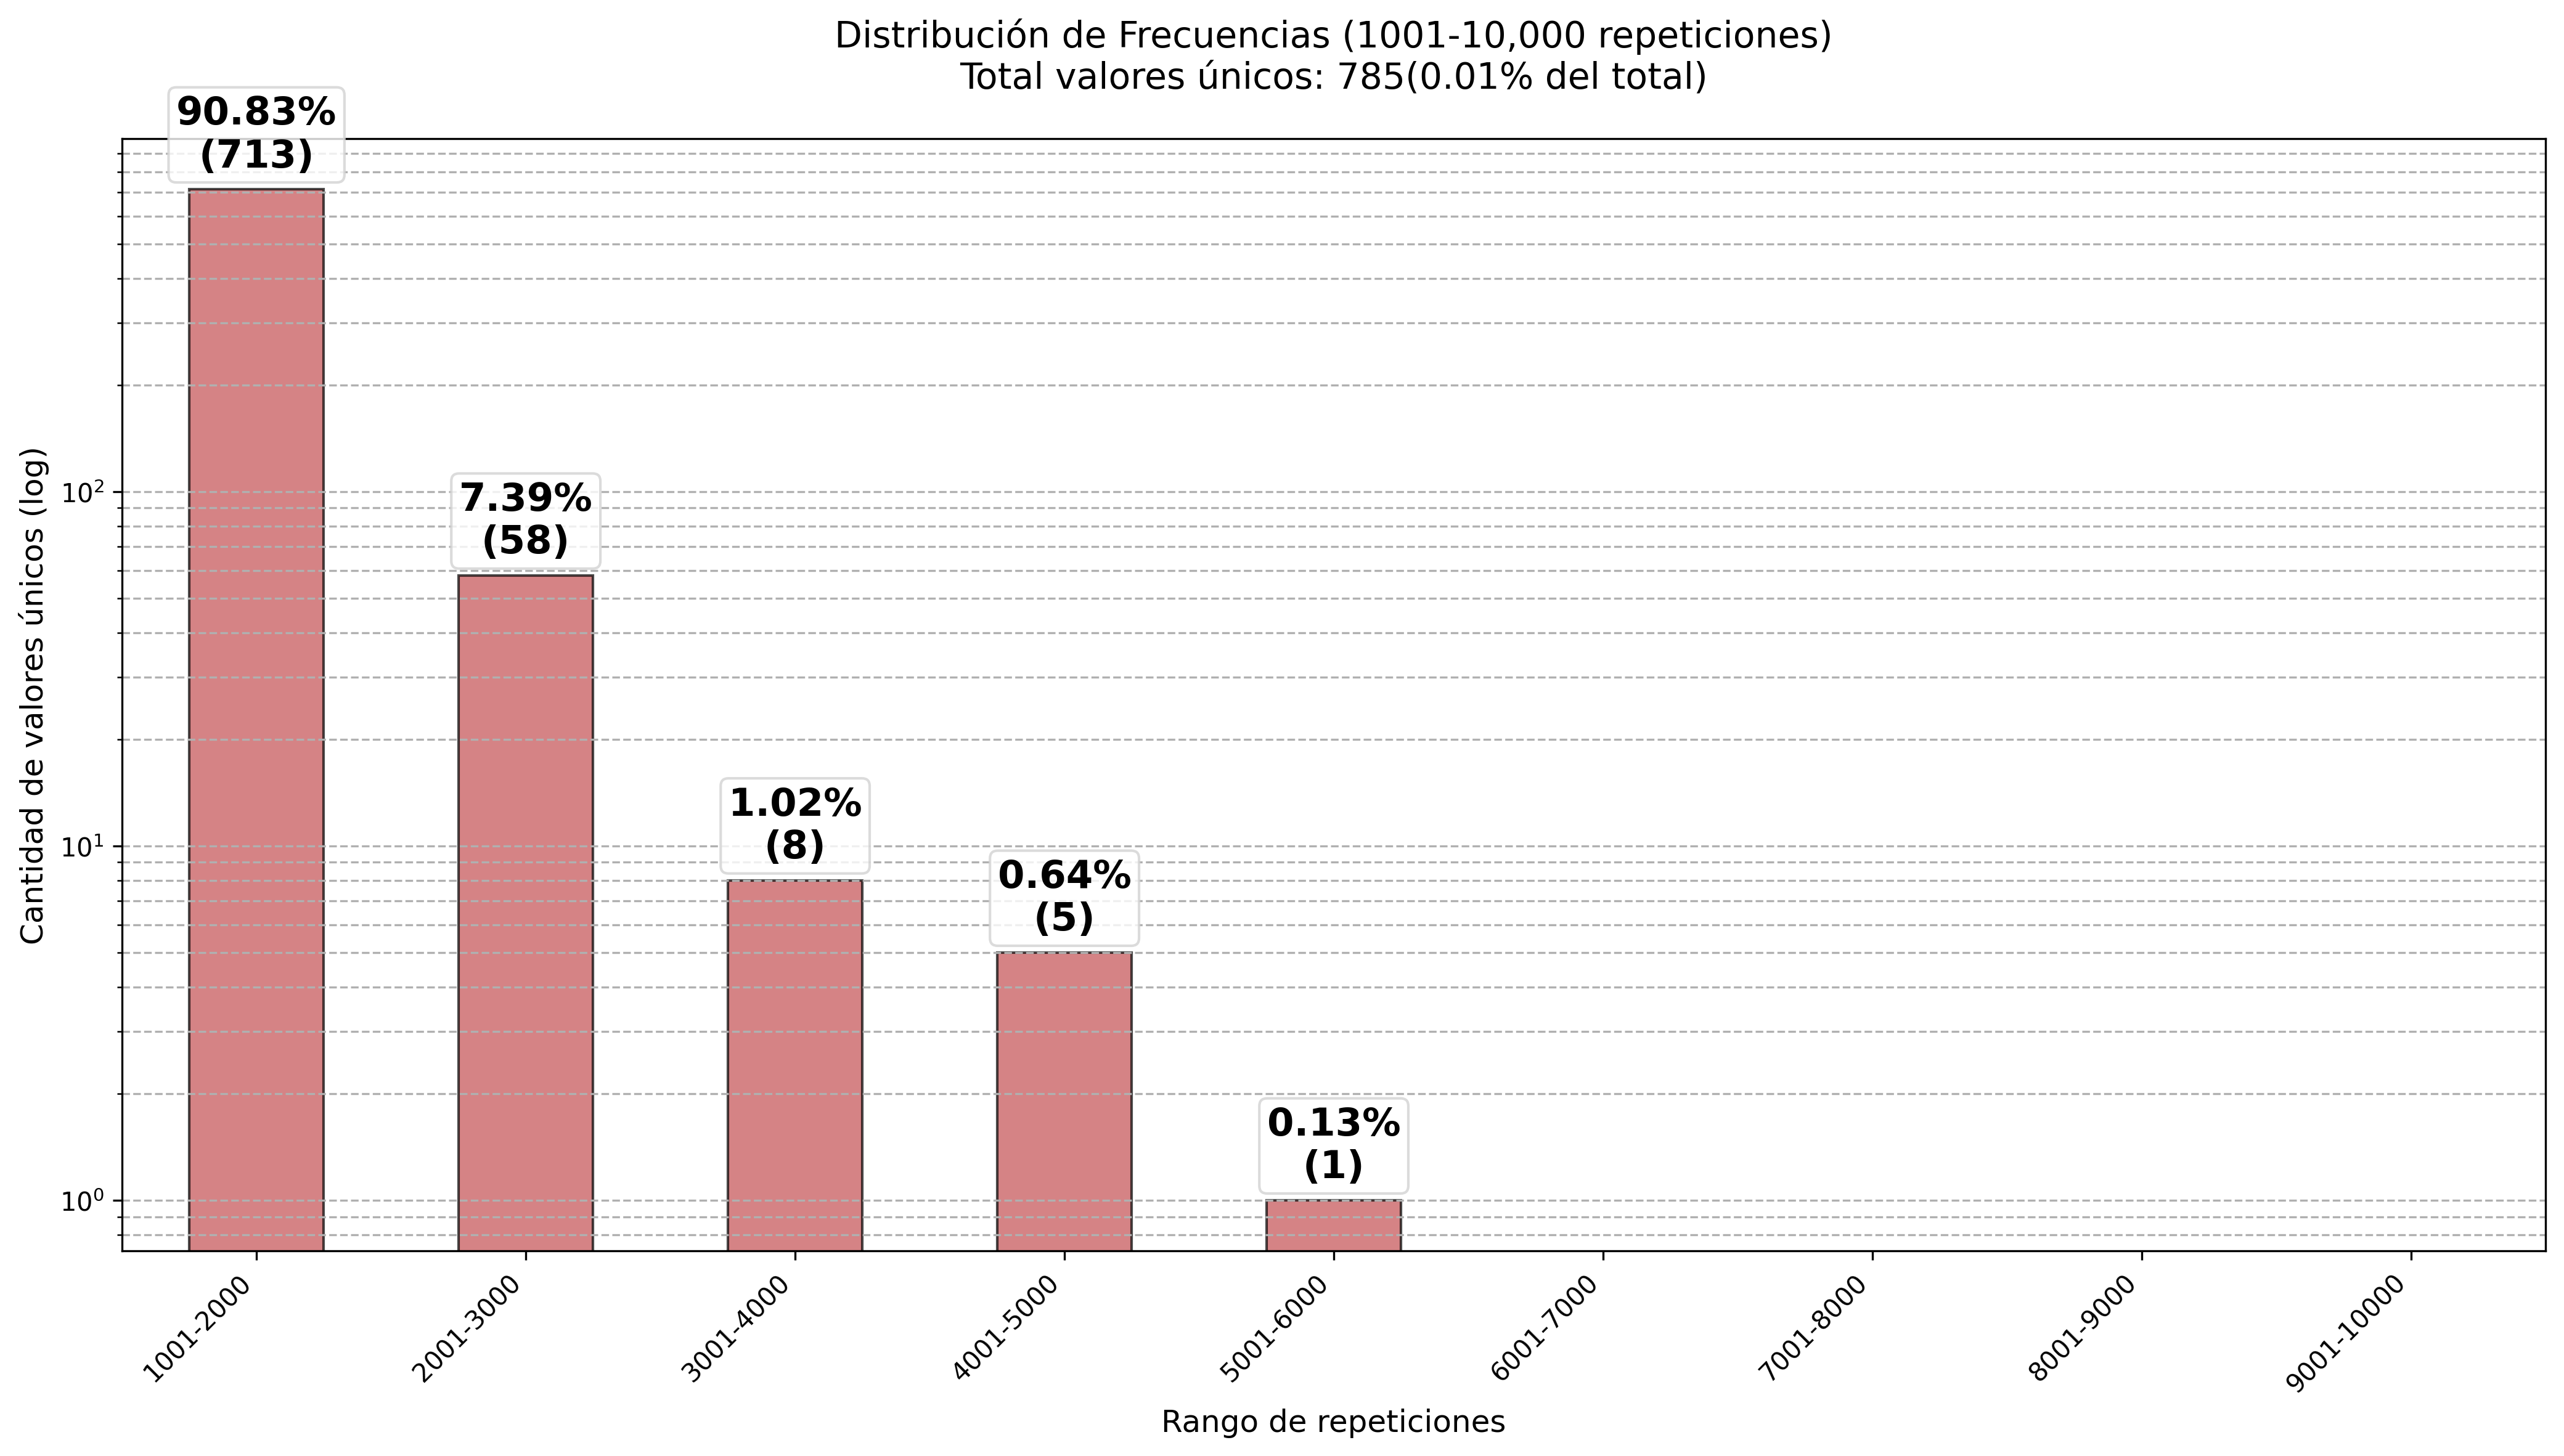
\includegraphics[width=\linewidth]{img/histograma_1k-10k_identifier_Mobility_Data_Slim_DeDuplicate.png}
        \caption{Histograma 1001–10000 repeticiones}
        \label{fig:sub3}
    \end{subfigure}

    \caption{Comparación de histogramas por rangos de repeticiones.}
    \label{fig:histogramasDeDuplicate}
\end{figure}

\chapter{Análisis del conjunto de datos}
% --------------------------
% ANÁLISIS DEL CONJUNTO DE DATOS DEPURADO
% --------------------------
\section{Análisis del conjunto de datos}
\label{sec:analisis_conjunto_datos}

En esta sección se presenta un análisis detallado del conjunto de datos, que incluye la identificación de patrones y tendencias en las trayectorias individuales. El conjunto de datos contiene puntos de recorrido obtenidos a lo largo de diez días. Por lo que el primer acercamiento del análisis es poder ver la distribución de los puntos de recorrido en cada día registrado por medio un histrograma por día. Para crear estos historgramas se ejecuta el código del Apéndice \ref{cod:identifier_histogram_daily}. A continuación, se muestran estos histogramas.

\begin{figure}[htbp]
    \centering
    \begin{subfigure}[t]{0.48\textwidth-1em}
        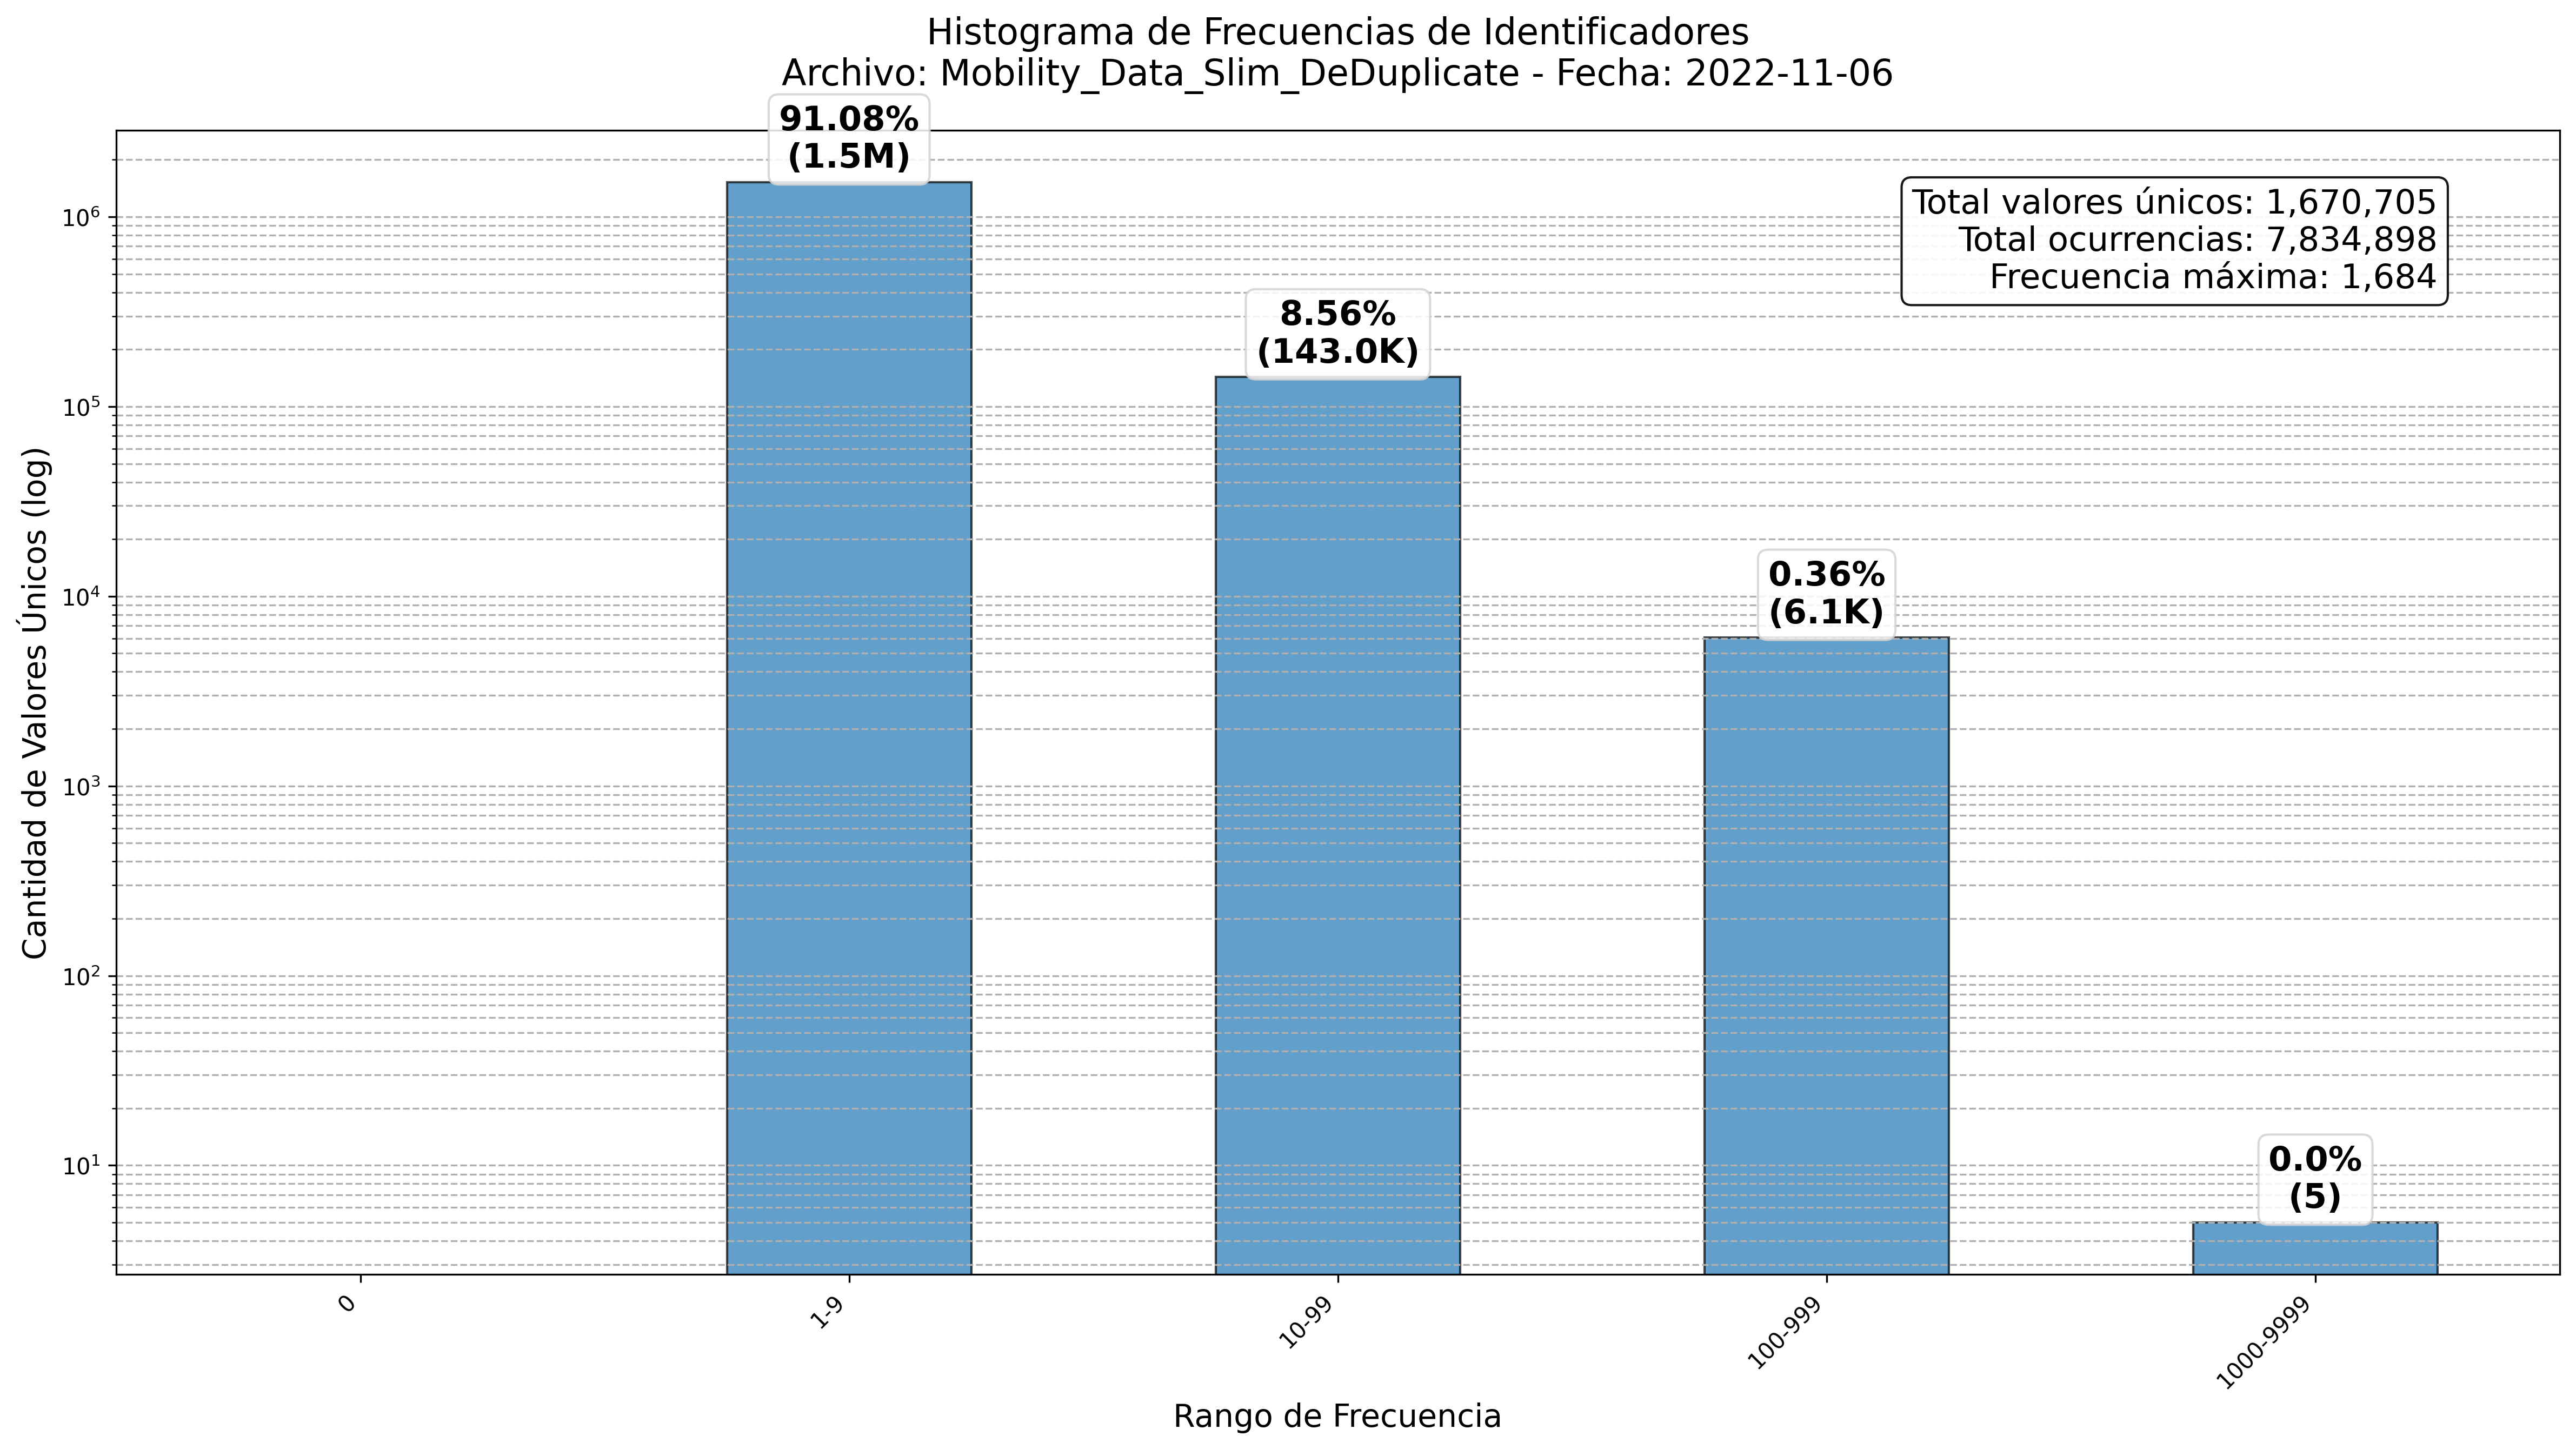
\includegraphics[width=\linewidth]{img/daily_histograms/histograma_identifier_Mobility_Data_Slim_DeDuplicate_2022-11-06.png}
        \caption{Histograma del 06/Nov/2022}
        \label{fig:sub1}
    \end{subfigure}
    \hfill
    \begin{subfigure}[t]{0.48\textwidth-1em}
        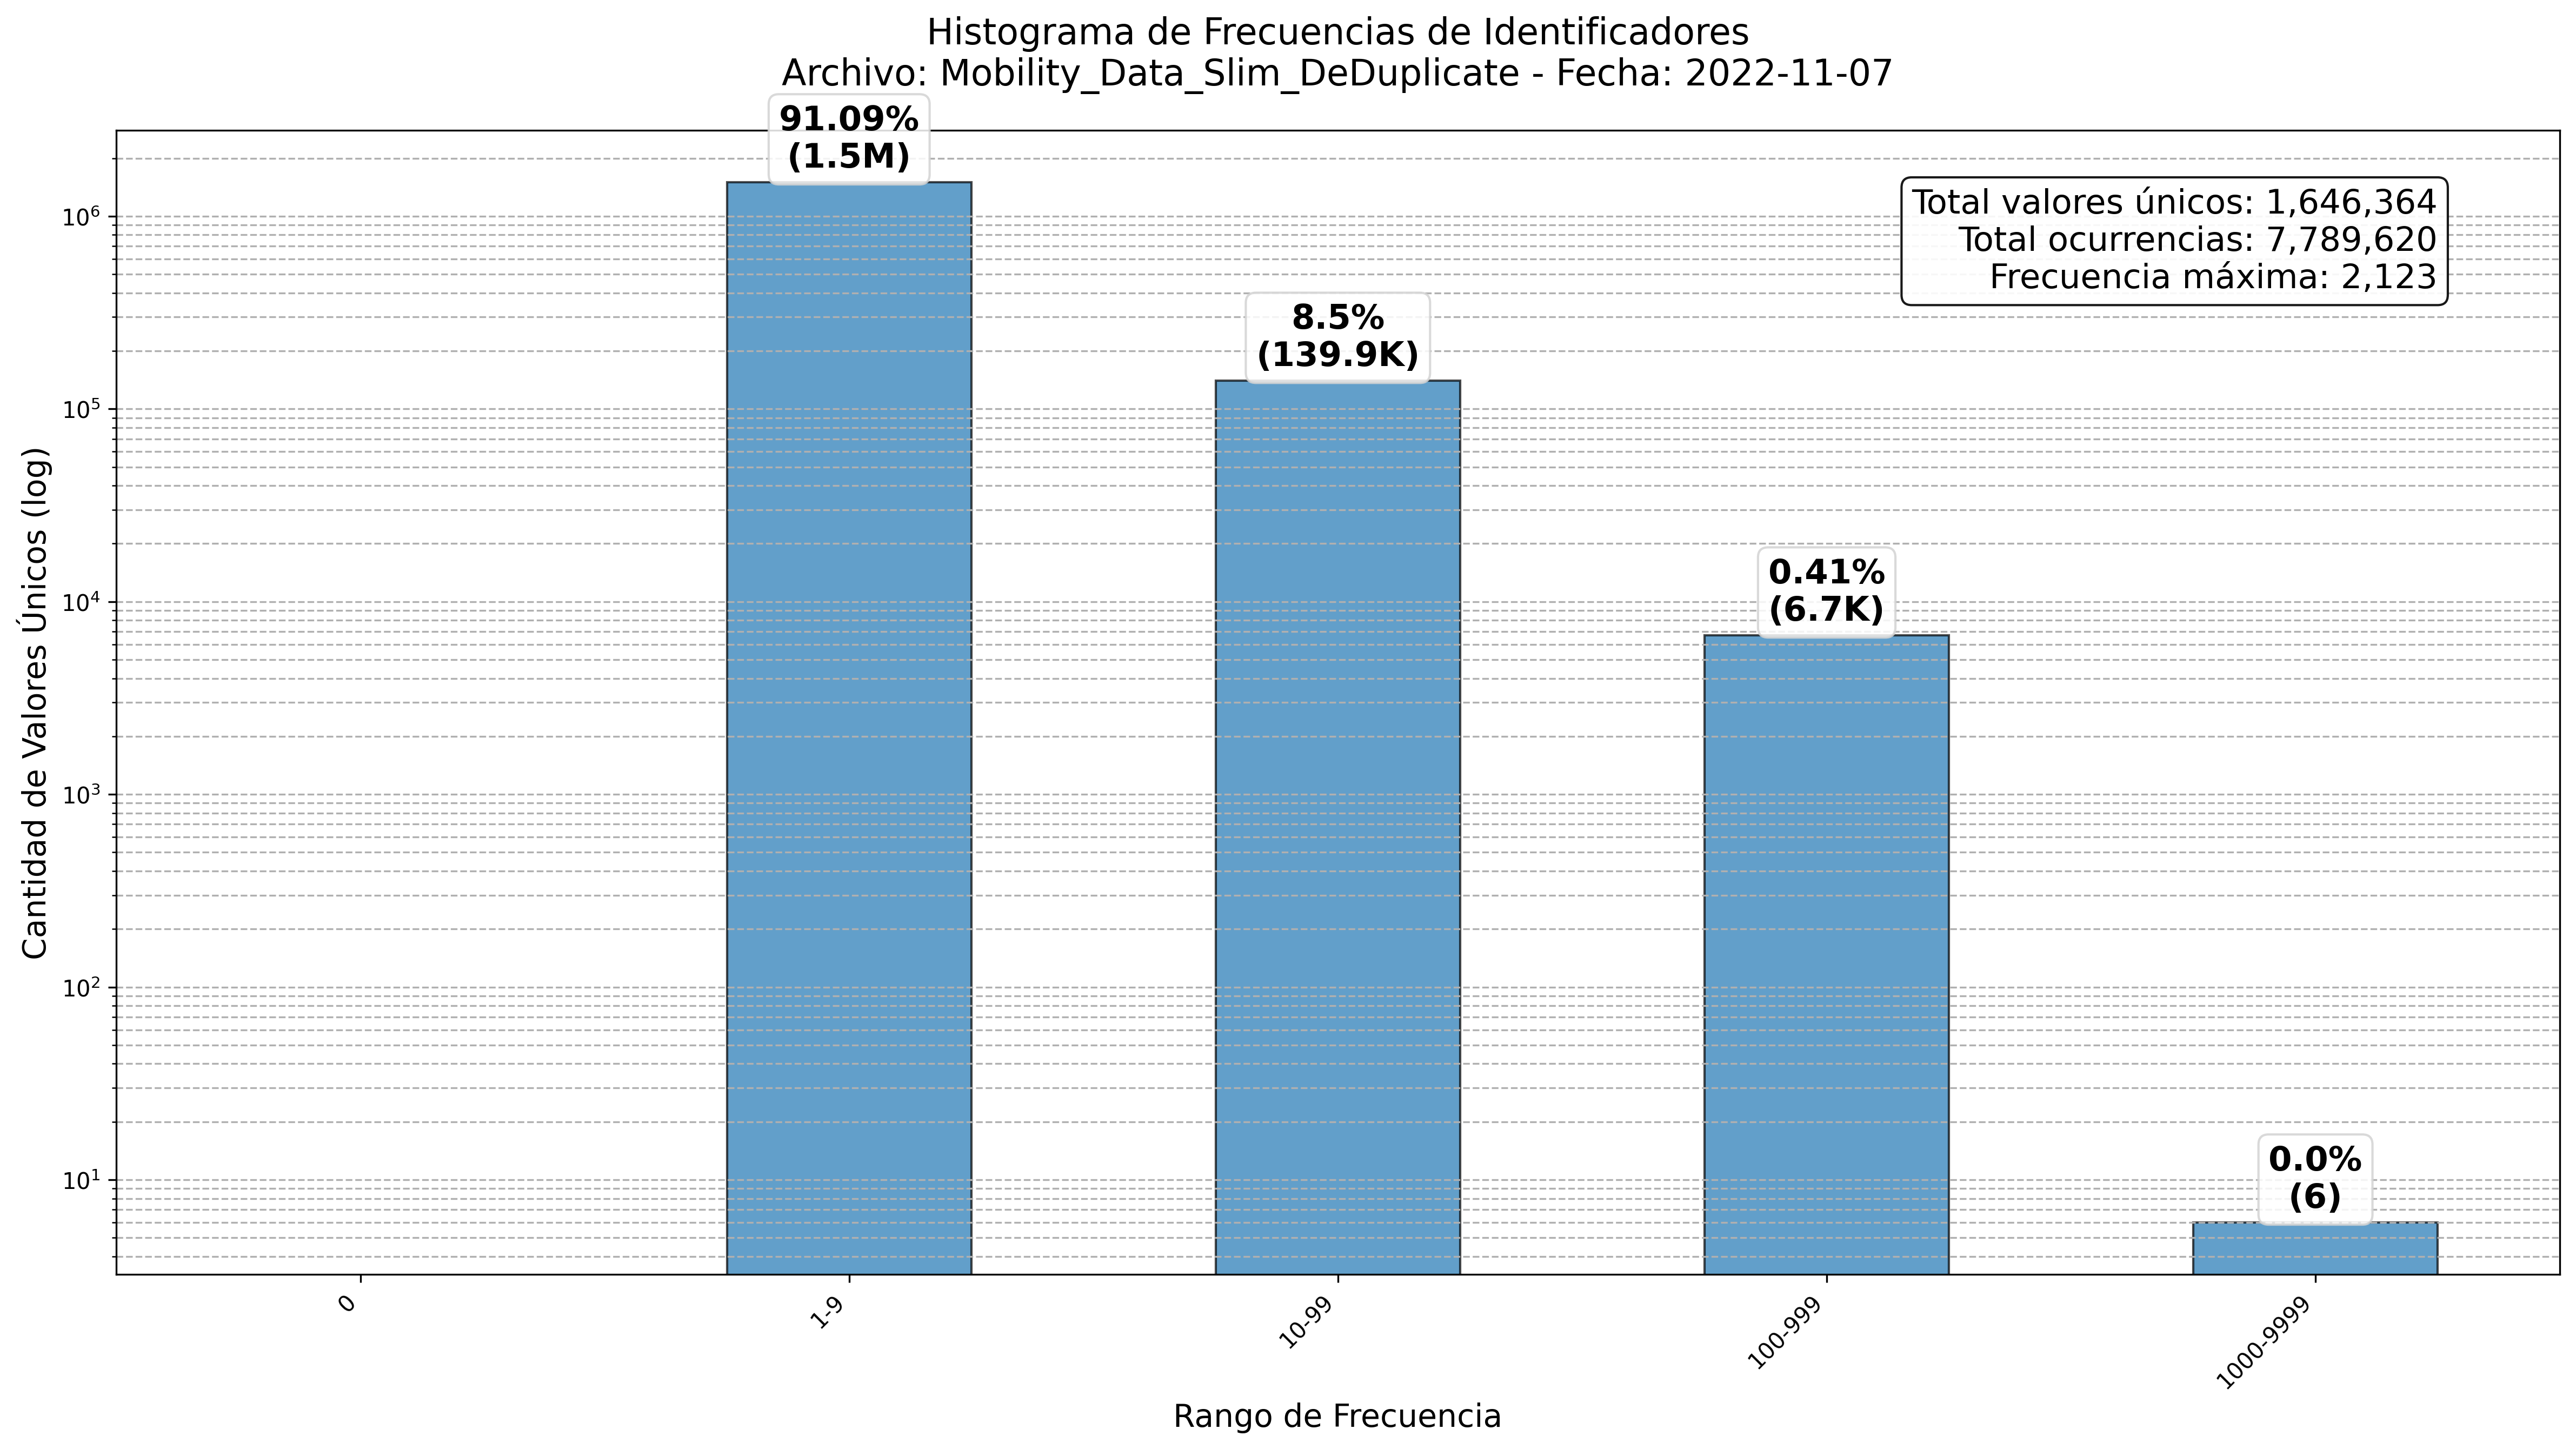
\includegraphics[width=\linewidth]{img/daily_histograms/histograma_identifier_Mobility_Data_Slim_DeDuplicate_2022-11-07.png}
        \caption{Histograma del 07/Nov/2022}
        \label{fig:sub2}
    \end{subfigure}

    \vspace{0.5cm}

    \begin{subfigure}[t]{0.48\textwidth-1em}
        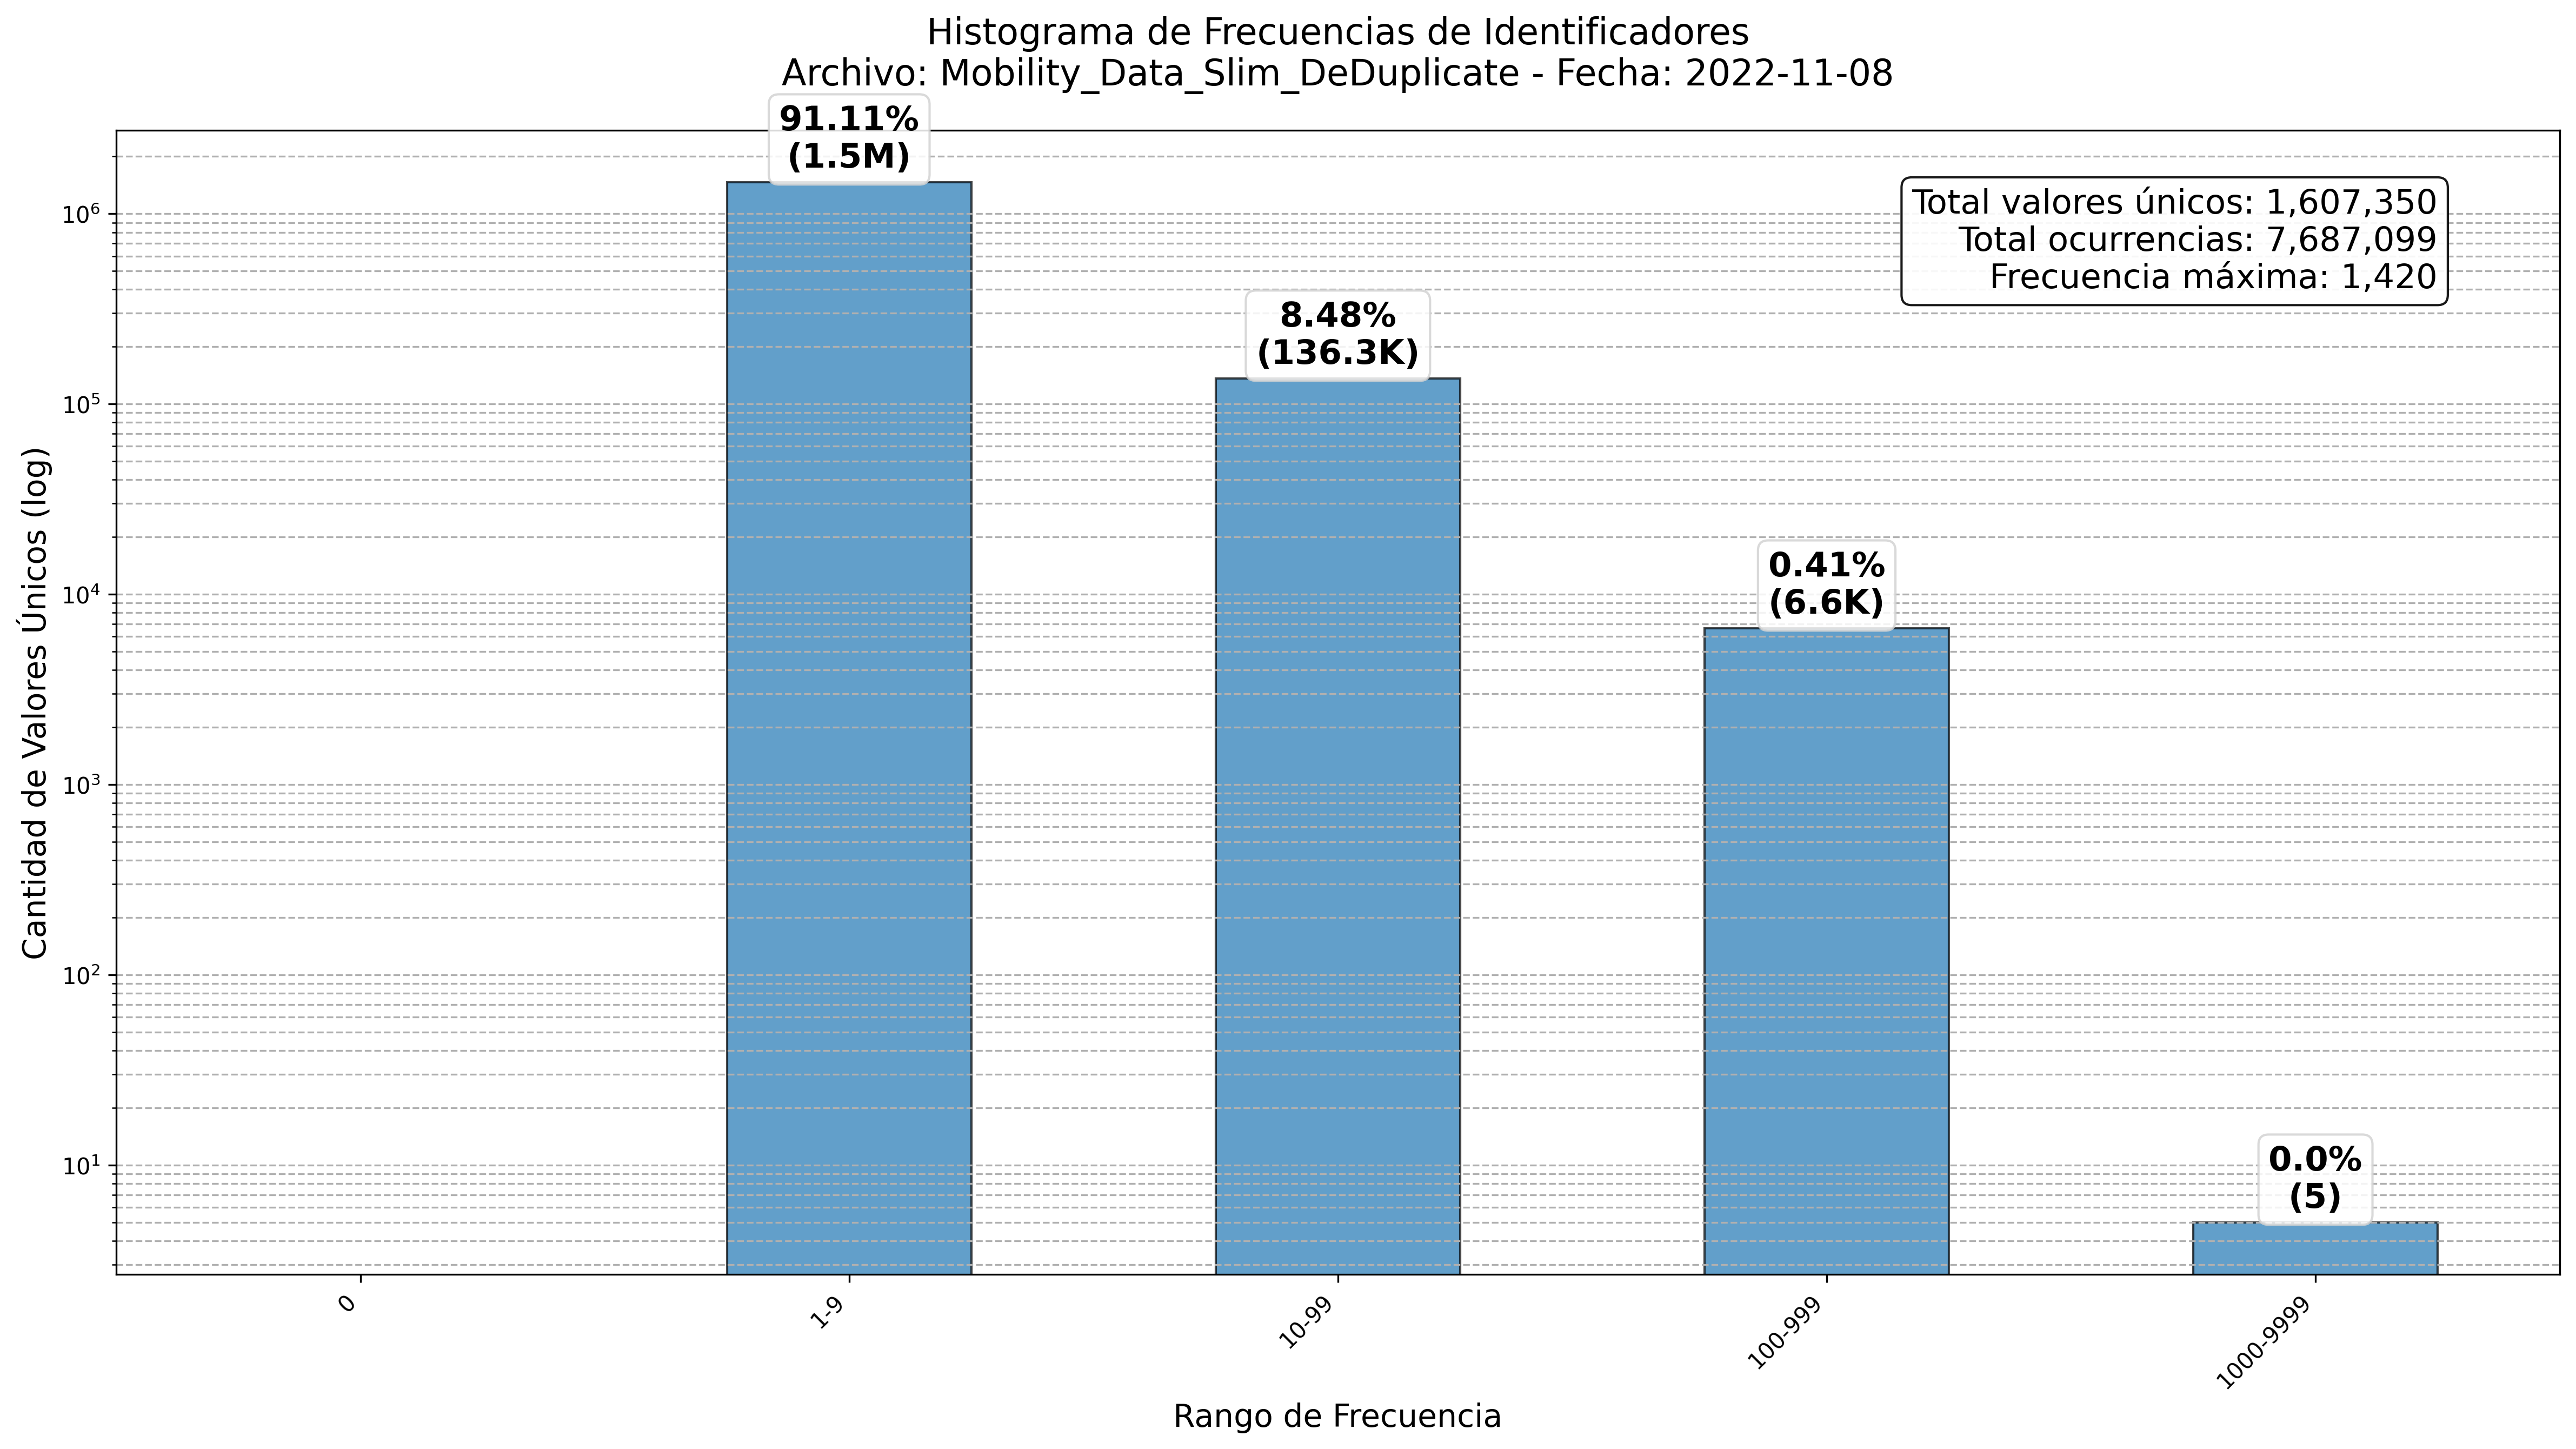
\includegraphics[width=\linewidth]{img/daily_histograms/histograma_identifier_Mobility_Data_Slim_DeDuplicate_2022-11-08.png}
        \caption{Histograma del 08/Nov/2022}
        \label{fig:sub3}
    \end{subfigure}
    \hfill
    \begin{subfigure}[t]{0.48\textwidth-1em}
        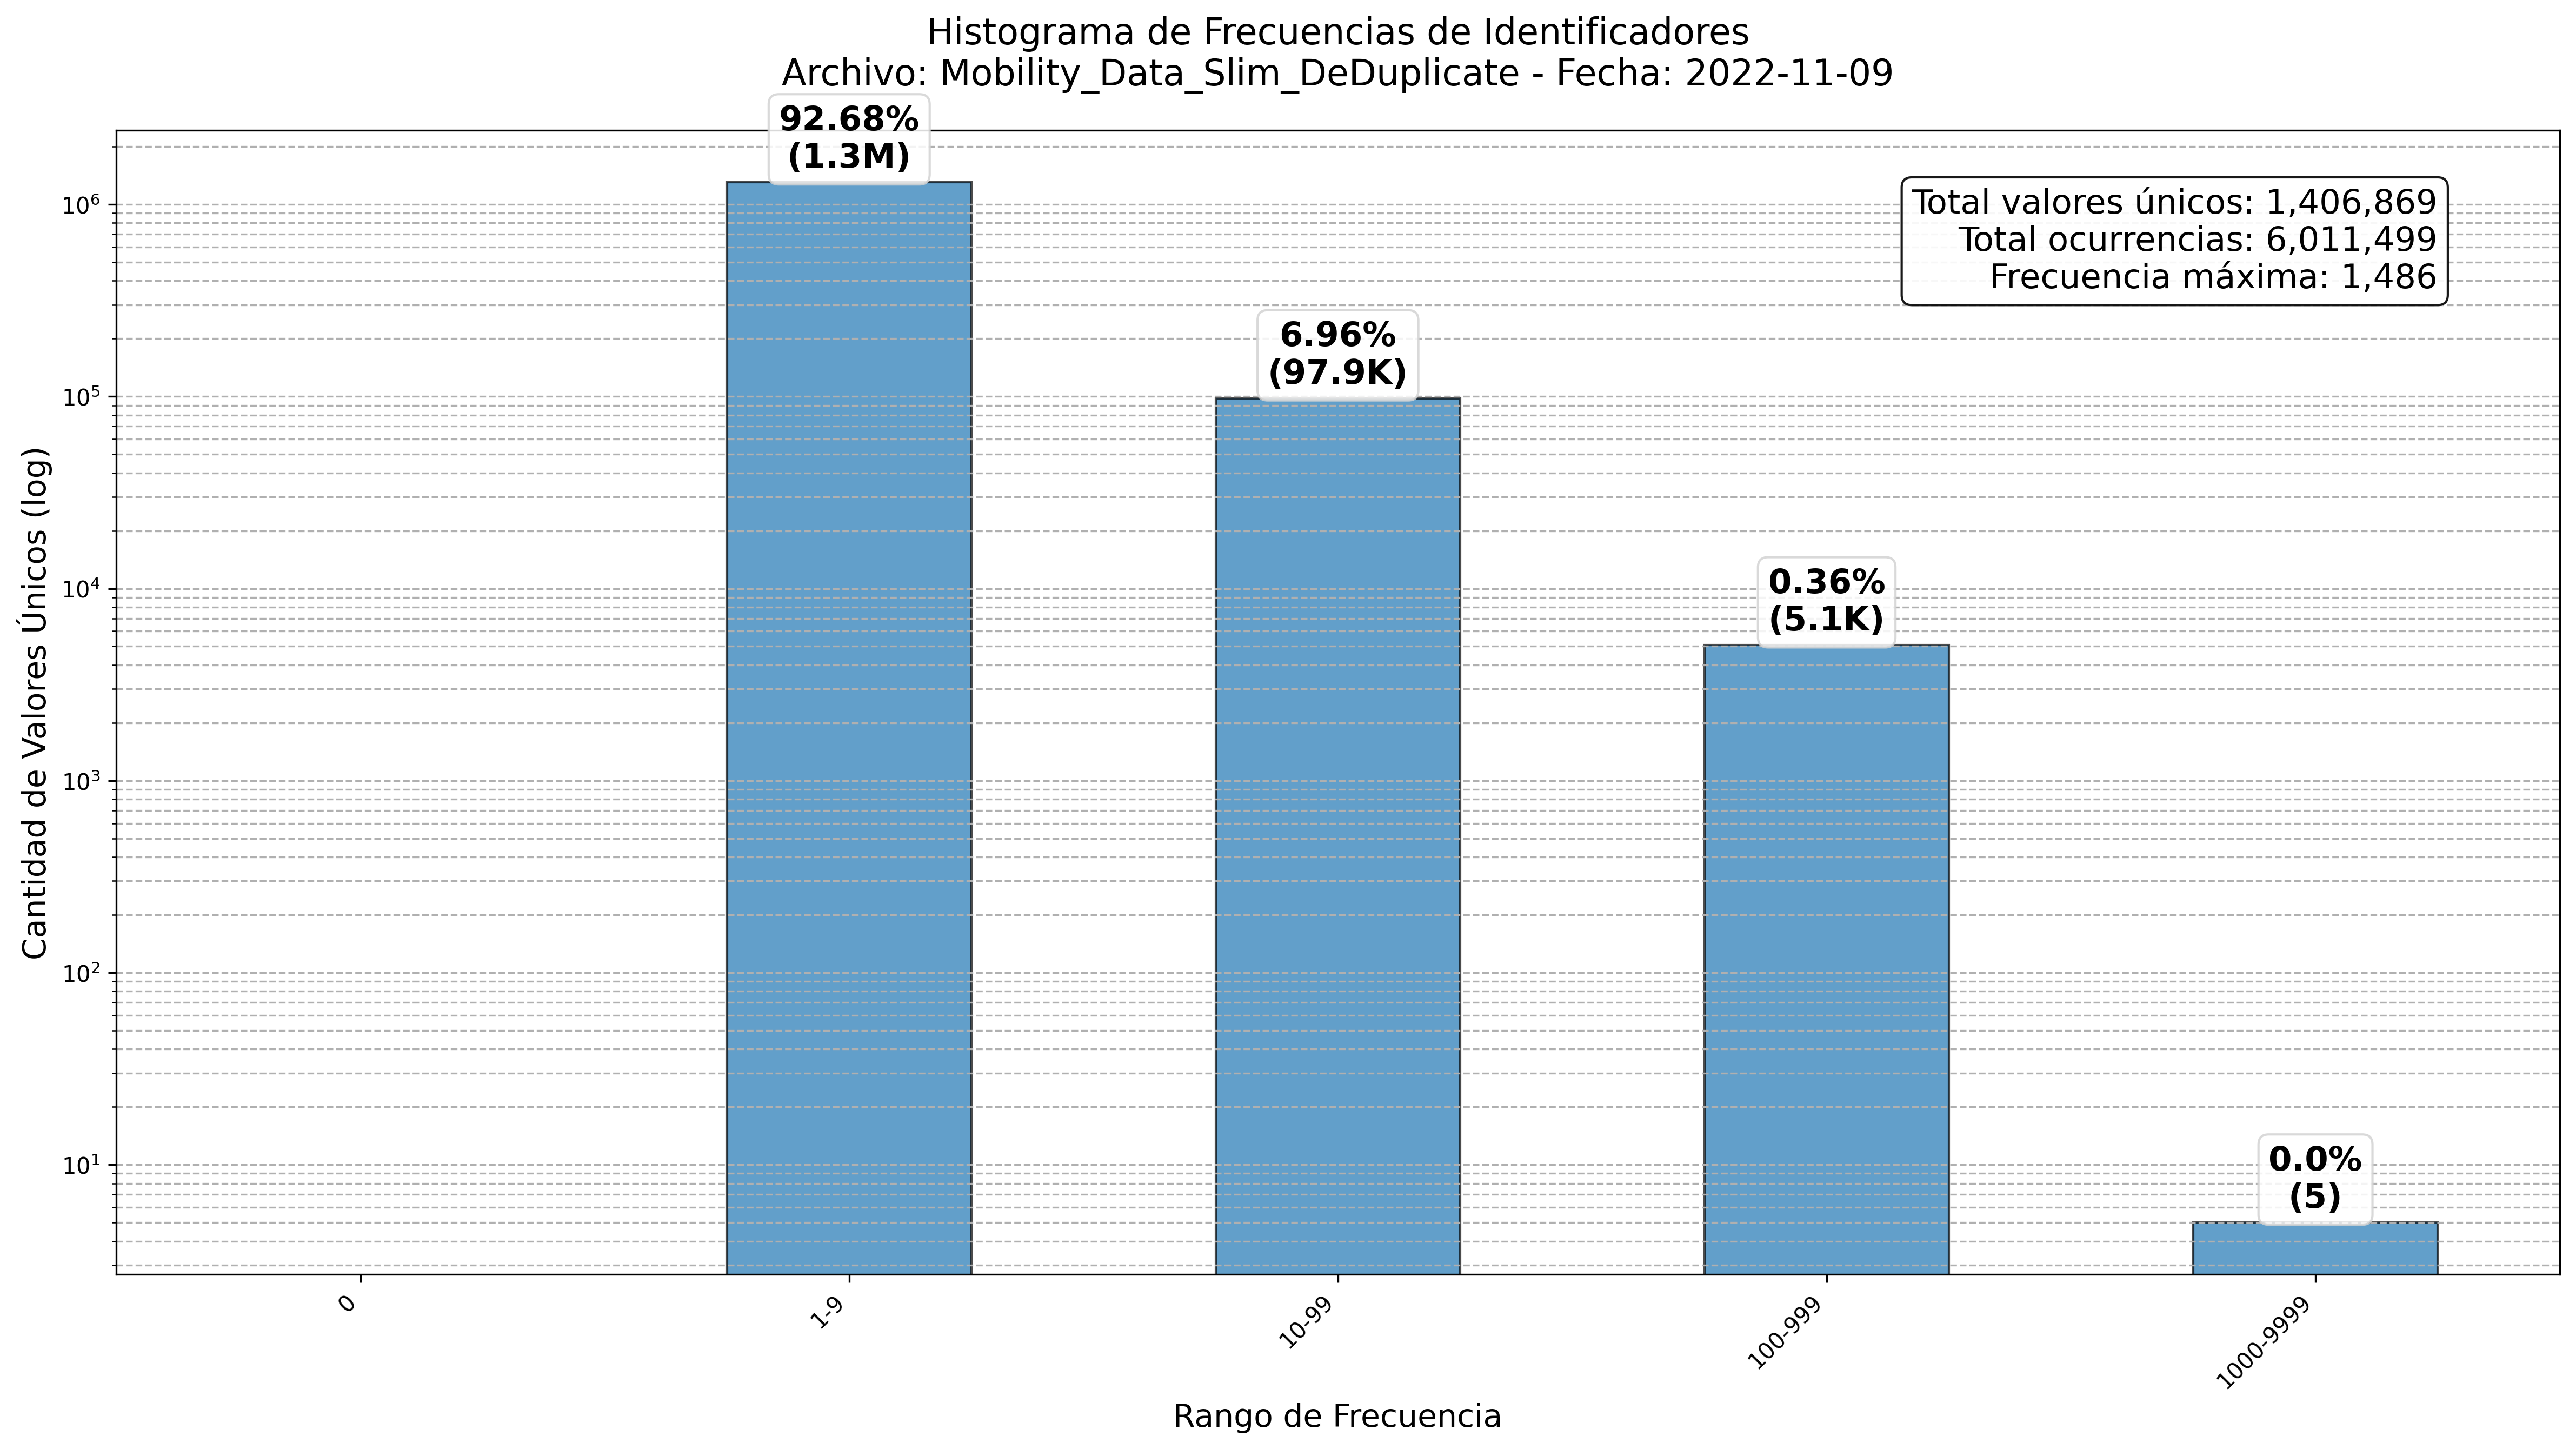
\includegraphics[width=\linewidth]{img/daily_histograms/histograma_identifier_Mobility_Data_Slim_DeDuplicate_2022-11-09.png}
        \caption{Histograma del 09/Nov/2022}
        \label{fig:sub4}
    \end{subfigure}
\end{figure}

\begin{figure}[H]
    \ContinuedFloat
    \centering
    \begin{subfigure}[t]{0.48\textwidth-1em}
        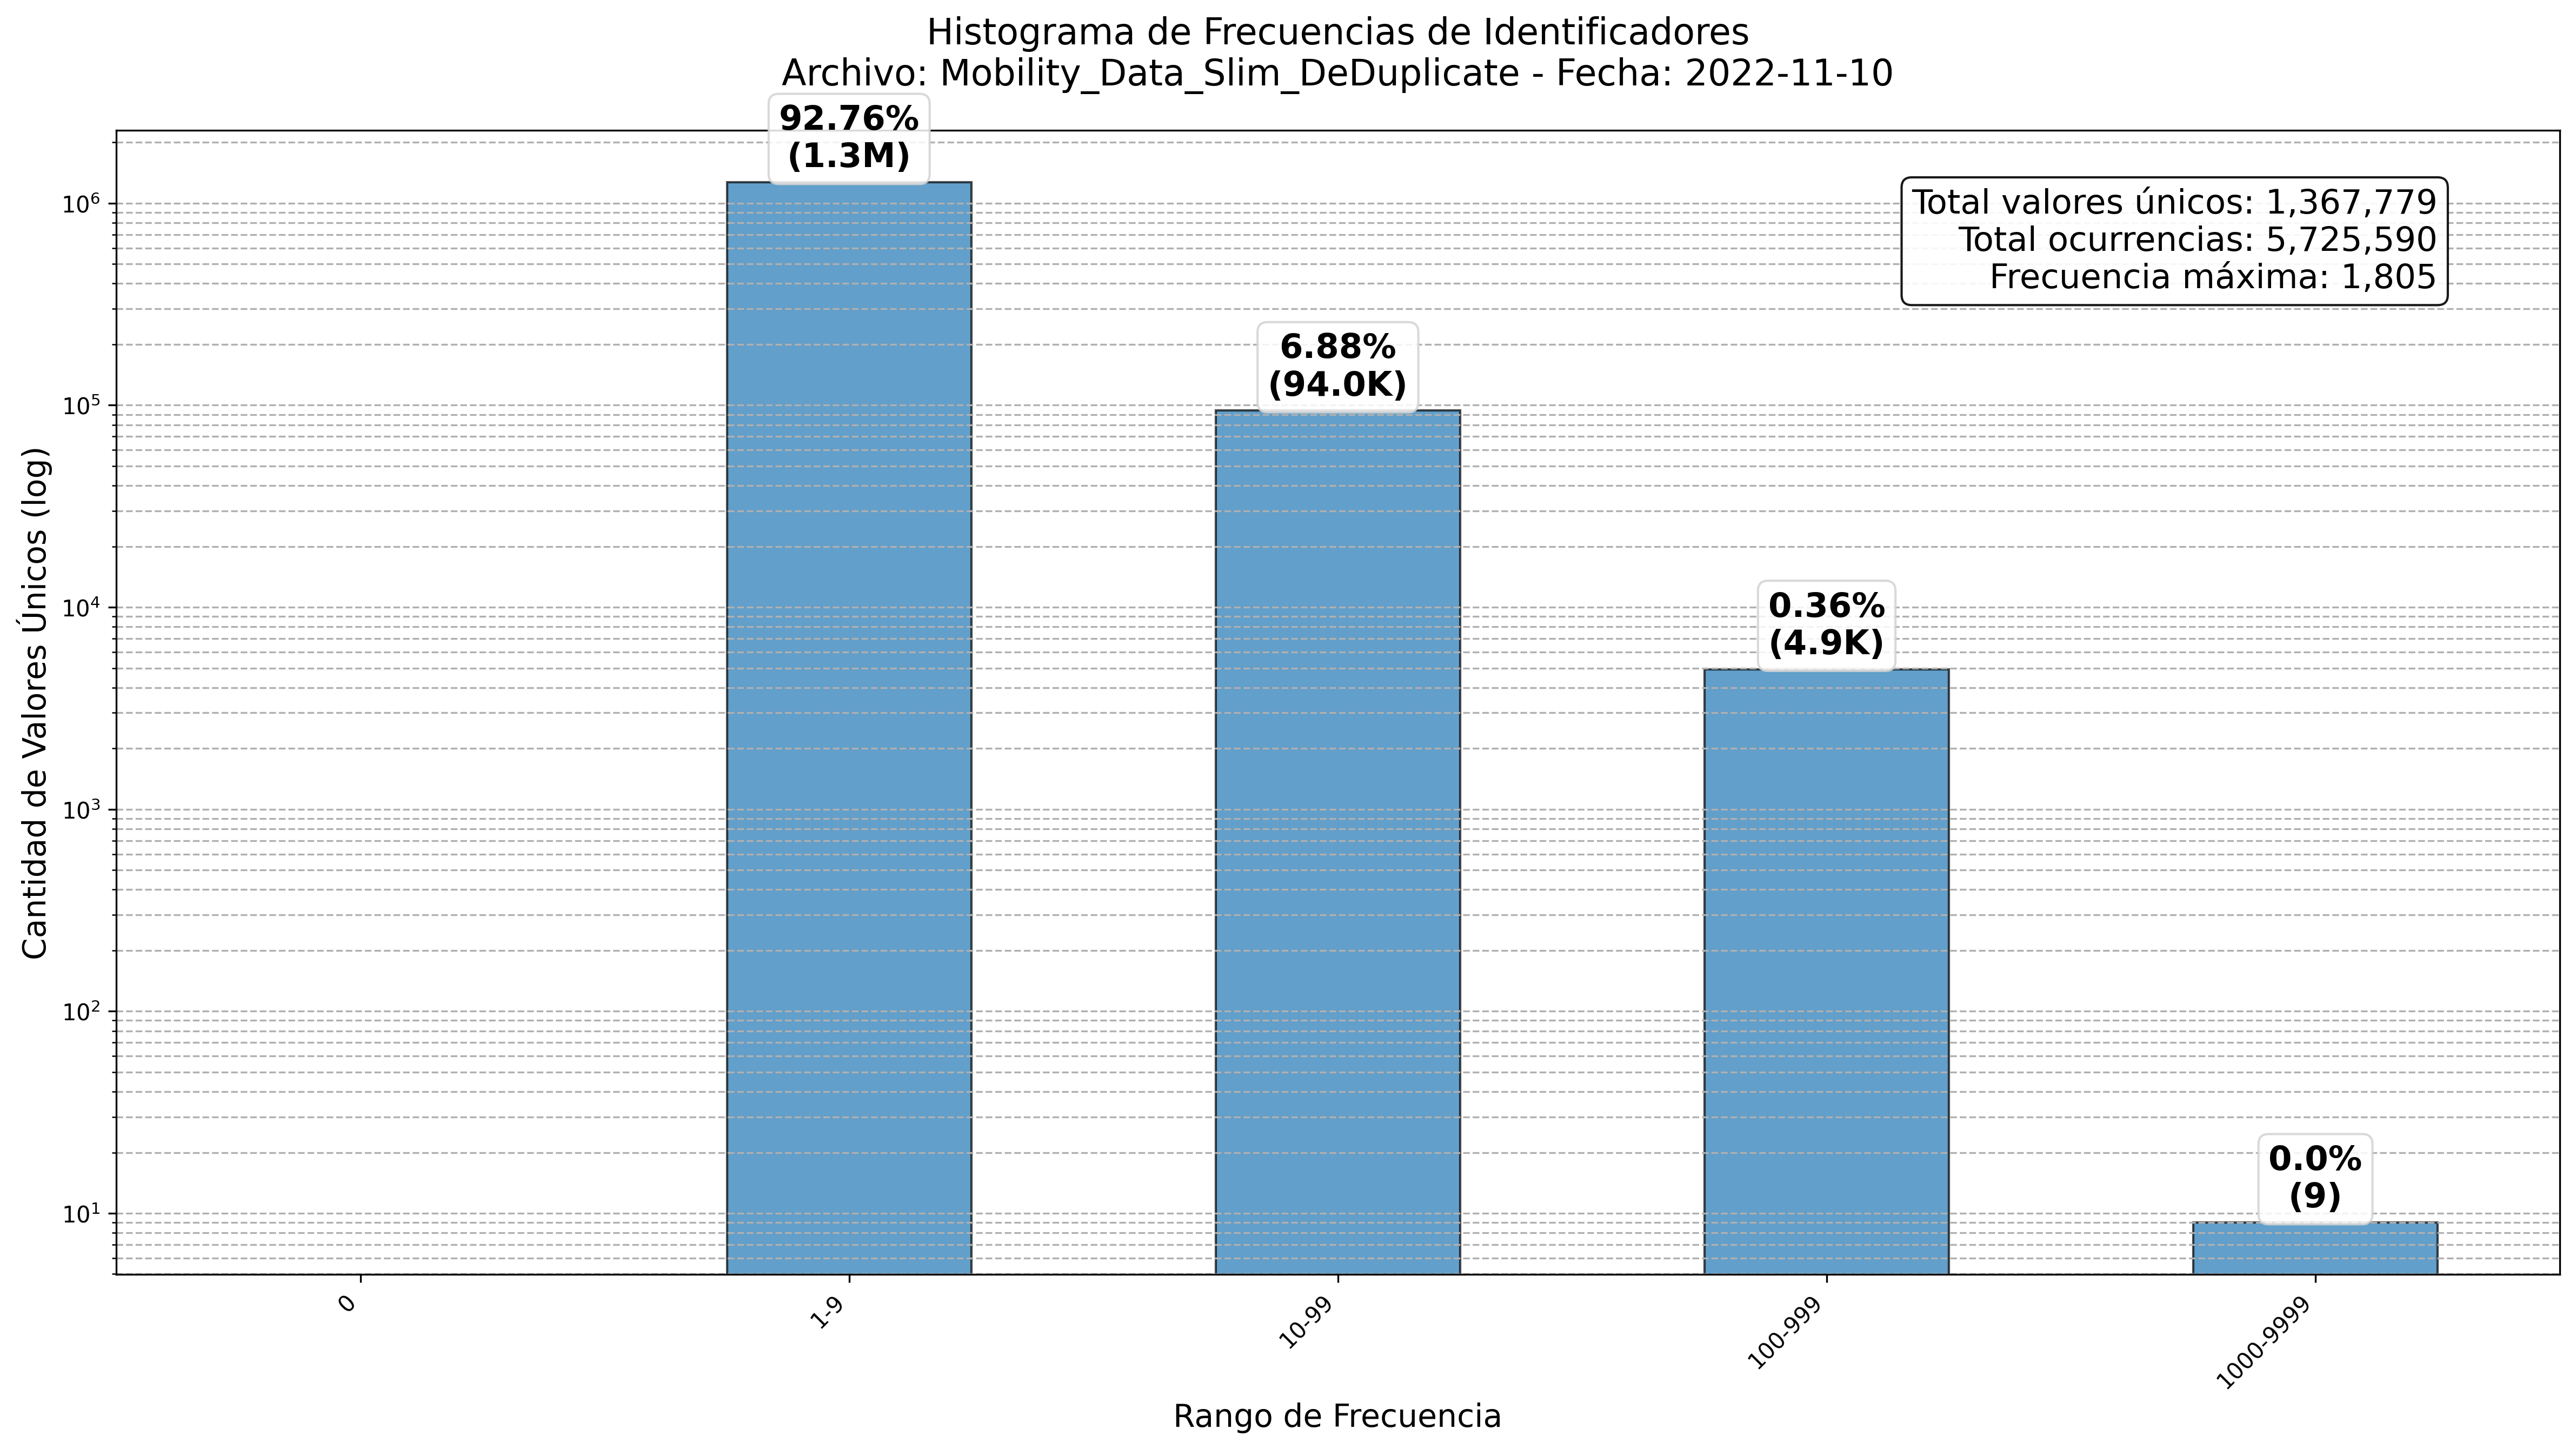
\includegraphics[width=\linewidth]{img/daily_histograms/histograma_identifier_Mobility_Data_Slim_DeDuplicate_2022-11-10.png}
        \caption{Histograma del 10/Nov/2022}
        \label{fig:sub5}
    \end{subfigure}
    \hfill
    \begin{subfigure}[t]{0.48\textwidth-1em}
        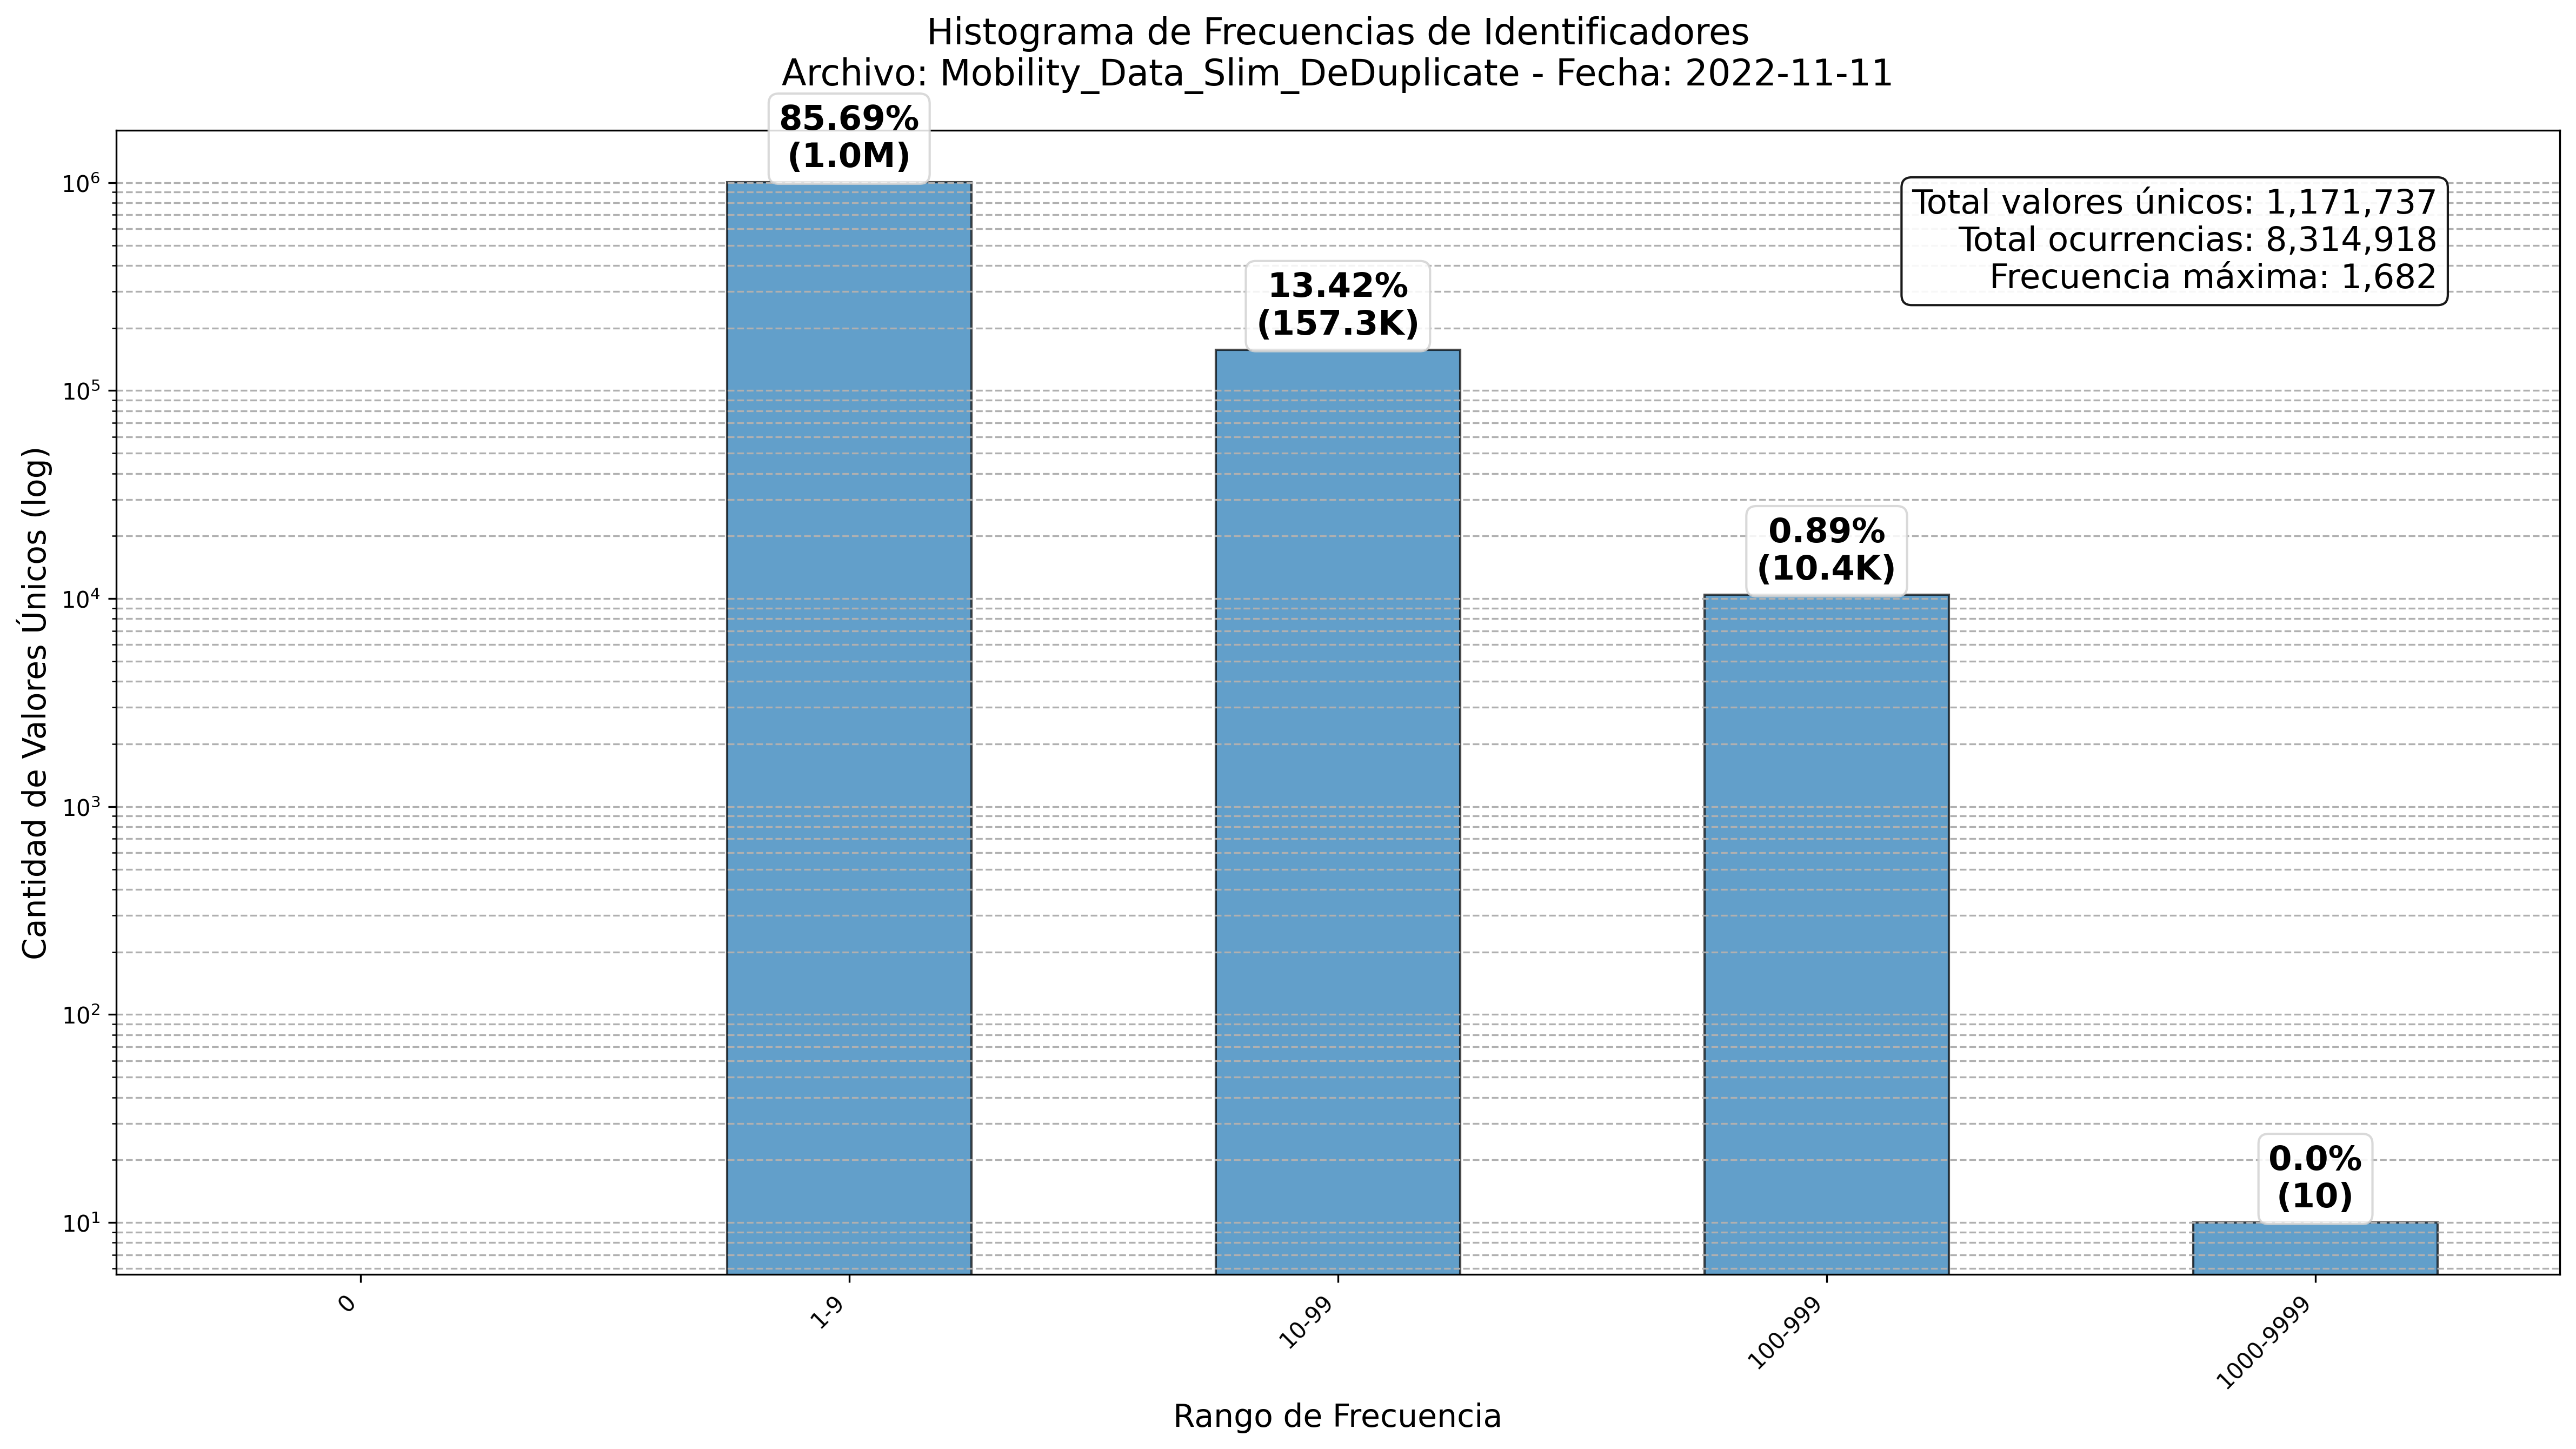
\includegraphics[width=\linewidth]{img/daily_histograms/histograma_identifier_Mobility_Data_Slim_DeDuplicate_2022-11-11.png}
        \caption{Histograma del 11/Nov/2022}
        \label{fig:sub6}
    \end{subfigure}

    \vspace{0.5cm}

    \begin{subfigure}[t]{0.48\textwidth-1em}
        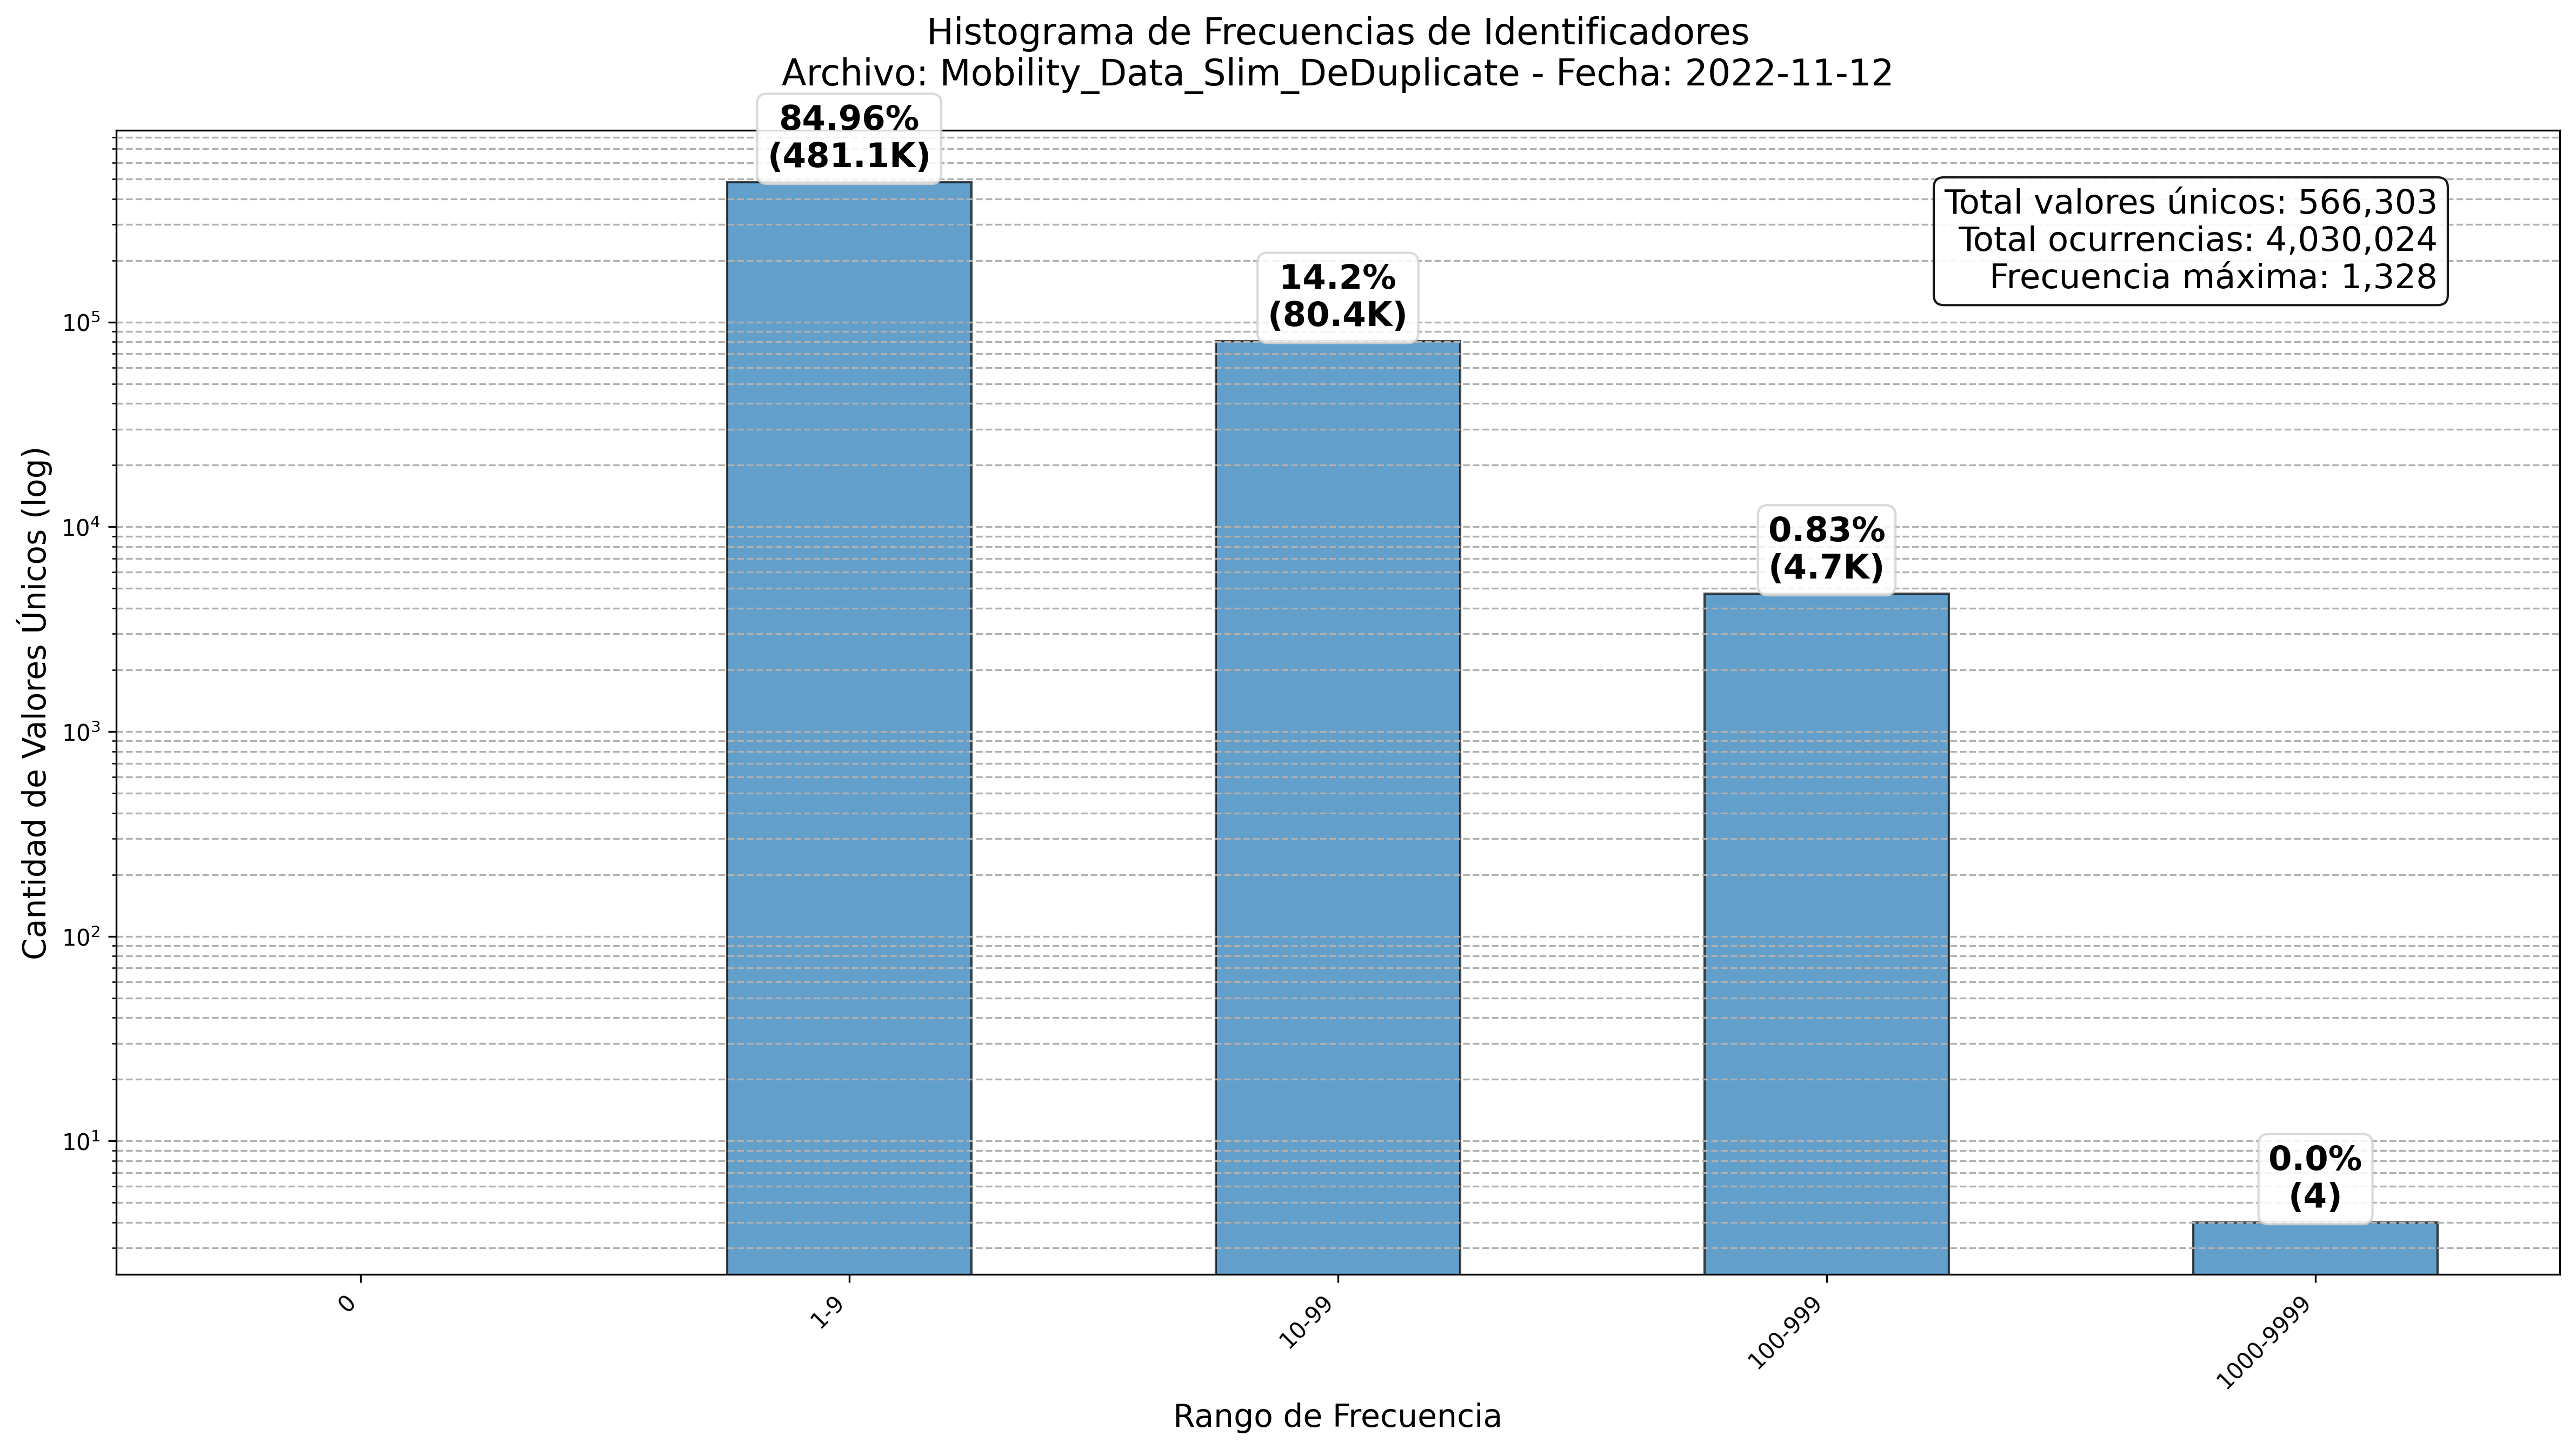
\includegraphics[width=\linewidth]{img/daily_histograms/histograma_identifier_Mobility_Data_Slim_DeDuplicate_2022-11-12.png}
        \caption{Histograma del 12/Nov/2022}
        \label{fig:sub7}
    \end{subfigure}
    \hfill
    \begin{subfigure}[t]{0.48\textwidth-1em}
        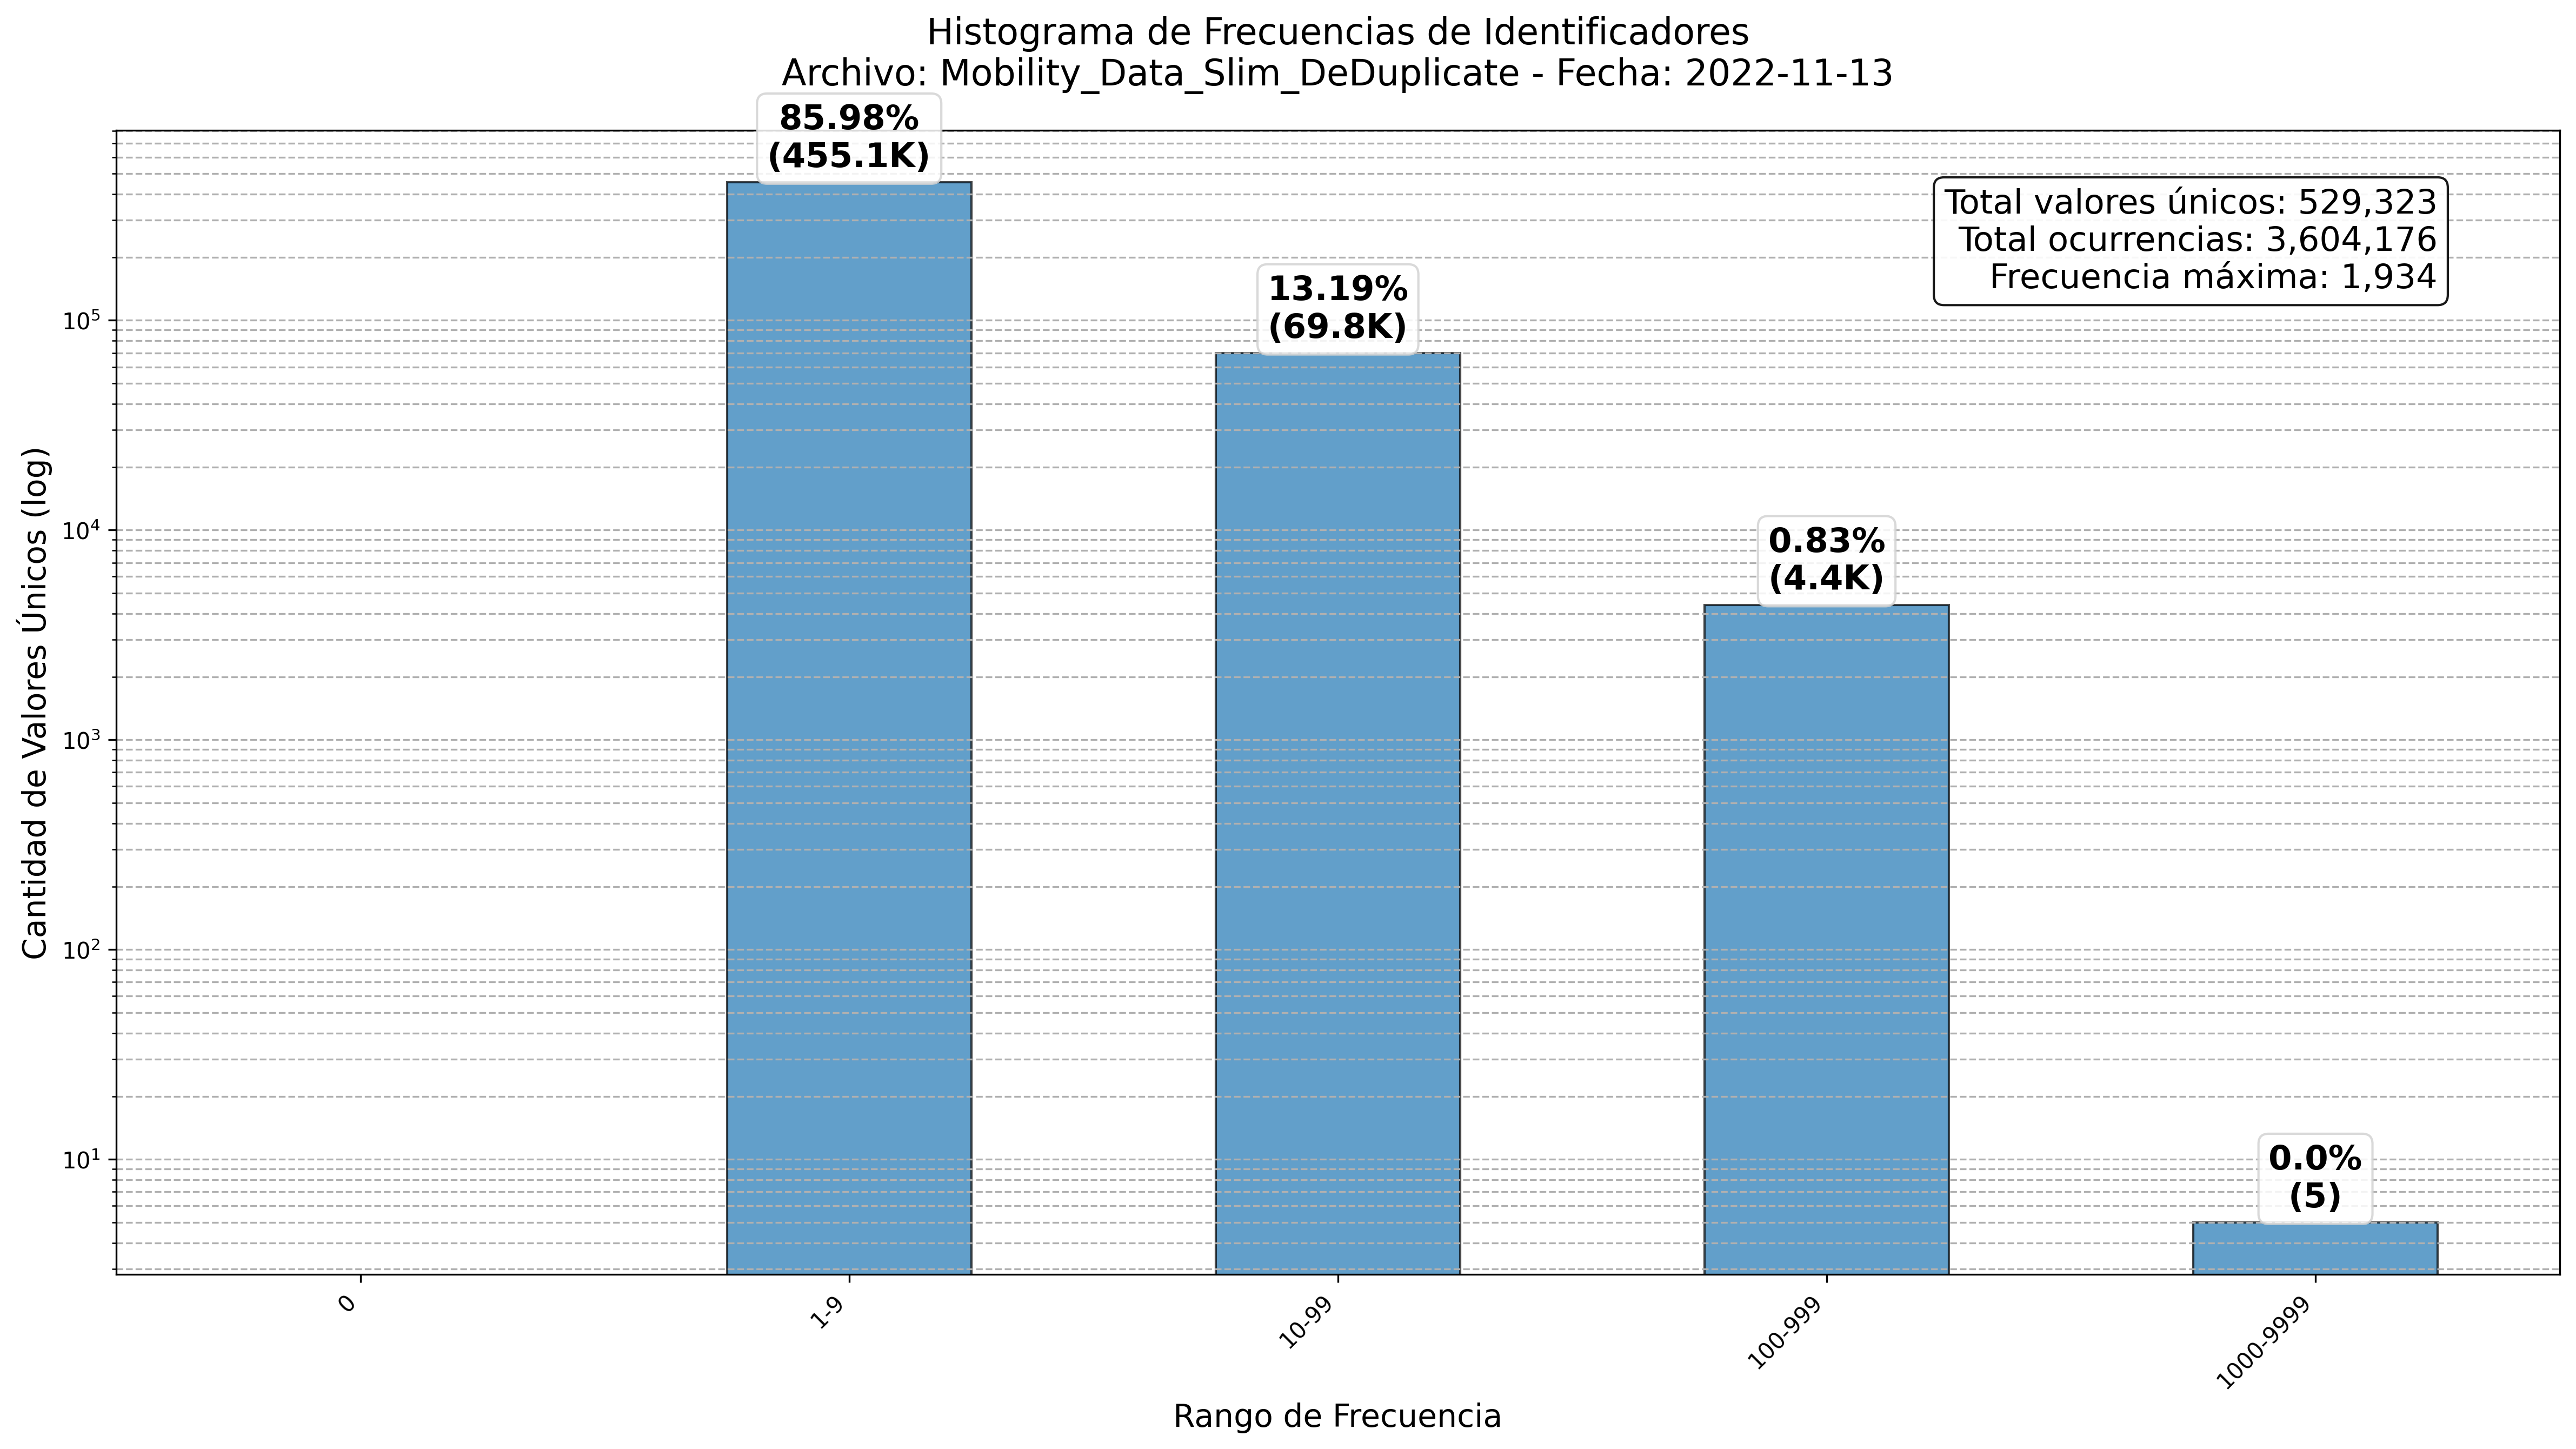
\includegraphics[width=\linewidth]{img/daily_histograms/histograma_identifier_Mobility_Data_Slim_DeDuplicate_2022-11-13.png}
        \caption{Histograma del 13/Nov/2022}
        \label{fig:sub8}
    \end{subfigure}

    \vspace{0.5cm}

    \begin{subfigure}[t]{0.48\textwidth-1em}
        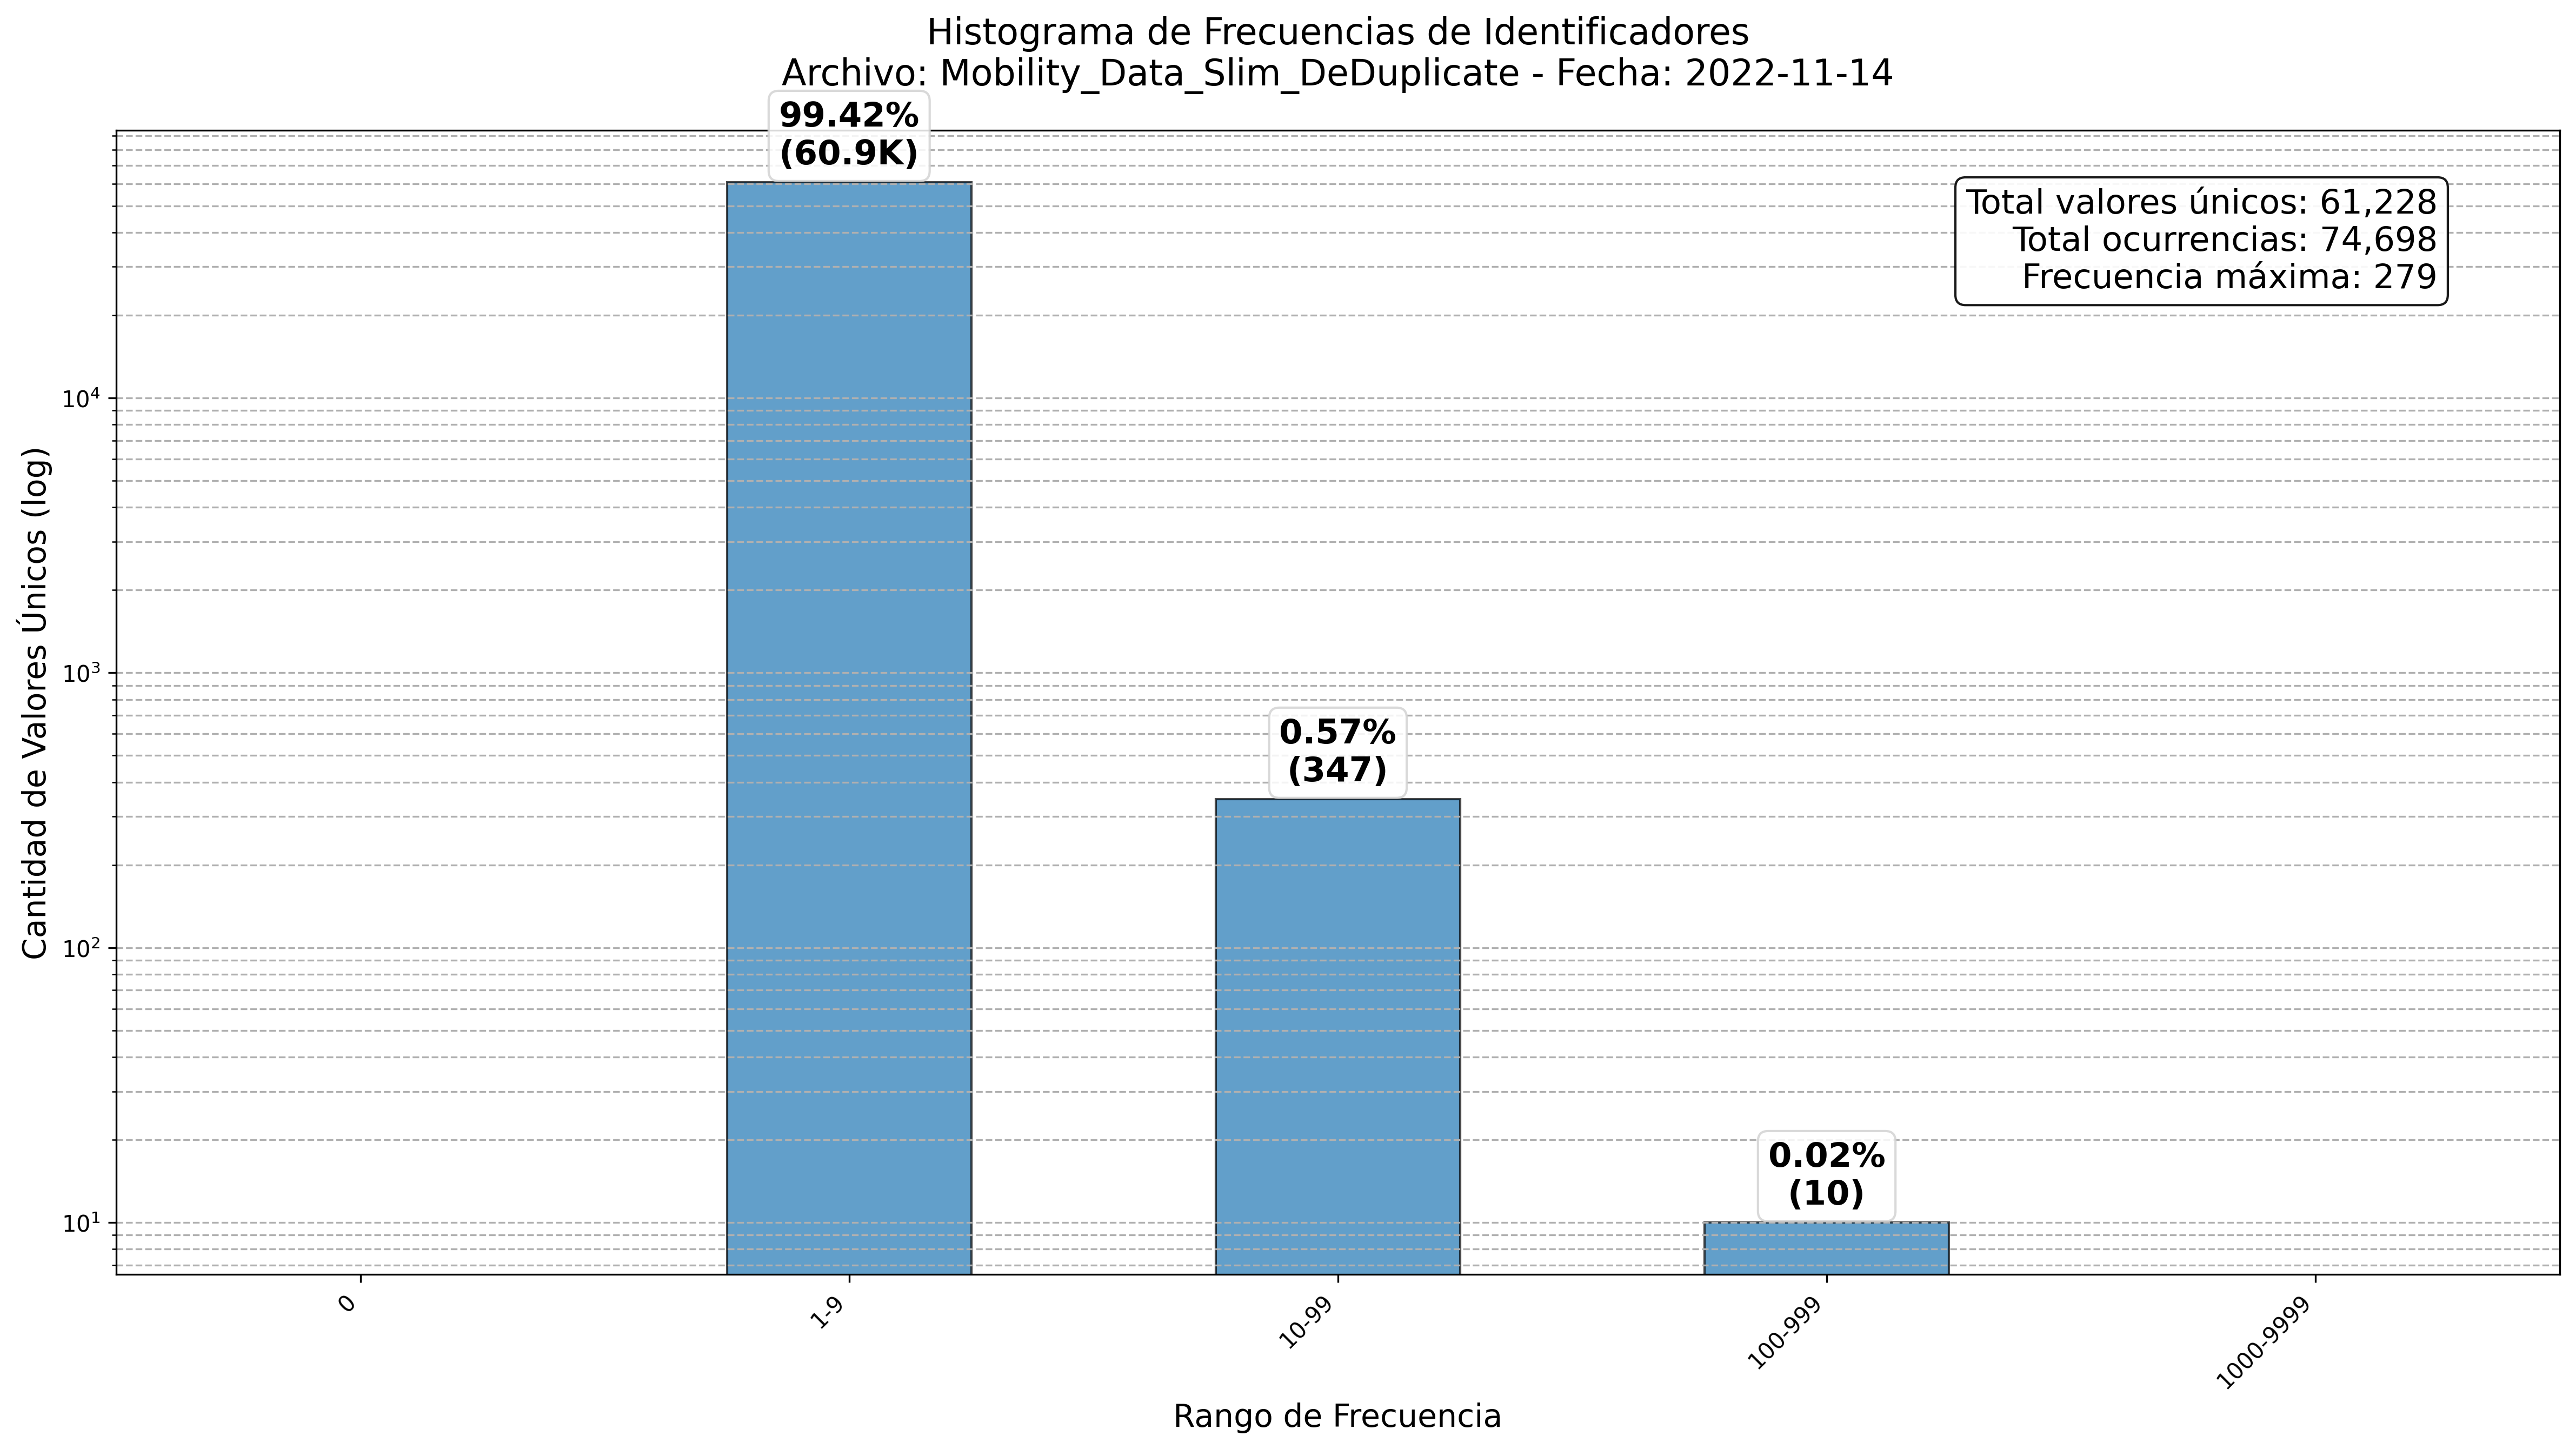
\includegraphics[width=\linewidth]{img/daily_histograms/histograma_identifier_Mobility_Data_Slim_DeDuplicate_2022-11-14.png}
        \caption{Histograma del 14/Nov/2022}
        \label{fig:sub9}
    \end{subfigure}
    \hfill
    \begin{subfigure}[t]{0.48\textwidth-1em}
        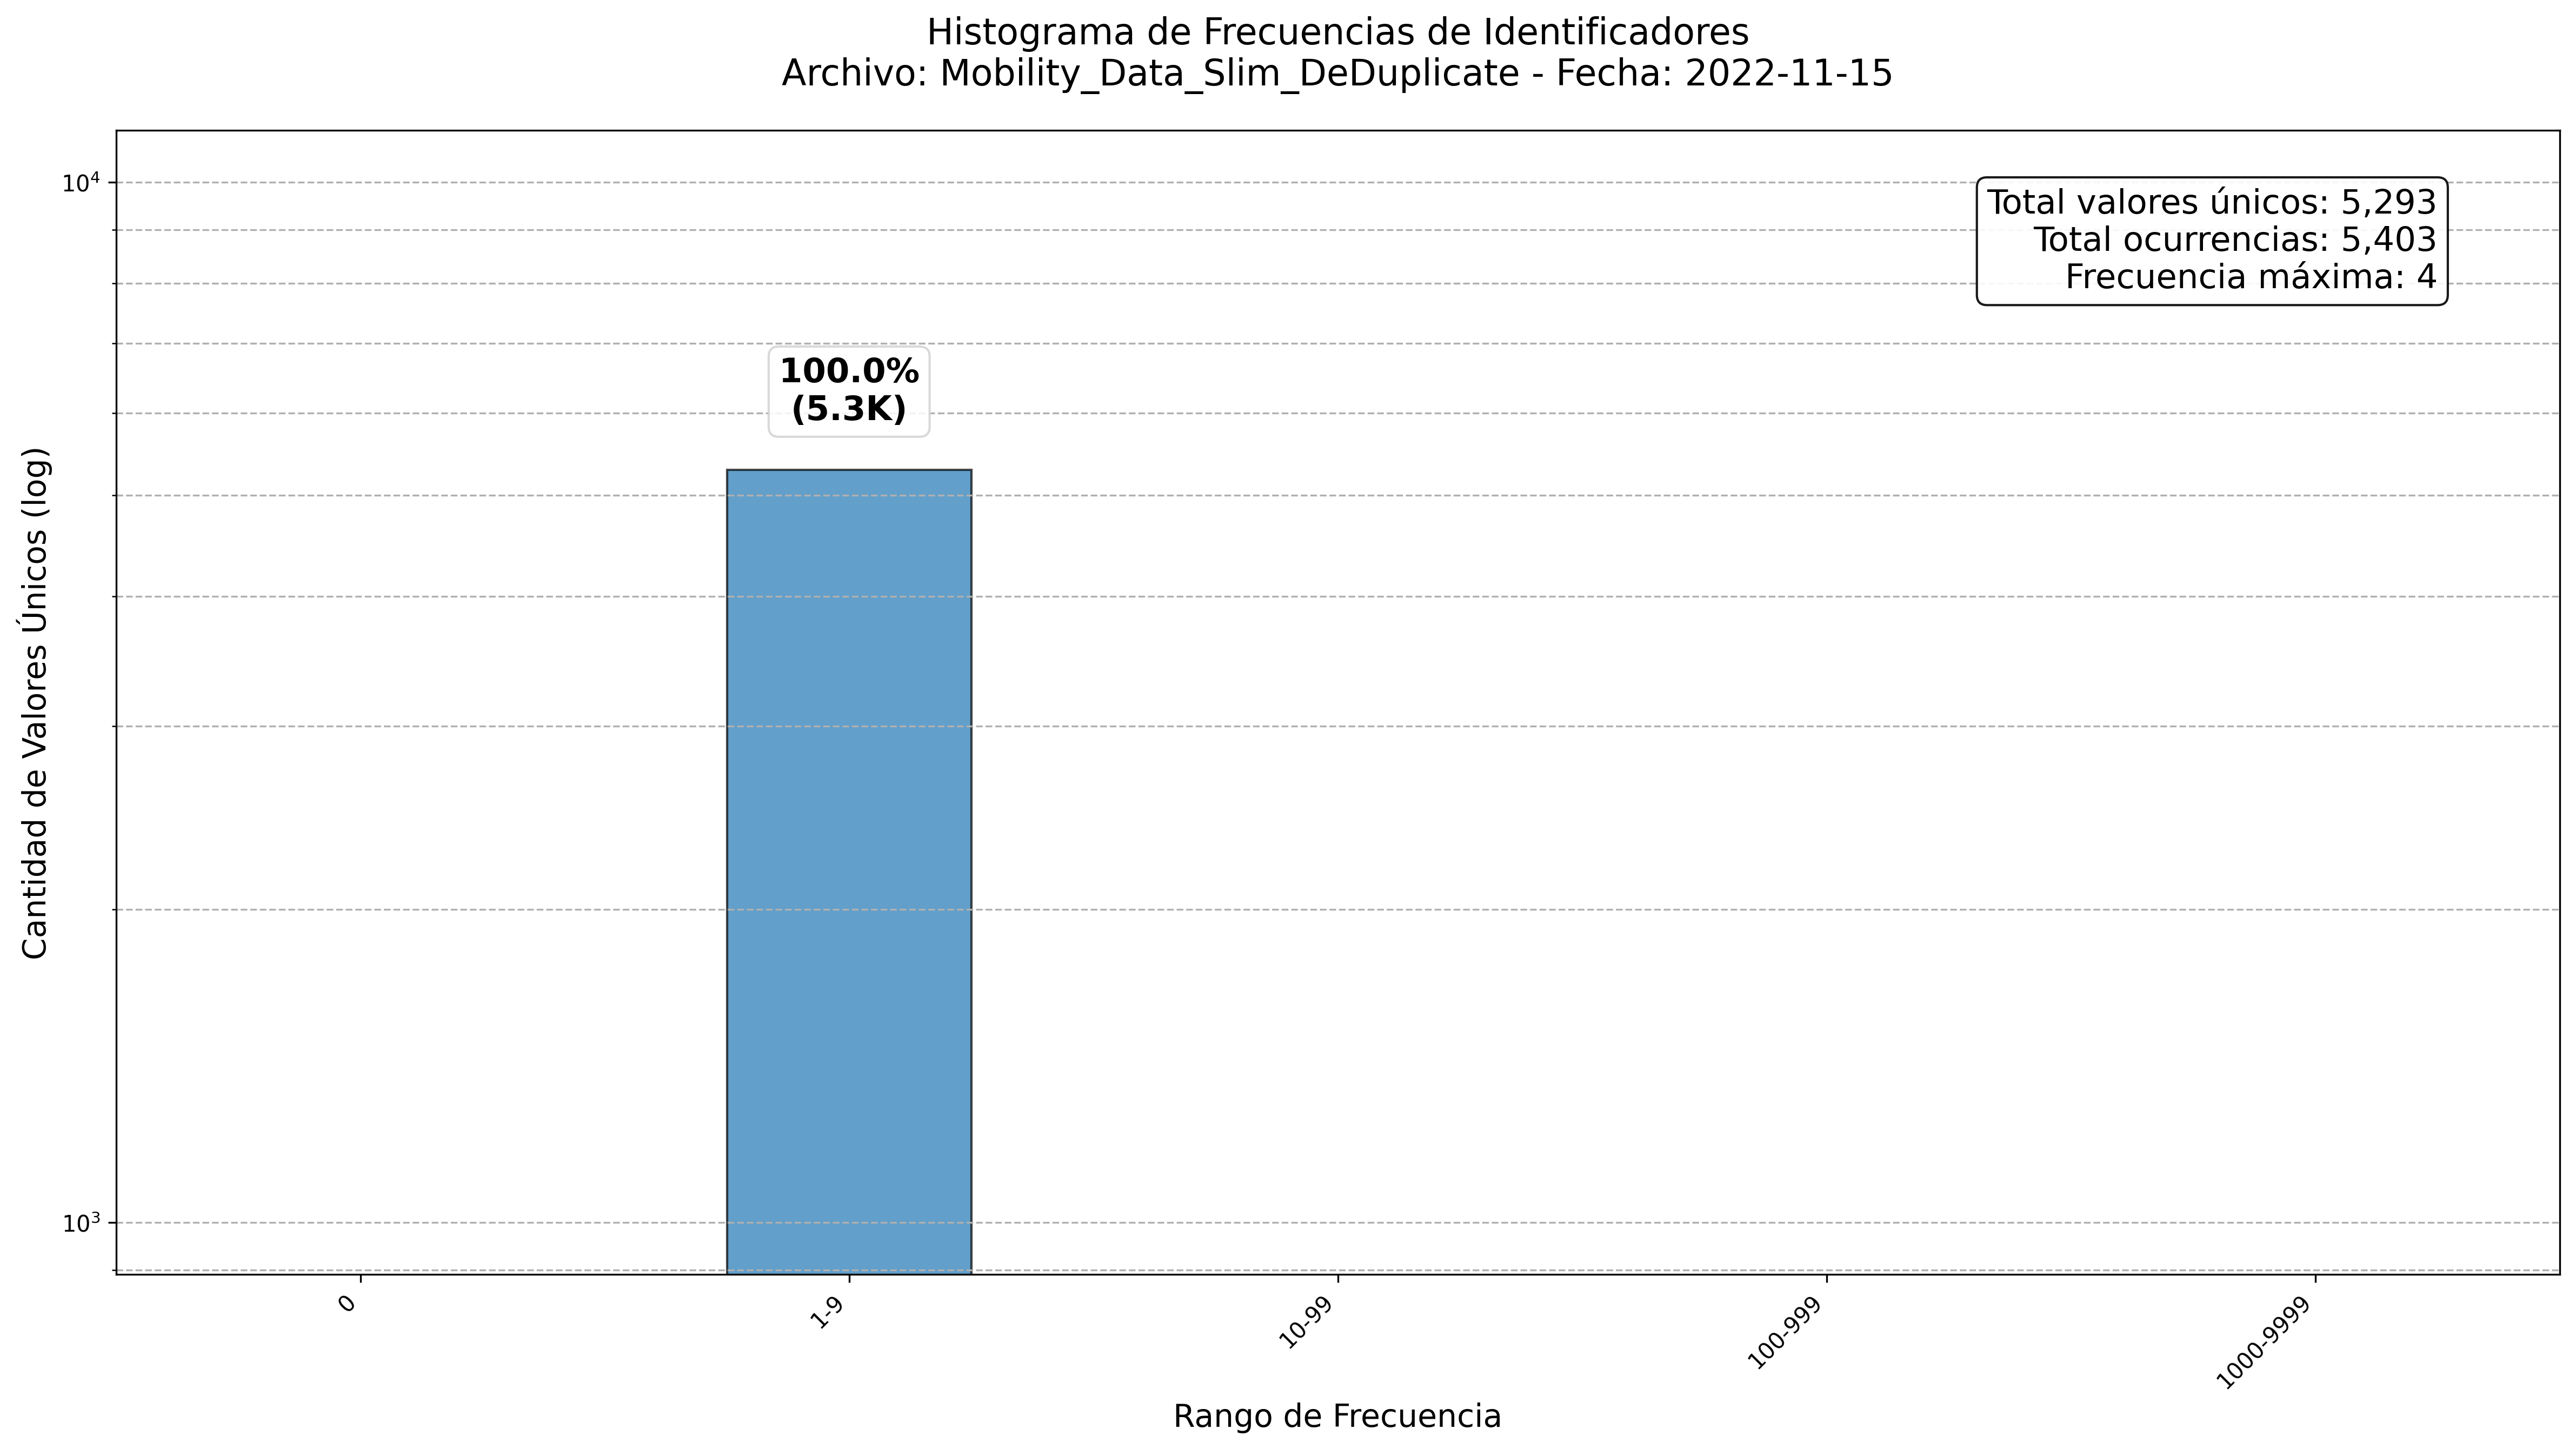
\includegraphics[width=\linewidth]{img/daily_histograms/histograma_identifier_Mobility_Data_Slim_DeDuplicate_2022-11-15.png}
        \caption{Histograma del 15/Nov/2022}
        \label{fig:sub10}
    \end{subfigure}
    \caption{Comparación de distribución de individuos por día.}
    \label{fig:histogramas_daily}
\end{figure}

De la figura anterior se puede observar que la distribución de individuos por día es bastante similar a la distribución vista en la Figura \ref{fig:identifier_histogram_deduplicate}, donde se observa que la mayoría de los individuos tienen una frecuncia de aparición baja. Además se puede ver que los primros seis días hay en promedio \textbf{1,400,000} de individuos, mientras que los últimos cuatro días este valor va disminuyendo hasta llegar a \textbf{5,293} individuos el día 15 de noviembre. Esto puede ser un indicativo de que la recolección de datos no fue constante a lo largo del tiempo, lo que podría deberse a diversos factores como problemas técnicos o cambios en el comportamiento de los individuos.

\chapter{Observaciones y recomendaciones}
% --------------------------
% Observaciones y recomendaciones
% --------------------------
Durante el proceso de caracterización de datos de trayectorias individuales del Capítulo \ref{sec:caracterizacion} se identificaron aspectos importantes que impactan la calidad del análisis y la validez de los resultados obtenidos. Esta sección presenta las principales observaciones derivadas del proceso y las recomendaciones para mejorar futuros análisis.

\section{Calidad de datos}
La caracterizacíón reveló que el \textbf{68.73\%} de los registros tienen una precisión GPS dentro del rango satelital (1-20 metros), mientras que el \textbf{31.27\%} presenta una menor precisión. 
\textbf{Recomendación}: Se sugiere establecer un filtro que conserve únicamente registros con precisión GPS dentro del rango satelital (1-20 metros), en este caso el campo responsable es \texttt{device\_horizontal\_accuracy}. Esto garantizará mayor confiabilidad en las coordenadas de posición.

\section{Duplicación significativa de registros}
Se detectó un \textbf{27\%} de registros duplicados en el conjunto de datos original, lo que representa aproximandamente \textbf{19 millones} de entradas redundantes.
\textbf{Recomendación}: Implementar rutinas automáticas de detección de duplicados como paso inicial. Esto optimizará el almacenamiento y procesamiento, además de mejorar la calidad del análisis.

\section{Persistencia de individuos}
Los datos muestran una marcada disminución en el número de individuos registrados a lo largo del periodo de tiempo, pasando de aproximandamente \textbf{1.4 millones} de indivudos en los primeros seis días a apenas \textbf{5,293} indivudos para el último día.
\textbf{Recomendación}: Esta tendencia sugiere posibles problemas en la recolección de datos o en la participación de los individuos. Se recomienda investigar la causa de esta disminución, y considerar recolectar datos en periodos más cortos para mantener una muestra representativa. Incluso delimitar la recolección a una zona geográfica específica.




\appendixtitleformat
\appendix
\chapter{Uso de Docker y Docker Compose}
\label{anexo:docker}

En la sección \ref{sec:requisitos-sistema} se establece como requisito el uso de Docker y Docker Compose para la ejecución del proyecto. A continuación, se detallan las instrucciones necesarias para su instalación, ya que ambas herramientas son fundamentales para la implementación. Además, se describe el archivo \texttt{docker-compose.yml}, el cual permite crear un contenedor que incluye todas las dependencias requeridas para el correcto funcionamiento del sistema.

\section{¿Qué son Docker y Docker Compose?}
Docker es una plataforma de virtualización ligera que permite desarrollar, empaquetar y ejecutar aplicaciones en contenedores aislados. Un contenedor incluye el código, las dependencias y configuraciones necesarias para que la aplicación se ejecute de manera consistente en cualquier entorno. Esto facilita la portabilidad, escalabilidad y despliegue de software.

Docker Compose es una herramienta que permite definir y ejecutar aplicaciones multicontenedor mediante archivos de configuración YAML. A través de un solo archivo \texttt{docker-compose.yml}, es posible especificar los servicios, redes y volúmenes que componen una aplicación, simplificando así su orquestación.

Estas herramientas son fundamentales en este proyecto para garantizar que el entorno de ejecución sea replicable y controlado, independientemente del sistema operativo o configuración local del usuario.

\section{Instalación en Linux (Ubuntu/Debian)}

Para instalar Docker y Docker Compose en un sistema Linux basado en Debian o Ubuntu, siga los siguientes pasos:

\begin{enumerate}
    \item Actualizar los paquetes del sistema:
    \begin{lstlisting}[
			language=bash,
			caption={Actualizar el sistema.},
			label={cod:update_system}
		]
sudo apt update
sudo apt upgrade
		\end{lstlisting}
    
    \item Instalar Docker:
    \begin{lstlisting}[
			language=bash,
			caption={Instalar Docker.},
			label={cod:install_docker}
		]
sudo apt install docker.io
sudo systemctl enable docker
sudo systemctl start docker
    \end{lstlisting}
    
    \item Verificar que Docker está instalado correctamente:
    \begin{lstlisting}[
			language=bash,
			caption={Verificar instalación de Docker.},
			label={cod:check_docker}
		]
docker --version
    \end{lstlisting}
    
    \item Instalar Docker Compose:
    \begin{lstlisting}[
			language=bash,
			caption={Instalar Docker Compose.},
			label={cod:install_docker_compose}
		]
sudo apt install docker-compose
    \end{lstlisting}
    
    \item Verificar la instalación:
    \begin{lstlisting}[
			language=bash,
			caption={Verificar instalación de Docker Compose.},
			label={cod:check_docker_compose}
		]
docker-compose --version
    \end{lstlisting}
\end{enumerate}

\section{Instalación en Windows}

Para instalar Docker y Docker Compose en Windows, se recomienda utilizar Docker Desktop, que incluye ambas herramientas de forma integrada.

\begin{enumerate}
    \item Acceder al sitio oficial: \href{https://www.docker.com/products/docker-desktop/}{https://www.docker.com/products/docker-desktop/}
    
    \item Descargar el instalador correspondiente para Windows.

    \item Ejecutar el instalador y seguir el asistente de instalación.

    \item Reiniciar el sistema si es necesario.

    \item Verificar que Docker y Docker Compose estén correctamente instalados desde la terminal de Windows (PowerShell o CMD):
    \begin{lstlisting}[
			language=bash,
			caption={Iniciar contenedor del proyecto.},
			label={cod:start_container}
		]
docker --version
docker-compose --version
    \end{lstlisting}
\end{enumerate}

\textbf{Nota:} Docker Desktop requiere que la virtualización esté habilitada en la BIOS del sistema. También es necesario contar con Windows 10 o superior.

\section{Descripción del archivo \texttt{docker-compose.yml}}
El archivo \texttt{docker-compose.yml} permite definir y configurar el entorno de ejecución del proyecto utilizando un contenedor de Docker. A continuación, se presenta su contenido y una explicación de cada uno de sus elementos:

\vspace{3mm}
\begin{lstlisting}[
			language=bash,
			caption={Archivo docker-compose.yml},
			label={cod:docker_compose_file}
		]
version: "3.8"

services:
  data-analysis:
    image: python:3.13-bookworm
    container_name: data-analysis
    runtime: nvidia
    tty: true
    stdin_open: true
    volumes:
      - ./:/app
      - python-packages:/usr/local/lib/python3.13/site-packages
    command: sh -c "pip install -r requirements.txt && pip install -e . && python3 /app/src/main.py"
    working_dir: /app
    environment:
      - PYTHONPATH=/app

volumes:
  python-packages:
\end{lstlisting}

A continuación se explica el propósito de cada sección:

\begin{itemize}
  \item \texttt{version: "3.8"}\\
  Define la versión del esquema de Docker Compose utilizado. La versión 3.8 es compatible con la mayoría de las características modernas de Docker.

  \item \texttt{services} → \texttt{data-analysis}\\
  Se define un servicio llamado \texttt{data-analysis}, que representa el contenedor principal del proyecto.

  \item \texttt{image: python:3.13-bookworm}\\
  Utiliza una imagen oficial de Python 3.13 basada en Debian Bookworm como entorno base.

  \item \texttt{container\_name: data-analysis}\\
  Asigna un nombre personalizado al contenedor para facilitar su identificación.

  \item \texttt{runtime: nvidia}\\
  Indica que el contenedor utilizará el runtime de NVIDIA para permitir acceso a la GPU. Requiere tener instalado \texttt{nvidia-docker}.

  \item \texttt{tty: true} y \texttt{stdin\_open: true}\\
  Habilitan la interacción con el terminal del contenedor, lo que es útil para ejecutar comandos manuales si es necesario.

  \item \texttt{volumes}\\
  \begin{itemize}
    \item \texttt{./:/app}: Monta el directorio actual del proyecto como \texttt{/app} dentro del contenedor.
    \item \texttt{python-packages:/usr/local/lib/python3.13/site-packages}: Crea un volumen persistente para las bibliotecas de Python instaladas.
  \end{itemize}

  \item \texttt{command}\\
  Ejecuta una serie de comandos cuando el contenedor inicia: instala las dependencias del archivo \texttt{requirements.txt}, instala el proyecto en modo editable (\texttt{pip install -e .}) y ejecuta el archivo \texttt{main.py}.

  \item \texttt{working\_dir: /app}\\
  Establece el directorio de trabajo dentro del contenedor como \texttt{/app}.

  \item \texttt{environment}\\
  Define la variable de entorno \texttt{PYTHONPATH} para que Python pueda encontrar correctamente los módulos dentro del proyecto.
  
  \item \texttt{volumes → python-packages}\\
  Declara un volumen persistente llamado \texttt{python-packages}, que se utiliza para almacenar los paquetes instalados sin perderlos entre reinicios del contenedor.
\end{itemize}

Este archivo permite que el entorno de desarrollo sea fácilmente replicable y ejecutable, sin necesidad de instalar manualmente dependencias o configurar rutas en el sistema anfitrión.


\chapter{Scripts para la caracterización de datos}
\label{anexo:scripts}

En la sección \ref{sec:caracterizacion} se describen los pasos del proceso de caracterización de datos de trayectorias individuales. En este anexo se presentan los scripts utilizados para llevar a cabo dicho proceso.

\begin{lstlisting}[
  language=Python,
  caption={csv\_glance.py, exploración inicial del conjunto de datos.},
  label={cod:csv_glance}
  ]

  import dask.dataframe as dd

  ruta_archivo = "Mobility_Data.csv"  

  ddf = dd.read_csv(
      ruta_archivo,
      encoding="utf-8",  
      sep=",",          
      dtype="object",    luego
    )

  columnas = ddf.columns.tolist()

  print("Columnas y 2 ejemplos por cada una:\n")
  for col in columnas:            
    ejemplos = ddf[col].head(2).values.tolist() 
    print(f"- {col}: {ejemplos}")
\end{lstlisting}

% Referencias
\renewcommand{\bibname}{Referencias} % Título de la bibliografía
\begin{thebibliography}{9}
\bibitem{ref1} Autor referencia 1
\bibitem{ref2} Autor referencia 2
\bibitem{ref3} Autor referencia 3
\end{thebibliography}

\end{document}